\chapter{Search for di-Higgs Production in the \yybb Channel} % todo: yybb not capitalized?

\section{Analysis Overview}

This analysis searches for resonant and non-resonant di-Higgs production, where one Higgs boson decays to a pair of photons, and the other decays to a \bb pair. The motivation for searching for di-Higgs production is outlined in Section \ref{sec:diHiggs}. Di-Higgs production provides a direct probe on the Higgs trilinear coupling. This decay channel, \yybb, is appealing to study due to the clean diphoton trigger, relatively small backgrounds, and excelling diphoton mass resolution. Enhancements to the di-Higgs rate may be observable in the current \RunTwo dataset, and realized through a resonance or non-resonantly. This search looks for a generic scalar, and thus is model independent, however this scalar may be realized as a heavy Higgs in a \gls{THDM} \cite{THDM}. Non-resonantly, enhancements can occur through the presence of \gls{BSM} couplings, or coupling strengths which deviate from \gls{SM} expectations.


Previous results were presented with an integrated luminosity of 20 \ifb at $\sqrt{s}=\unit{8}{\TeV}$ representing ATLAS dataset in 2012. In this, a 2.4$\sigma$ excess was observed \cite{yybb-2015}. This was followed by a search encompassing early \RunTwo data, just that taken in 2015, corresponding to 3.2 \ifb at $\sqrt{s}=\unit{13}{\TeV}$ \cite{run2_2015}. This search used the same object selection as the \RunOne analysis, and a common selection between the resonant and non-resonant analysis. No significant excesses were seen.

The presented analysis expands on the prior analyses, using \RunTwo data from 2015-2016 corresponding to 36.1 \ifb. A new event selection is defined to be sensitive to the \RunTwo conditions. Furthermore, the previous cut-and-count approach has been replaced by a fit procedure. In the resonant analysis, this is performed on the \myybb distribution after cutting on \myy. In the non-resonant analysis the fit is performed on the \myy spectrum.


\section{Data and Simulated Samples}


\subsection{Data}

The analysis presented uses $pp$ collision data recorded by the ATLAS experiment at the LHC in 2015 and 2016, the first half of ``Run 2.'' After detector and data quality requirements, the total collected data corresponds to 36.1 \ifb. The loose diphoton trigger is used for this search, \texttt{HLT\_g35\_loose\_g25\_loose}, which triggers on diphoton events where the leading (subleading) photon \pt is greater than 35\% (25\%) the diphoton invariant mass.

\subsection{Simulated Samples}

Simulation is generated as outlined in Chapter \ref{ch:eventreco} in order to compare theoretical predictions to data. Independent samples are made for the considered signal hypotheses (outlined in Section \ref{sssec:signal-samples}), as well as for the predominant backgrounds (outlined in Section \ref{sssec:background-samples}).

\subsubsection{Signal Samples} \label{sssec:signal-samples}

This analysis considers two signal sources: non-resonant di-Higgs production and resonant production of Higgs boson pairs through a scalar resonance. In addition to \gls{SM} non-resonant signal samples, samples with varied \klambda are produced. This section describes the \gls{MC} samples used to model these various signal processes.\\

\noindent\textbf{Non-resonant \gls{SM} Signal Samples}\\
\indent The non-resonant di-Higgs signal sample corresponding to \gls{SM} \gls{ggF} \hh production is generated at \gls{NLO} in \gls{QCD}. The model was developed within the Cosmology, Particle Physics, and Phenomenology (CP3) theory group \cite{top-quark-massrw}, and is known as FT\textsubscript{approx}. It generates events in a Higgs \gls{EFT} by using the \AMCatNLO method \cite{amc-at-nlo}.

An event reweighting is applied to account for top-quark mass dependence. Due to interference between the box and triangle diagrams, this is an important effect (documented, for example, in Reference \cite{top-quark-mass-example}). All exact one-loop amplitudes and known exact two-loop amplitudes are used. For the \gls{NNLO} normalization, these effects are of order 5\%.

The sample used is showered using \HERWIGpp \cite{herwigpp}, using the \texttt{UEEE5} tune and the \texttt{CTEQ6L1} PDF set.
%% include LO comparison plots from note?


\noindent\textbf{Non-resonant Varied \klambda Signal Samples}\\
\indent Samples for non-resonant di-Higgs production with varied \klambda were generated at values $\klambda = 0, \pm 1, \pm 2, \pm 4, \pm 6, \pm 10$. These samples were generated at \gls{LO}, then reweighted to \gls{NNLO} through a $K$-factor, taking the ratio of the cross-sections of the FT\textsubscript{approx} \gls{SM} non-resonant signal sample (at \gls{NNLO}) and the $\klambda =1$ sample (at \gls{LO}).

For generic \klambda, an interpolation function can be used to predict the amplitude, and thus the signal yield. The amplitude can be written as

\begin{equation}
  A(k_t,\klambda) = k_t^2 B + k_t \klambda T,
\end{equation}
%
where $B$ is the contribution from the box diagram (with two $th$ vertices, thus squared), $T$ is the contribution from the trilinear diagram (containing one $th$ and one $hhh$ vertex). Squaring this amplitude and varying \klambda (consider values 0, 1, and 10) gives

\begin{align}
  &|A(k_t,\klambda)|^2 = k_t^4 |B|^2 + k_t^2\klambda^2 |T|^2 + k_t^3\klambda(B^*T + BT^*)\\
  &|A(1,0)|^2 = |B|^2\\
  &|A(1,1)|^2 = |B|^2 + |T|^2 + (B^*T + BT^*)\\
  &|A(1,10)|^2 = |B|^2 + 100|T|^2 + 10(B^*T + BT^*).
\end{align}
%
These equations can then be combined to express the squared amplitude in terms of the amplitudes of the varied reference samples,
\begin{equation}
  |A(k_t,\klambda)|^2 = k_t^2 \left[ 
    \frac{90 k_t^2 + 9\klambda^2 - 99k_t\klambda}{90}|A(1,0)|^2 +
    \frac{100 k_t\klambda - 10\klambda^2}{90}|A(1,1)|^2 +
    \frac{\klambda^2 - k_t\klambda}{90}|A(1,1)|^2 \right].
\end{equation}
% todo : add to appendix validation plots?

\noindent\textbf{Resonant Signal Samples}\\
\indent The resonant samples were generated using a model of a heavy scalar decaying to two Higgs bosons, with the narrow-width approximation ($\unit{10}{\MeV}$ is used). A $gg$-initiated state is generated at NLO using \AMCatNLO, and the scalar is forced to decay to two \gls{SM} Higgs bosons with $m_H = \unit{125}{\GeV}$. Showering is performed in \HERWIGpp using the \texttt{CT10 NLO} \gls{PDF} set and \texttt{UEEE5} tuned parameters. To ensure the final state is \yybb, the \path{XtoVVDecayFilter} is used. Samples are generated at the following scalar mass hypotheses (in GeV): 260, 275, 325, 350, 400, 450, 500, 750, 1000.


\subsubsection{Background Samples}\label{sssec:background-samples}

The dominant background in this analysis are the non-resonant \myy continuum events. Additionally, mono-Higgs boson production is a subdominant background to this analysis, which is composed of several production modes ($ggH$, VBF $H$, $ZH$, $WH$, $tH$, $ttH$, $bbH$). This section describes the samples used to model these background processes.\\

\noindent\textbf{\yy-Continuum}\\
\indent \yy-continuum processes including two photons and jets are generated using \SHERPA. This \gls{MC} sample is used predominantly for shape information, since normalization is taken through a data-driven approach using the diphoton sidebands. Jets faking photons are also modeled from the data sidebands, using a template fit. \\

\noindent\textbf{Mono-Higgs Production}\\
\indent The following mono-Higgs production channels are considered: gluon-gluon fusion ($ggH$), vector-boson fusion (VBF $H$) $Z$-associated production ($ZH$), $W$-associated production ($WH$), single and top quark pair associated production ($tH$ and \tth, respectively), and bottom quark pair associated production ($bbH$)\footnote{There are two $bbH$ samples in order to account for interference.}. Rates for these samples are taken from the 2016 Yellow Report \cite{yellow-report}. The generators for these samples vary, and are listed in Table \ref{tab:single-higgs-samples}, along with the cross-section times \gls{BR} for each sample.

\begin{table}[htbp]
  \begin{center}
    \caption[Mono-Higgs boson backgrounds considered, including generator and PDF used to produce each sample]{Mono-Higgs boson backgrounds considered, including generator and PDF used to produce each sample. Cross-section for each sample is shown, multiplied by the $H\rightarrow \gamma\gamma$ \gls{BR} of 0.00227. Cross-sections assume $\sqrt{s}=\unit{13}{\TeV}$ and $m_{H}=\unit{125}{\GeV}$.}
    \label{tab:single-higgs-samples}
    \begin{tabular}{|c|c|c|}
      \hline
      Process & Generator+PDF & $\sigma \times \mathcal{B}\ (H\rightarrow\gamma\gamma)$ \\
      \hline
      $ggH$ & \makecell{\POWHEG+ \peight \\ PDF4LHC15}& 0.1101404\\
      \hline
      VBF $H$ & \makecell{\POWHEG+ \peight \\ PDF4LHC15}& 0.00857833\\
      \hline
      $W^-H$ & \makecell{\POWHEG+ \peight \\ PDF4LHC15}& 0.00120605\\
      \hline
      $W^+H$ & \makecell{\POWHEG+ \peight \\ PDF4LHC15}& 0.00190226\\
      \hline
      $ZH$ & \makecell{\POWHEG+ \peight \\ PDF4LHC15}& 0.001724519\\
      \hline
      $ggZH$ & \makecell{\POWHEG+ \peight \\ PDF4LHC15}& 0.000278529\\
      \hline
      \tth & \makecell{\peight \\ A14 NNPDF23LO}& 0.001149755\\
      \hline
      $bbH$ (positive) & \makecell{\AMCatNLO+ \peight \\ A14 NNPDF23LO}& 0.00110390\\
      \hline
      $bbH$ (negative) & \makecell{\AMCatNLO+ \peight \\ A14 NNPDF23LO}& -8.95378e-05\\
      \hline
      $tH$ ($t$-channel) & \makecell{\MADGRAPH+ \peight \\ A14 CT10ME}& 0.00016857\\
      \hline
      $tH$ ($W$-associated) & \makecell{\AMCatNLO+ \peight \\ UEEE5 CTEQ6L1 CT10ME}& 3.44359e-05\\
      \hline
    \end{tabular}
  \end{center}
\end{table}


\section{Object Definition}
\subsection{Photons}

Selected photons for this analysis are converted or unconverted photons which pass tight ID cuts (outlined in Section \ref{ssec:em-signatures}). Photons must have $\pt > \unit{25}{\GeV}$ and $\abseta < 2.37$. Additionally, the crack region of $1.37 < \abseta < 1.52$ is rejected.

Isolation criteria are set on $E_{\text{T}}^{\text{iso}}$ and $p{\text{T}}^{\text{iso}}$. $E_{\text{T}}^{\text{iso}}$ is the calorimeter-based isolation, the sum of energy of all topological clusters in $\Dr = 0.2$ of a photon candidate. $p{\text{T}}^{\text{iso}}$ is the track-based isolation, the sum of the transverse momenta of all tracks with $\pt > \unit{1}{\GeV}$ within $\Dr = 0.2$ of the candidate. Photon candidates must have $E_{\text{T}}^{\text{iso}}$ less than 6.5\% of their transverse energy, and $p{\text{T}}^{\text{iso}}$ less than 5\% of their transverse energy\footnote{Known as the FixedCutLoose working point.}. This requirement is 98\% efficient. 


Photons must pass an ambiguity tool that reduces the large $e\rightarrow\gamma$ fake rates from converted photons. This differentiates overlapping selections by making additional requirements on silicon hits and conversion rates \cite{r1-photonID}.

The leading photon \pt distribution is shown in Figure \ref{fig:photon_l_pt}, the subleading is shown in Figure \ref{fig:photon_s_pt}.

\begin{figure}[p]
  \centering
  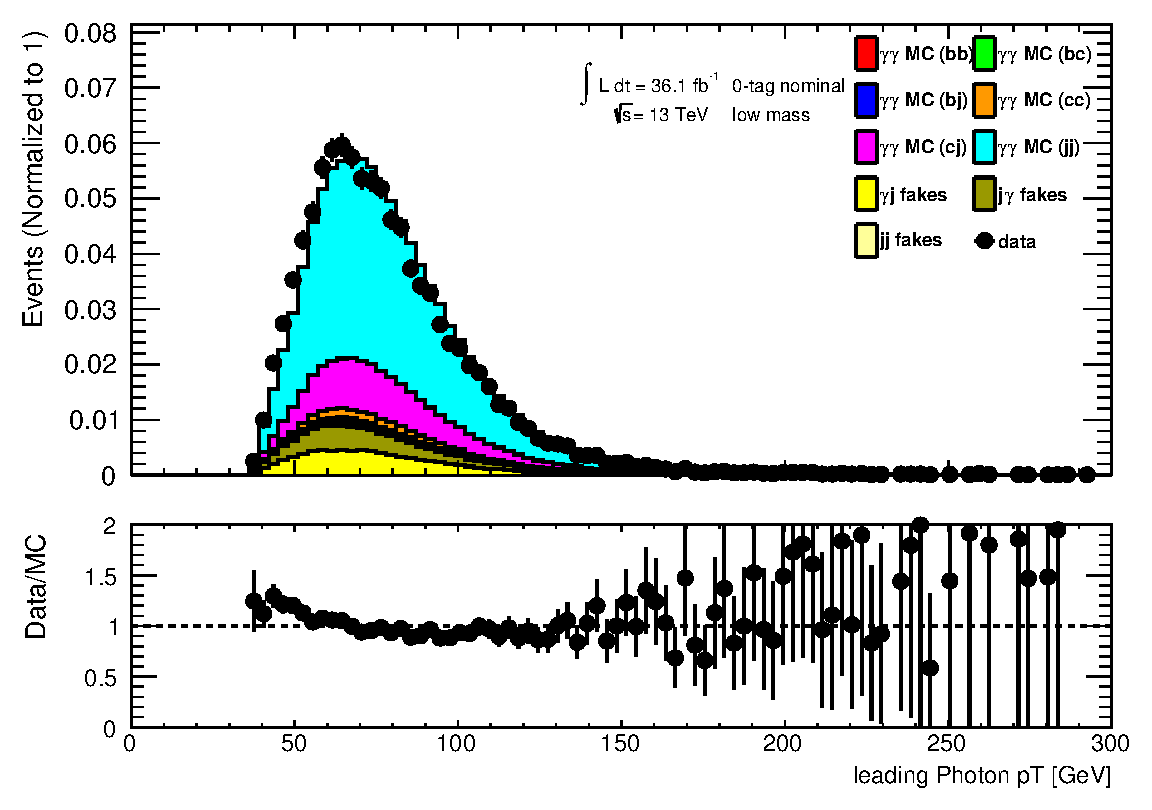
\includegraphics[width=0.48\textwidth]{chapters/chapter5_yybb/images/data_MC_comparison/h_CR_l_0t_nominal_leadingPhoton_pt.pdf}
  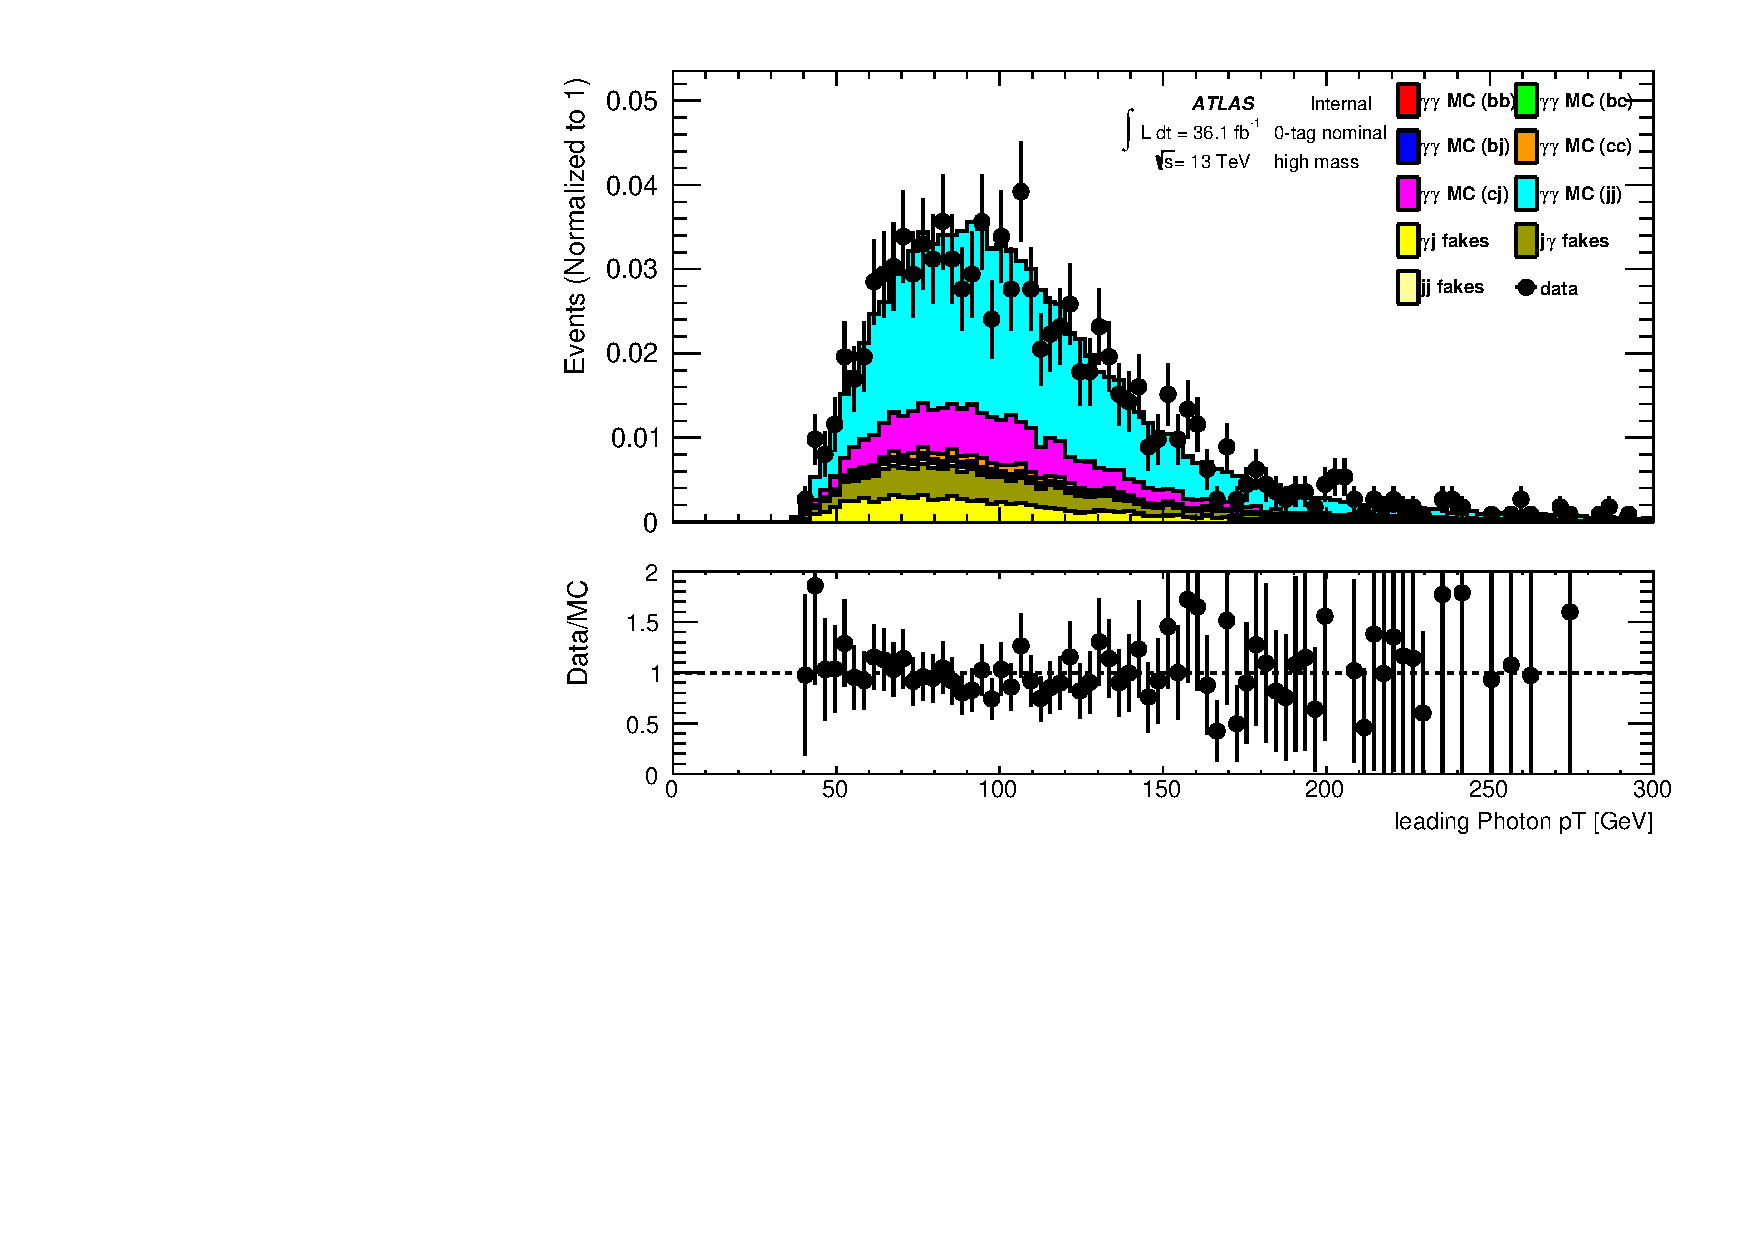
\includegraphics[width=0.48\textwidth]{chapters/chapter5_yybb/images/data_MC_comparison/h_CR_h_0t_nominal_leadingPhoton_pt.pdf}
  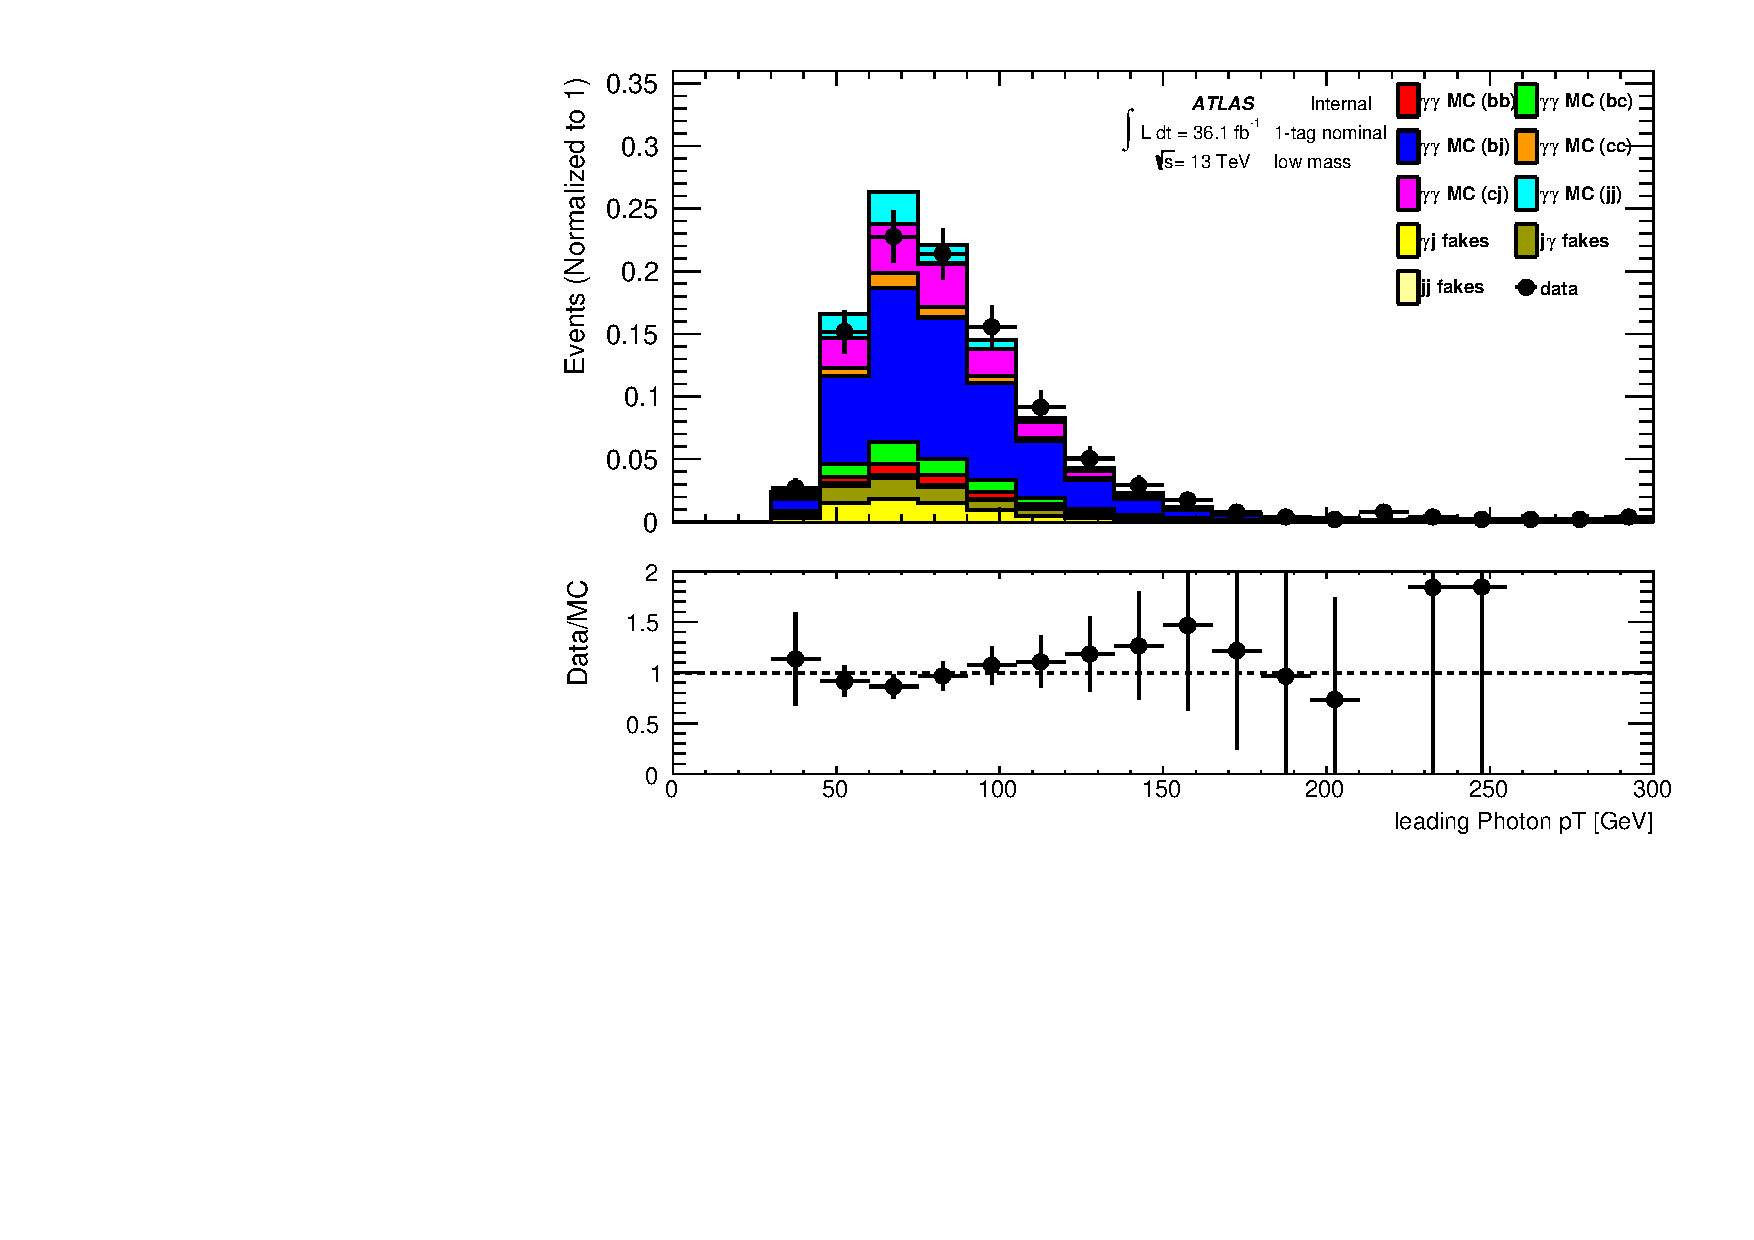
\includegraphics[width=0.48\textwidth]{chapters/chapter5_yybb/images/data_MC_comparison/h_SR_l_1t_nominal_leadingPhoton_pt.pdf}
  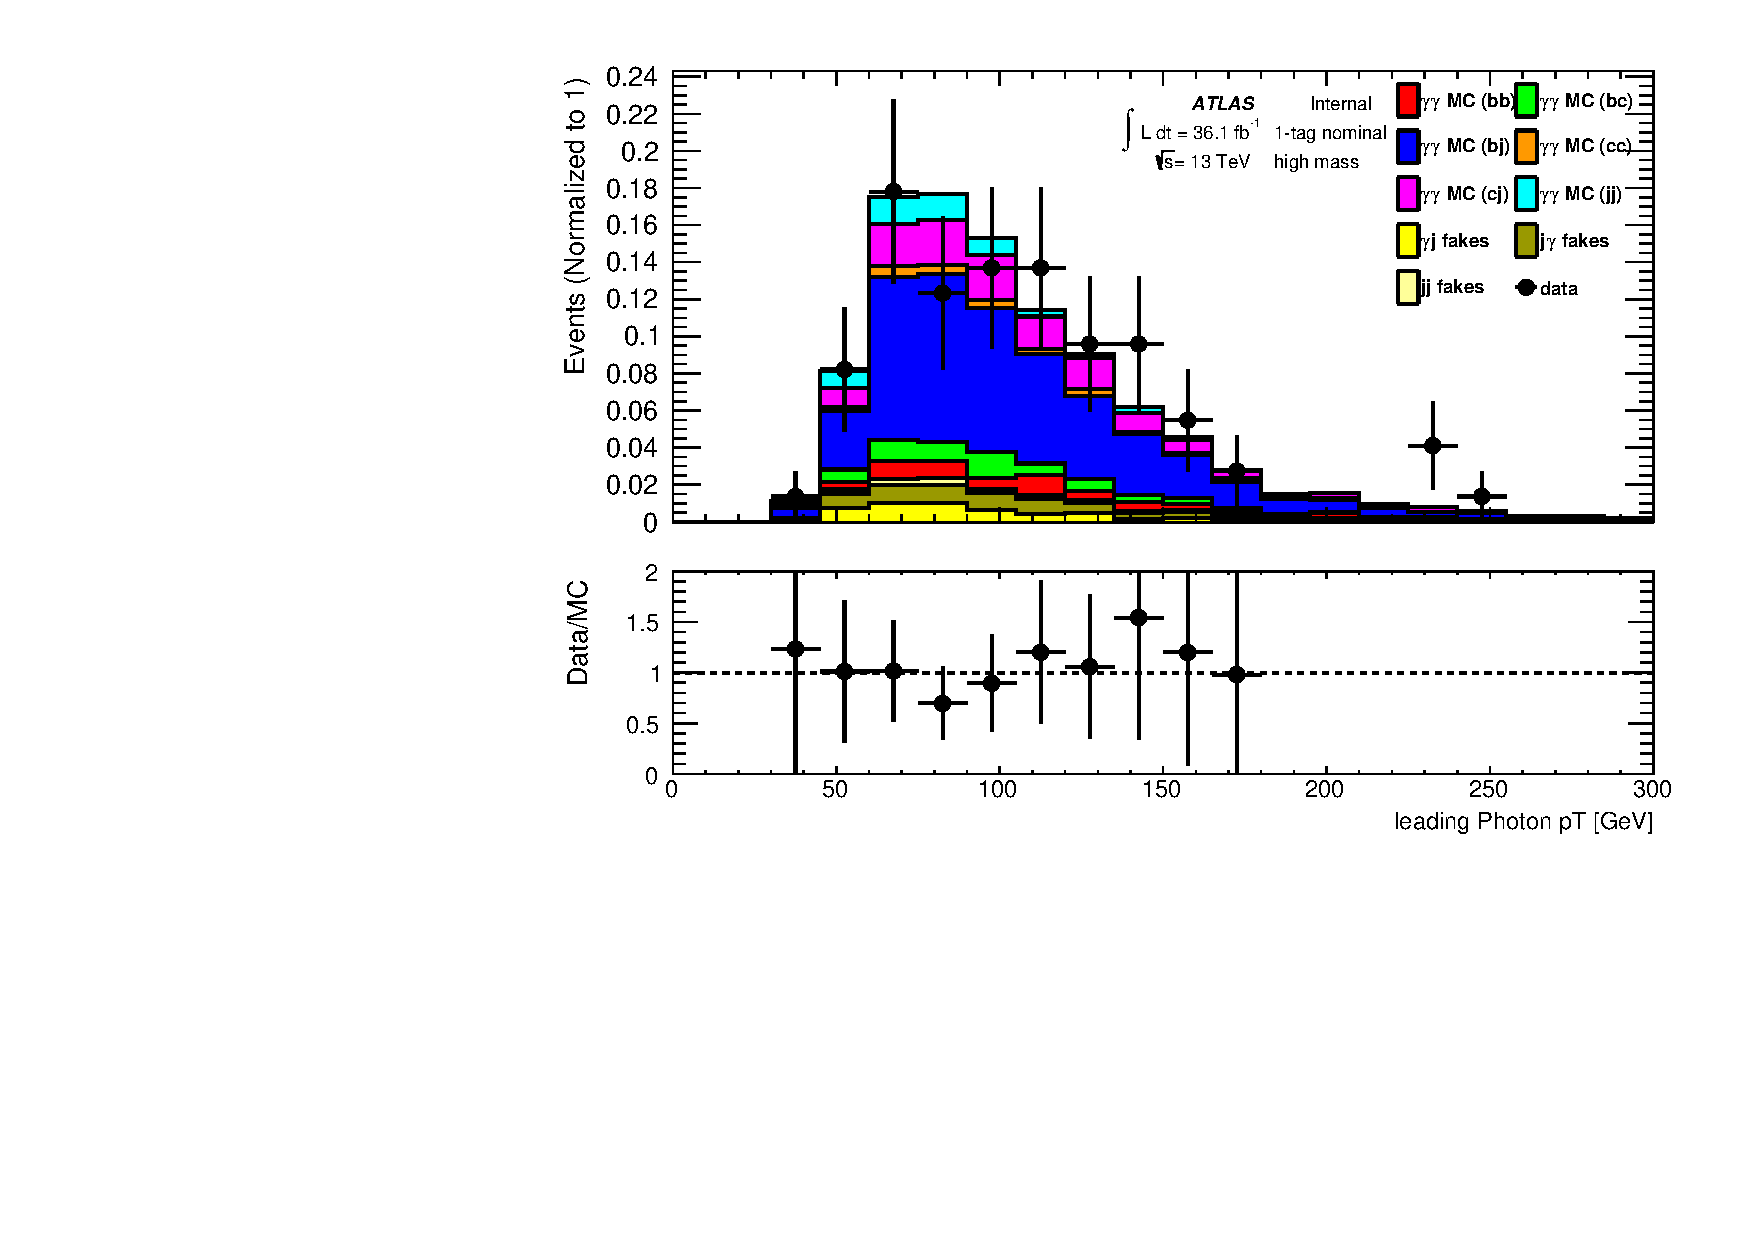
\includegraphics[width=0.48\textwidth]{chapters/chapter5_yybb/images/data_MC_comparison/h_SR_h_1t_nominal_leadingPhoton_pt.pdf}
  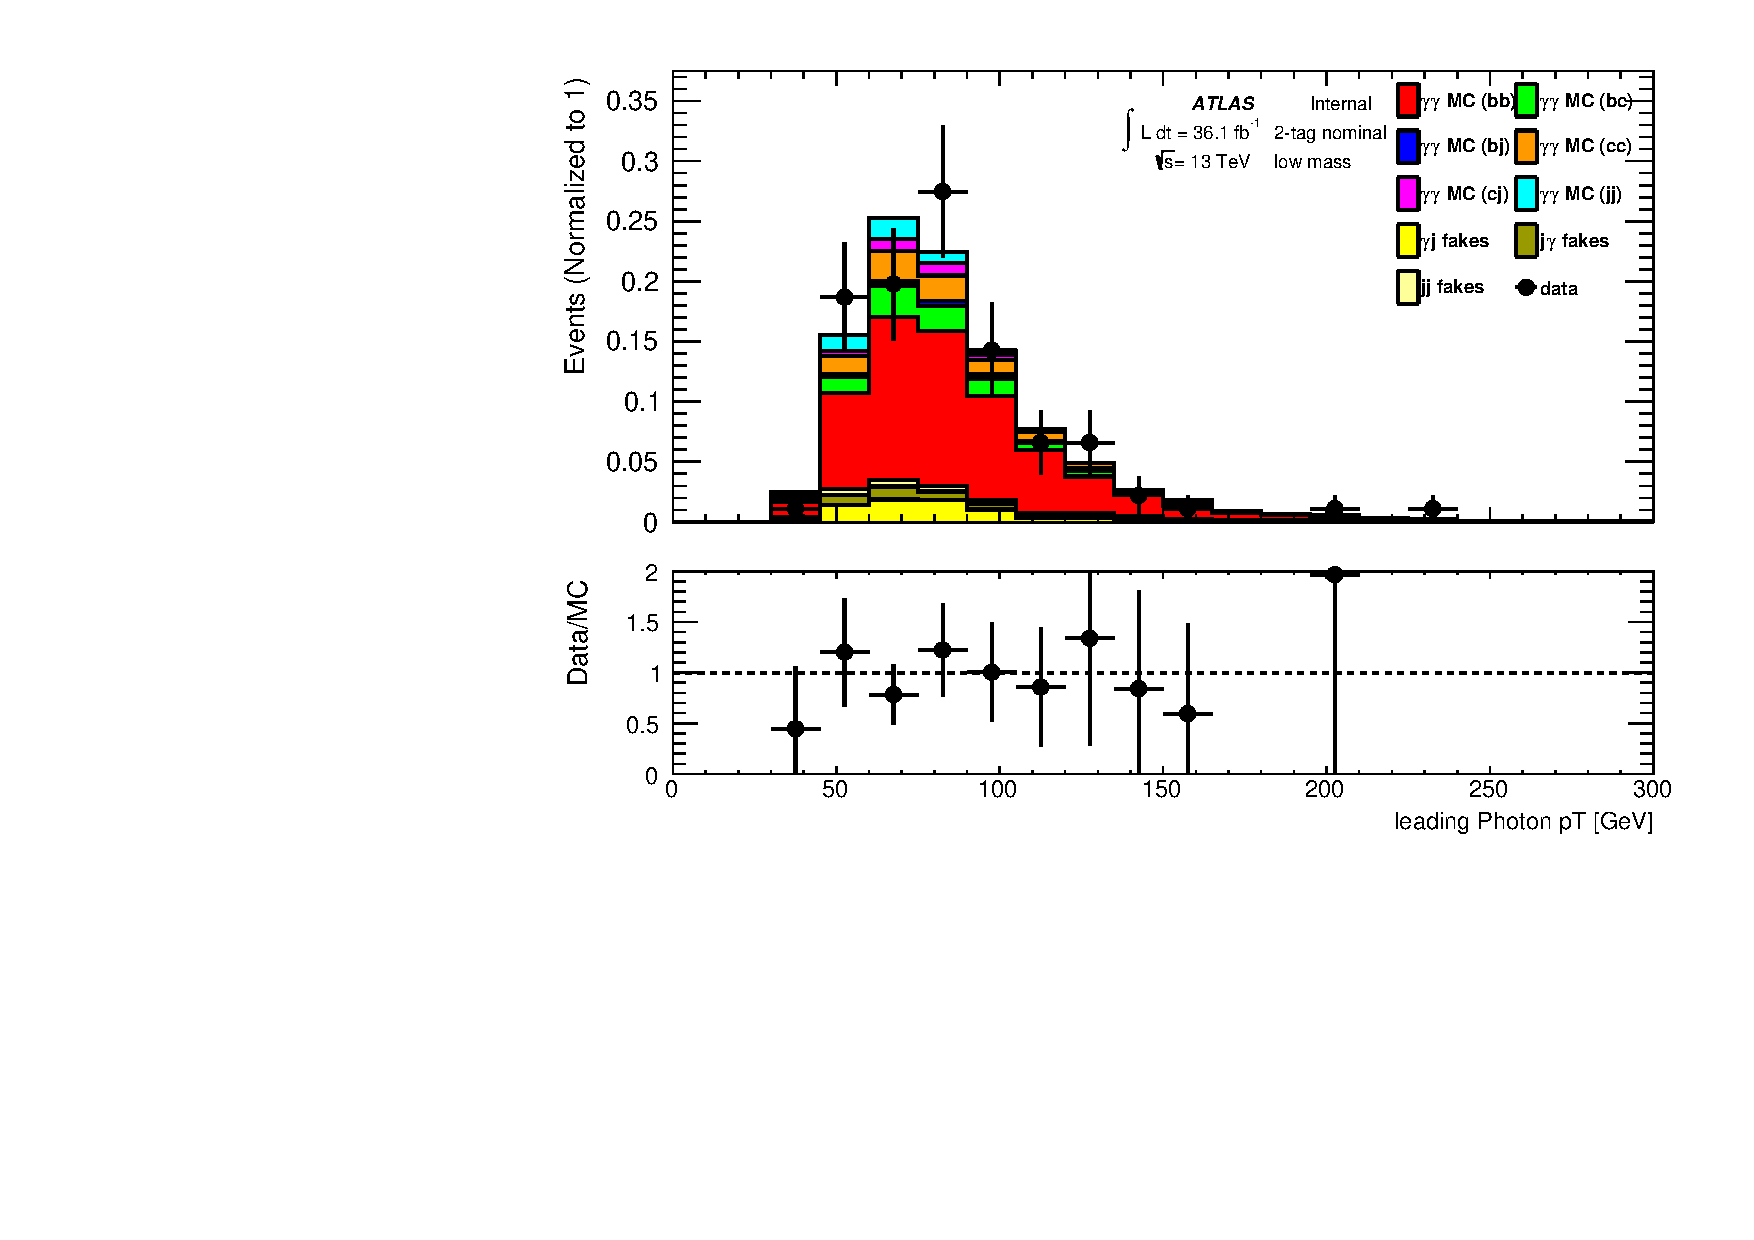
\includegraphics[width=0.48\textwidth]{chapters/chapter5_yybb/images/data_MC_comparison/h_SR_l_2t_nominal_leadingPhoton_pt.pdf}
  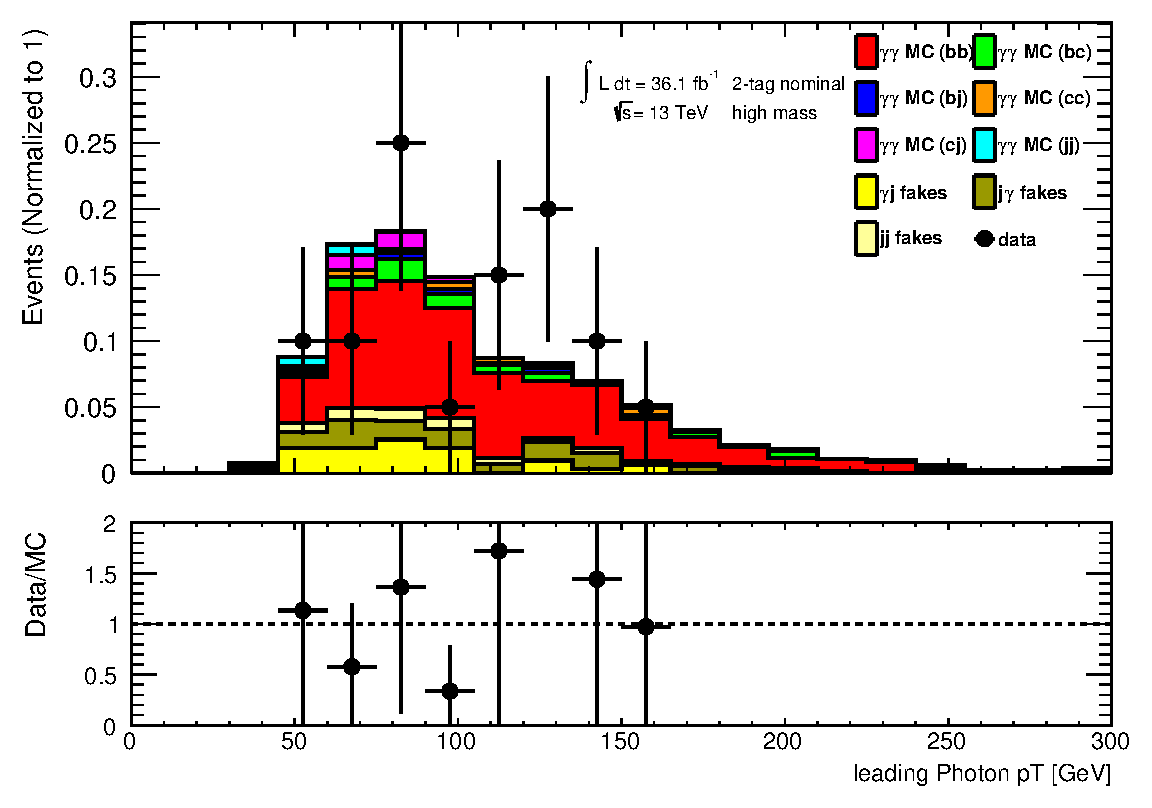
\includegraphics[width=0.48\textwidth]{chapters/chapter5_yybb/images/data_MC_comparison/h_SR_h_2t_nominal_leadingPhoton_pt.pdf}
  \caption[Leading photon \pt.]{Leading photon \pt by b-tagging category. The low (left) and high (right) mass selections are shown. Both data and MC are normalized such that the integral is 1.
  \label{fig:photon_l_pt}}
\end{figure}

\begin{figure}[p]
  \centering
  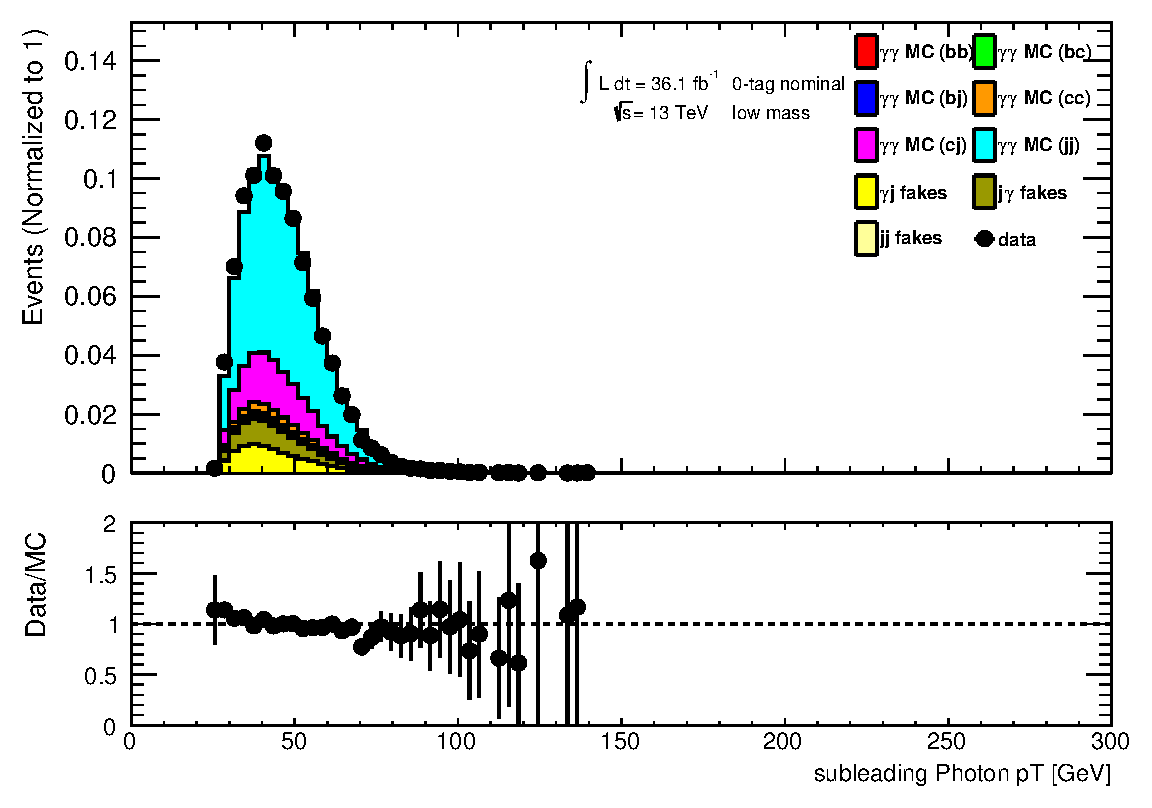
\includegraphics[width=0.48\textwidth]{chapters/chapter5_yybb/images/data_MC_comparison/h_CR_l_0t_nominal_subleadingPhoton_pt.pdf}
  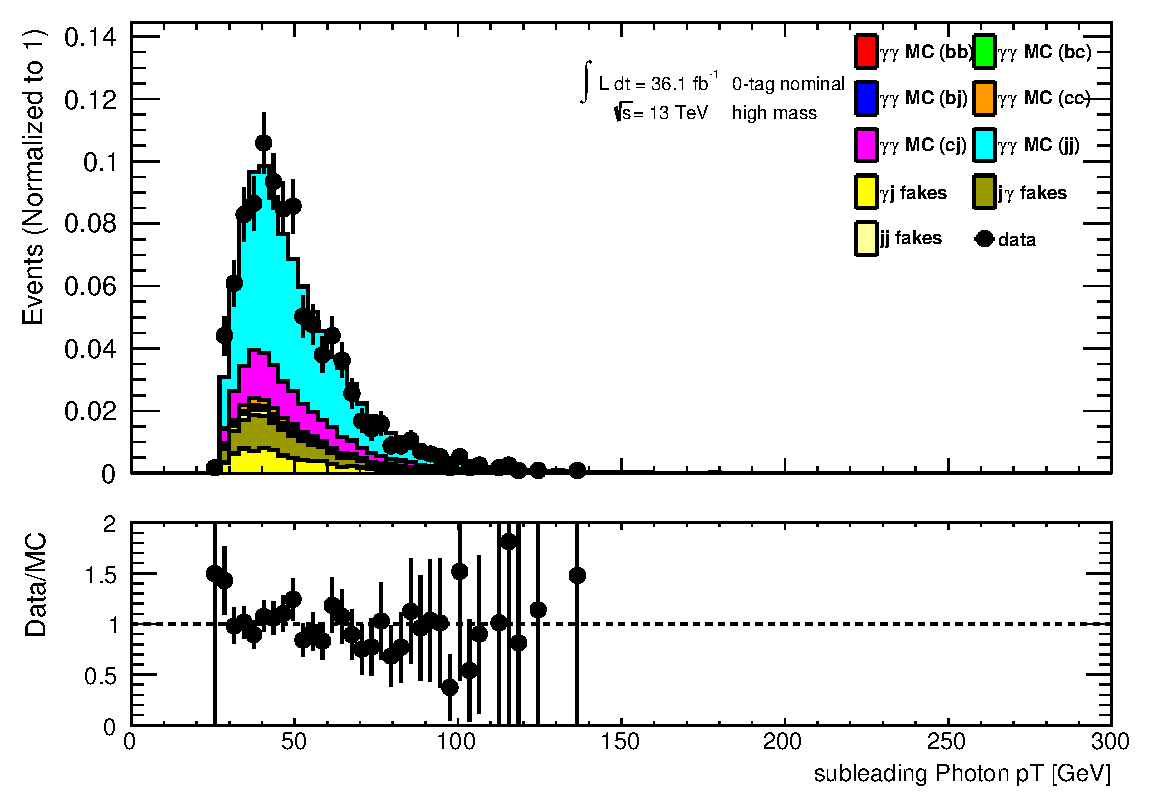
\includegraphics[width=0.48\textwidth]{chapters/chapter5_yybb/images/data_MC_comparison/h_CR_h_0t_nominal_subleadingPhoton_pt.pdf}
  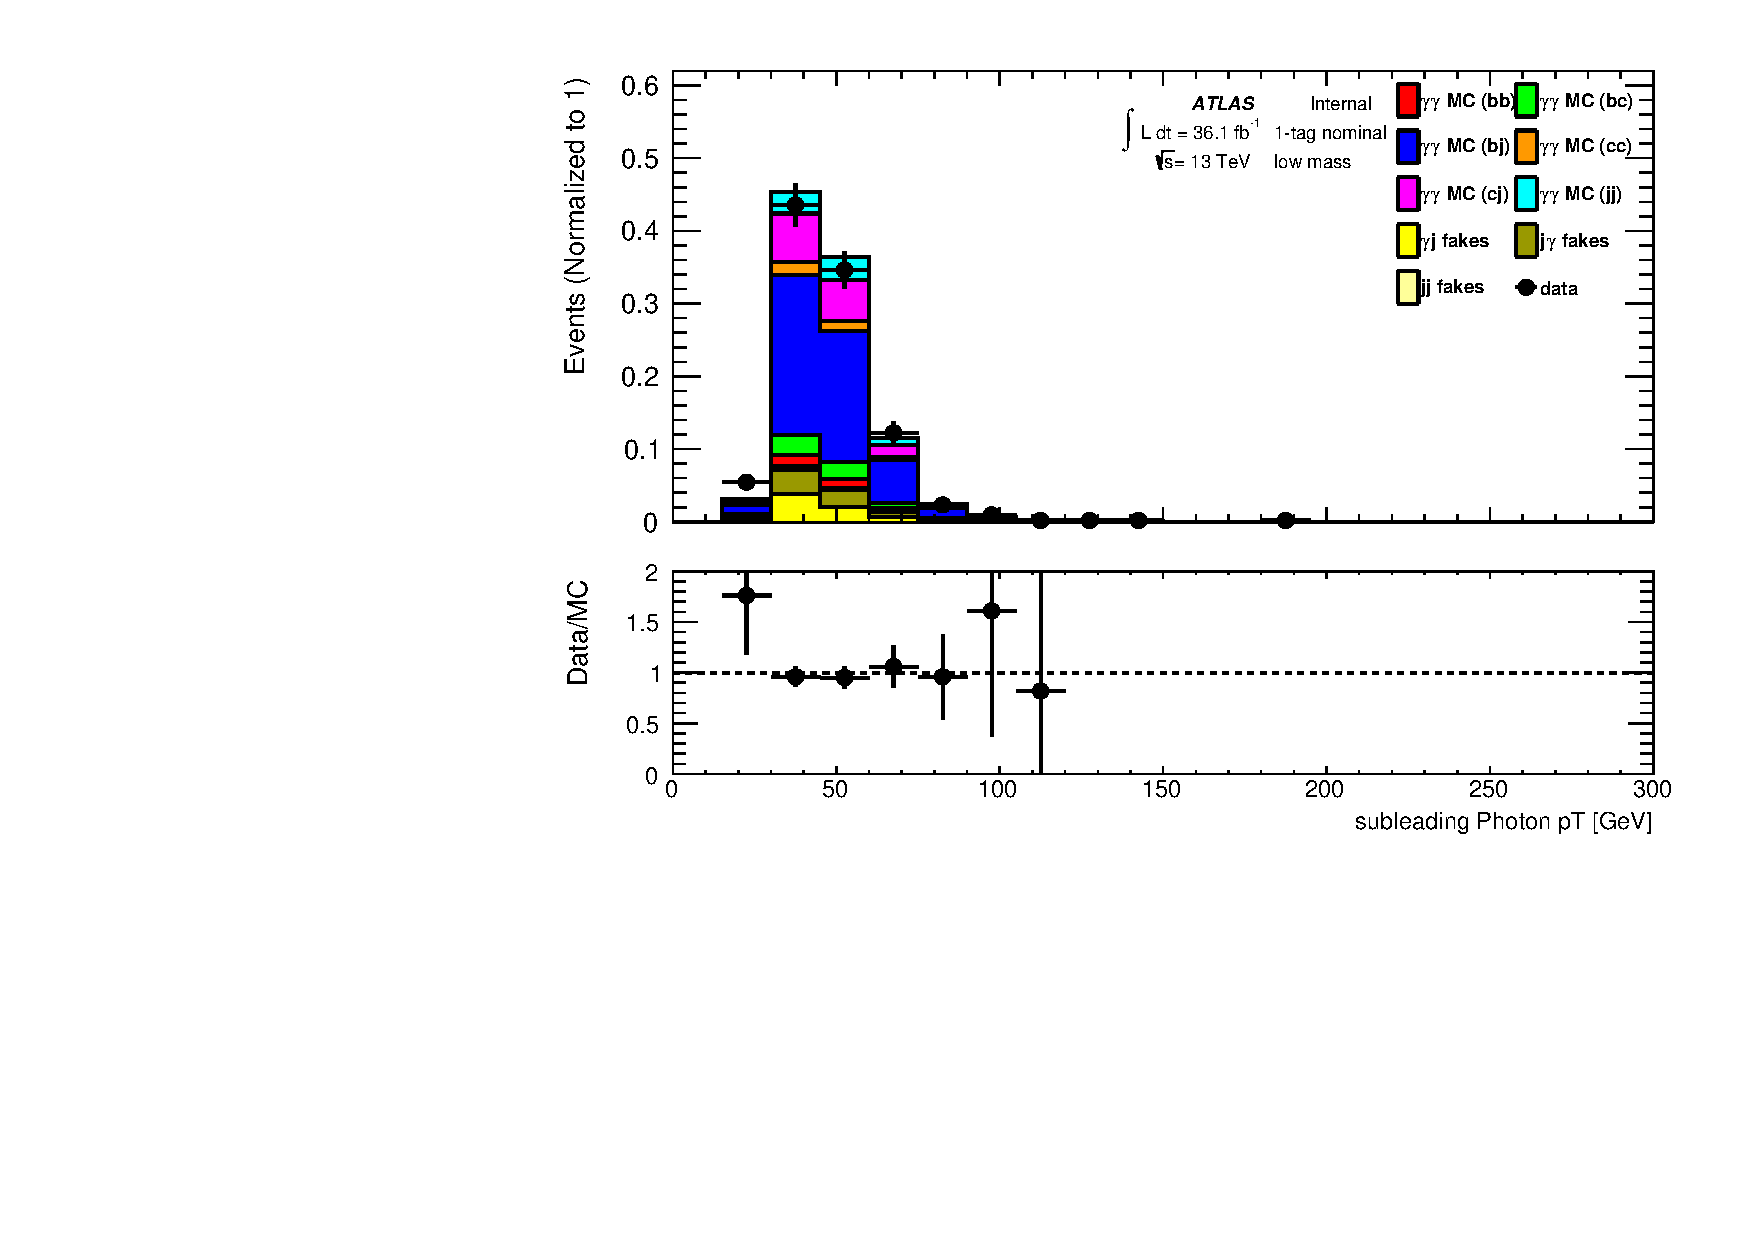
\includegraphics[width=0.48\textwidth]{chapters/chapter5_yybb/images/data_MC_comparison/h_SR_l_1t_nominal_subleadingPhoton_pt.pdf}
  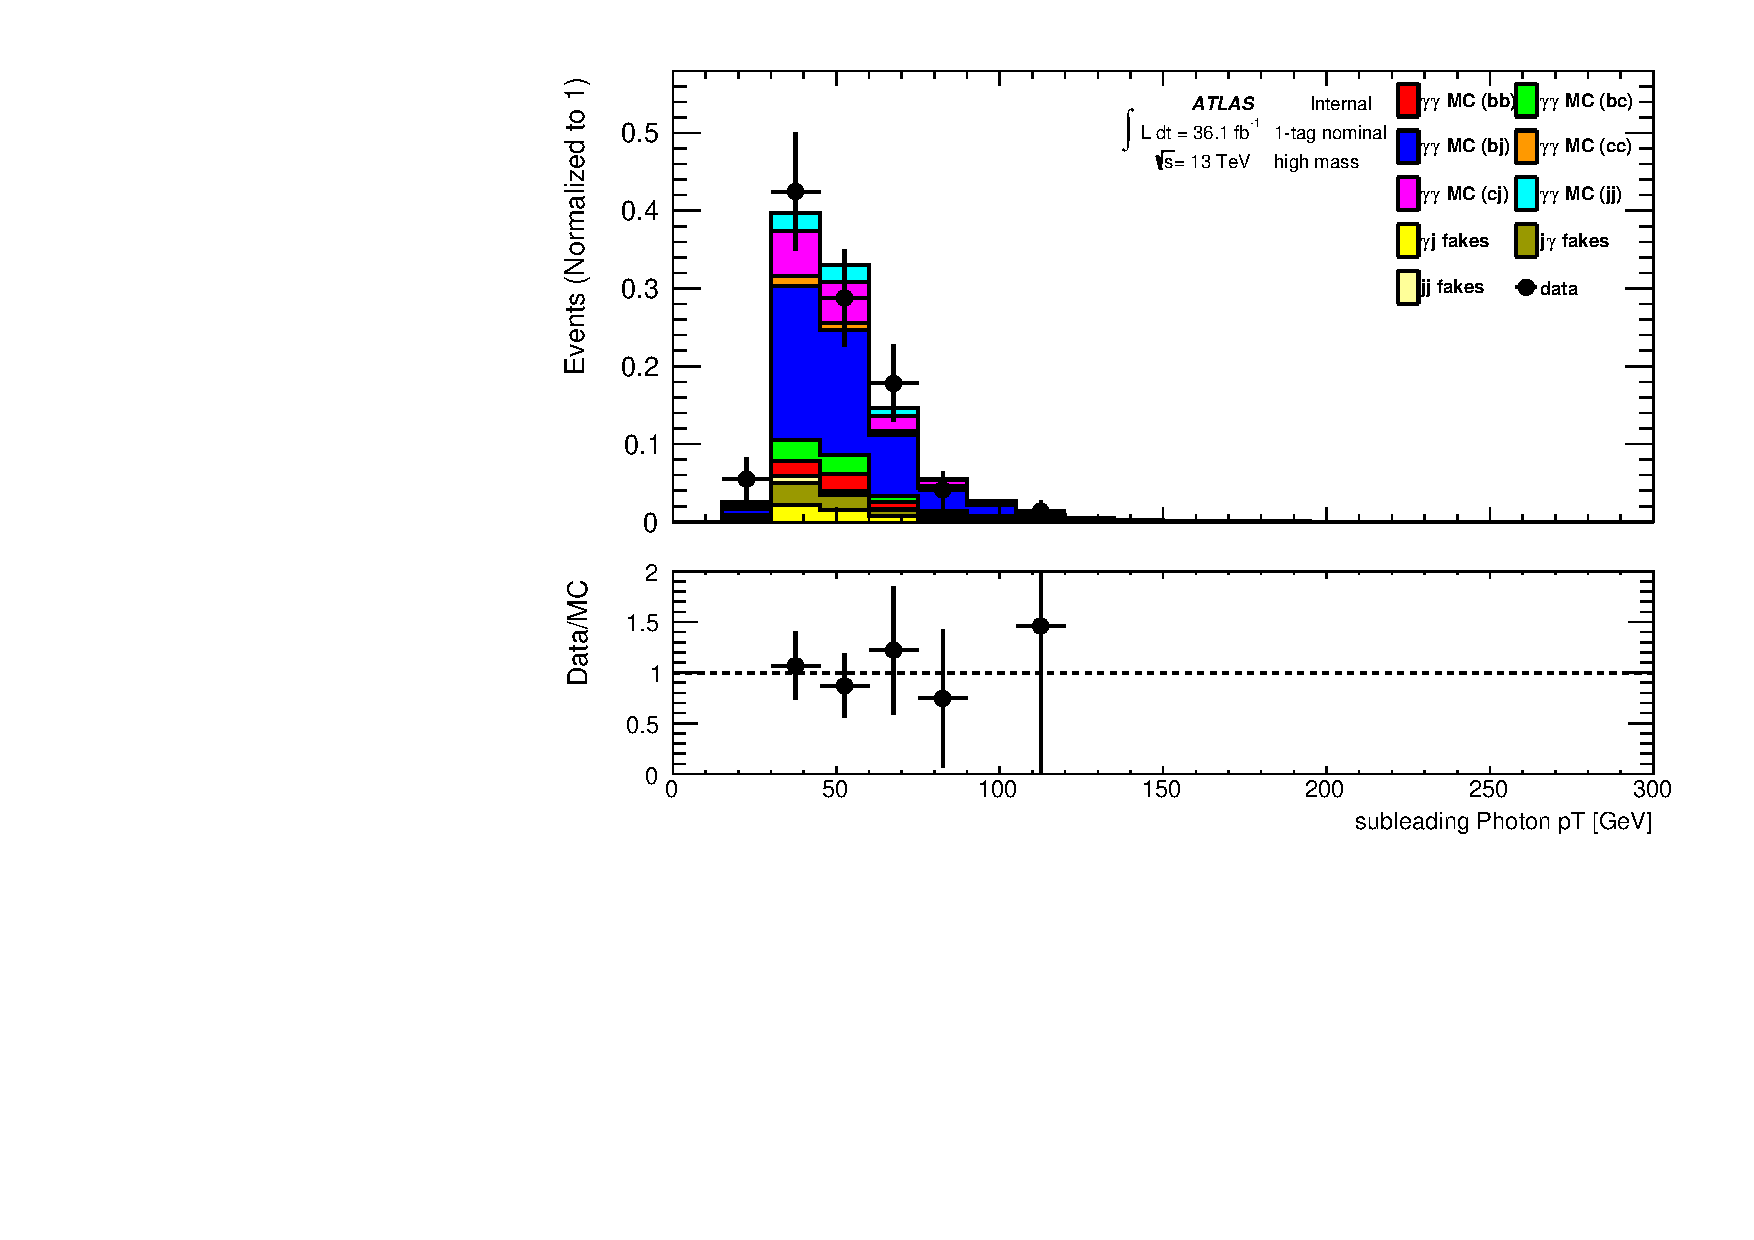
\includegraphics[width=0.48\textwidth]{chapters/chapter5_yybb/images/data_MC_comparison/h_SR_h_1t_nominal_subleadingPhoton_pt.pdf}
  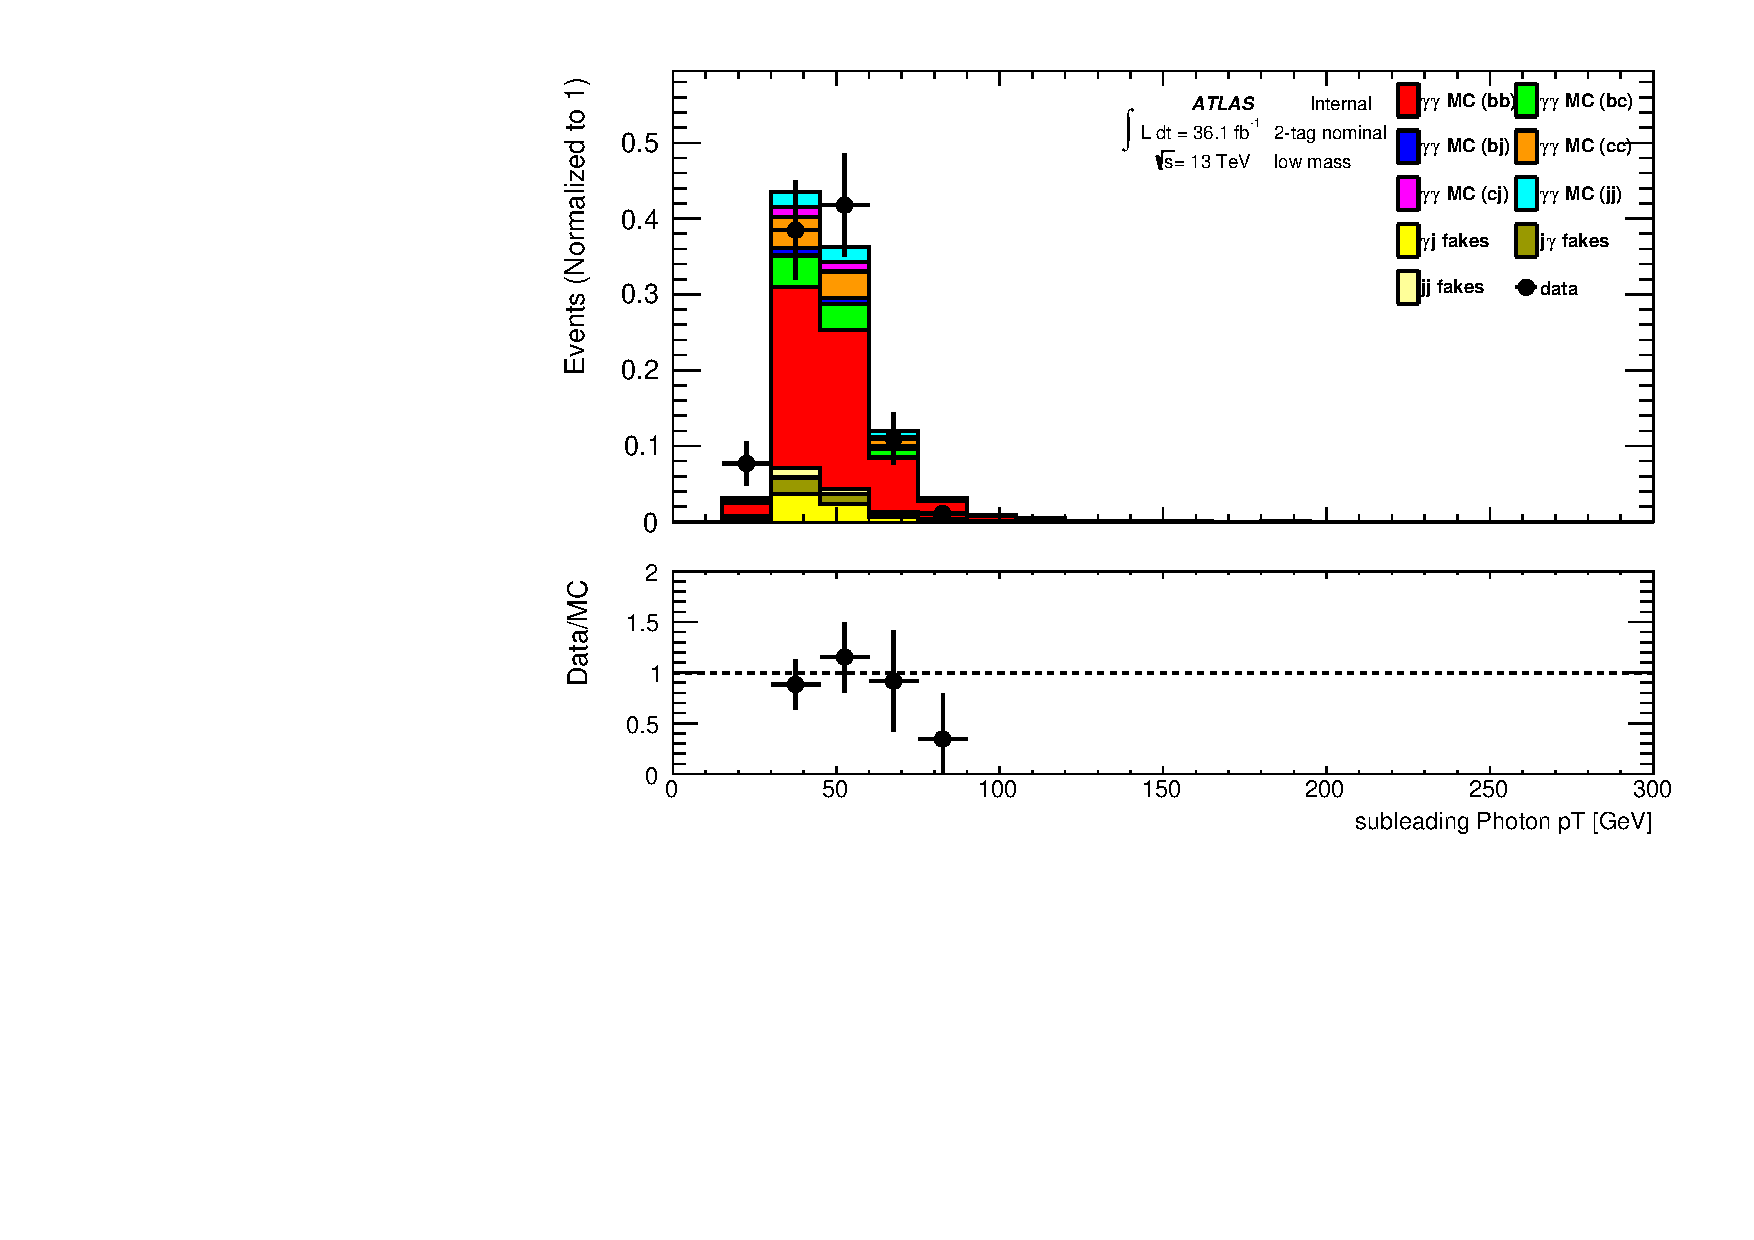
\includegraphics[width=0.48\textwidth]{chapters/chapter5_yybb/images/data_MC_comparison/h_SR_l_2t_nominal_subleadingPhoton_pt.pdf}
  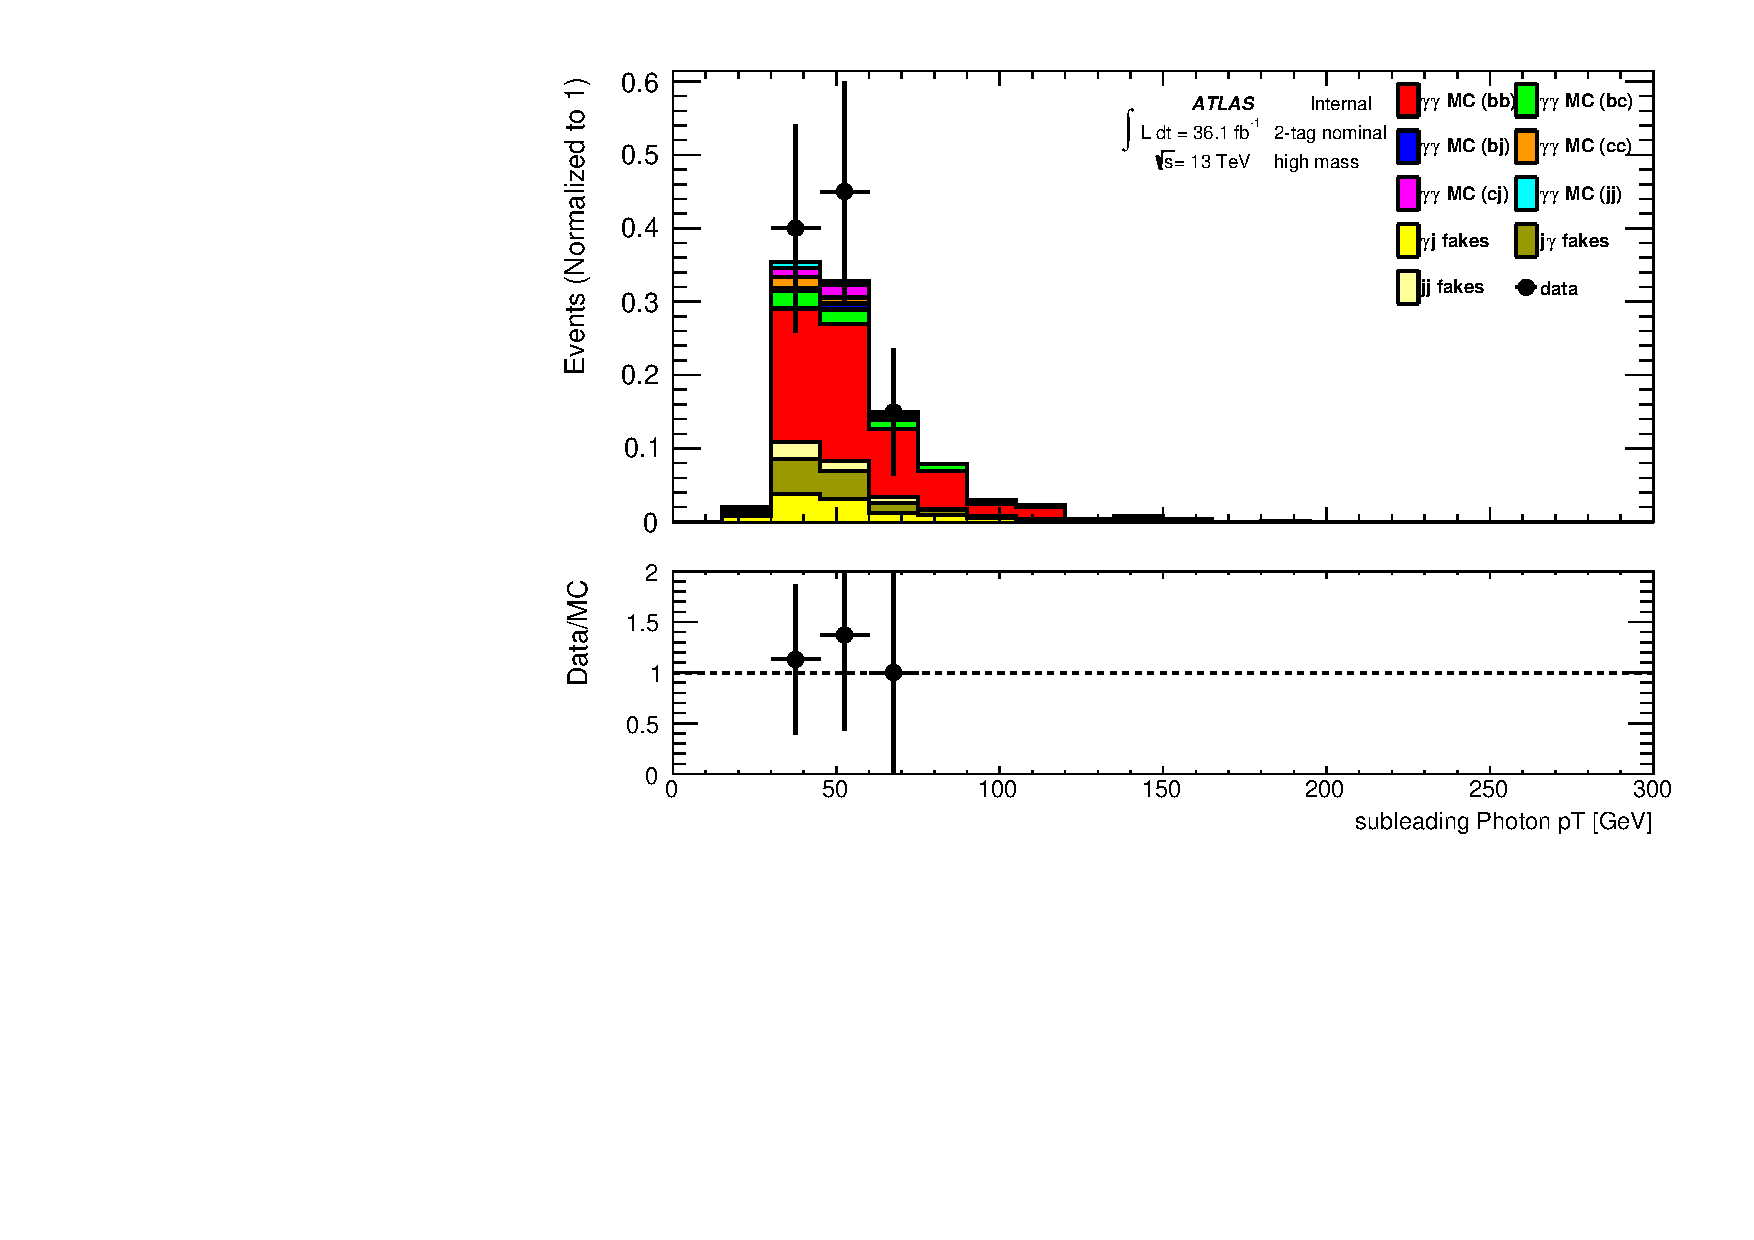
\includegraphics[width=0.48\textwidth]{chapters/chapter5_yybb/images/data_MC_comparison/h_SR_h_2t_nominal_subleadingPhoton_pt.pdf}
  \caption[Subleading photon \pt.]{Subleading photon \pt by b-tagging category. The low (left) and high (right) mass selections are shown. Both data and MC are normalized such that the integral is 1.
  \label{fig:photon_s_pt}}
\end{figure}

To select the \gls{PV}, a \gls{NN} is used. This \gls{NN} uses the following inputs:
\begin{itemize}
  \item $(z_{\text{common}} - z_{\text{vertex}})/(\sigma_z)$. $z_{\text{vertex}}$ is the position of the primary vertex. $z_{\text{common}}$ is defined by the weighted mean of extrapolated photon trajectories. For converted photons, this is replaced by the direction derived by connecting the conversion location to the cluster barycenter in the first sampling layer in the \gls{EM} calorimeter. $\sigma_z$ is the associated error.
  \item $\log(\sum \pt)$ of tracks
  \item $\log(\sum \pt^2)$ of tracks
  \item $\Delta \phi(\gamma\gamma,\text{PV})$. $\phi$ of the \gls{PV} is defined as the $\phi$ vector sum of tracks associated to the vertex
  
\end{itemize}
After selecting this \gls{PV}, tracking and calorimeter variables are recomputed with respect to the new chosen \gls{PV}. This method is greater than 85\% efficient at selecting the correct \gls{PV}.


\subsection{Jets}

Jets are reconstructed with the \path{FastJet} \cite{fastjet} package. They are defined using the \antikt algorithm with $R=0.4$, using jets with energy corrected for pile-up effects and direction readjusted to the primary vertex (EM-JES jets). Jets considered must have $\pt > \unit{25}{\GeV}$ and be within the tagging region, $\abseta < 2.5$. The following additional requirements are applied\footnote{This selection is similar to that of the default jet selection for ATLAS $H\rightarrow \yy$ analyses. The $\abseta < 2.5$ is an additional requirement imposed atop that selection for b-tagging.}:

\begin{itemize}
  \item Jets with $\pt < \unit{50}{\GeV}$ and $\abseta < 2.4$ must pass the ``default'' \gls{JVT} requirement, with $|\text{JVT}| \geq 0.59$ \cite{JVT}.
  \item Events that contain a jet passing the ``LooseBad'' cut are vetoed. 
  \item Jets with $\Dr < 0.4$ from a tight, isolated photon are vetoed.
  \item Jets with $\Dr < 0.2$ from a selected electron are vetoed.
\end{itemize}



Following this selection, candidate jets are selected in the following way:
\begin{itemize}
  \item In the 0-tag control region, the two leading jets are the candidate jets.
  \item In the 1-tag region, one of the jets is the b-tagged jet, the other is selected via a \gls{BDT}
  \item In the 2-tag region, the two b-tagged jets are the candidate jets.
\end{itemize}

\begin{figure}[p] %TODO cite me
  \centering
  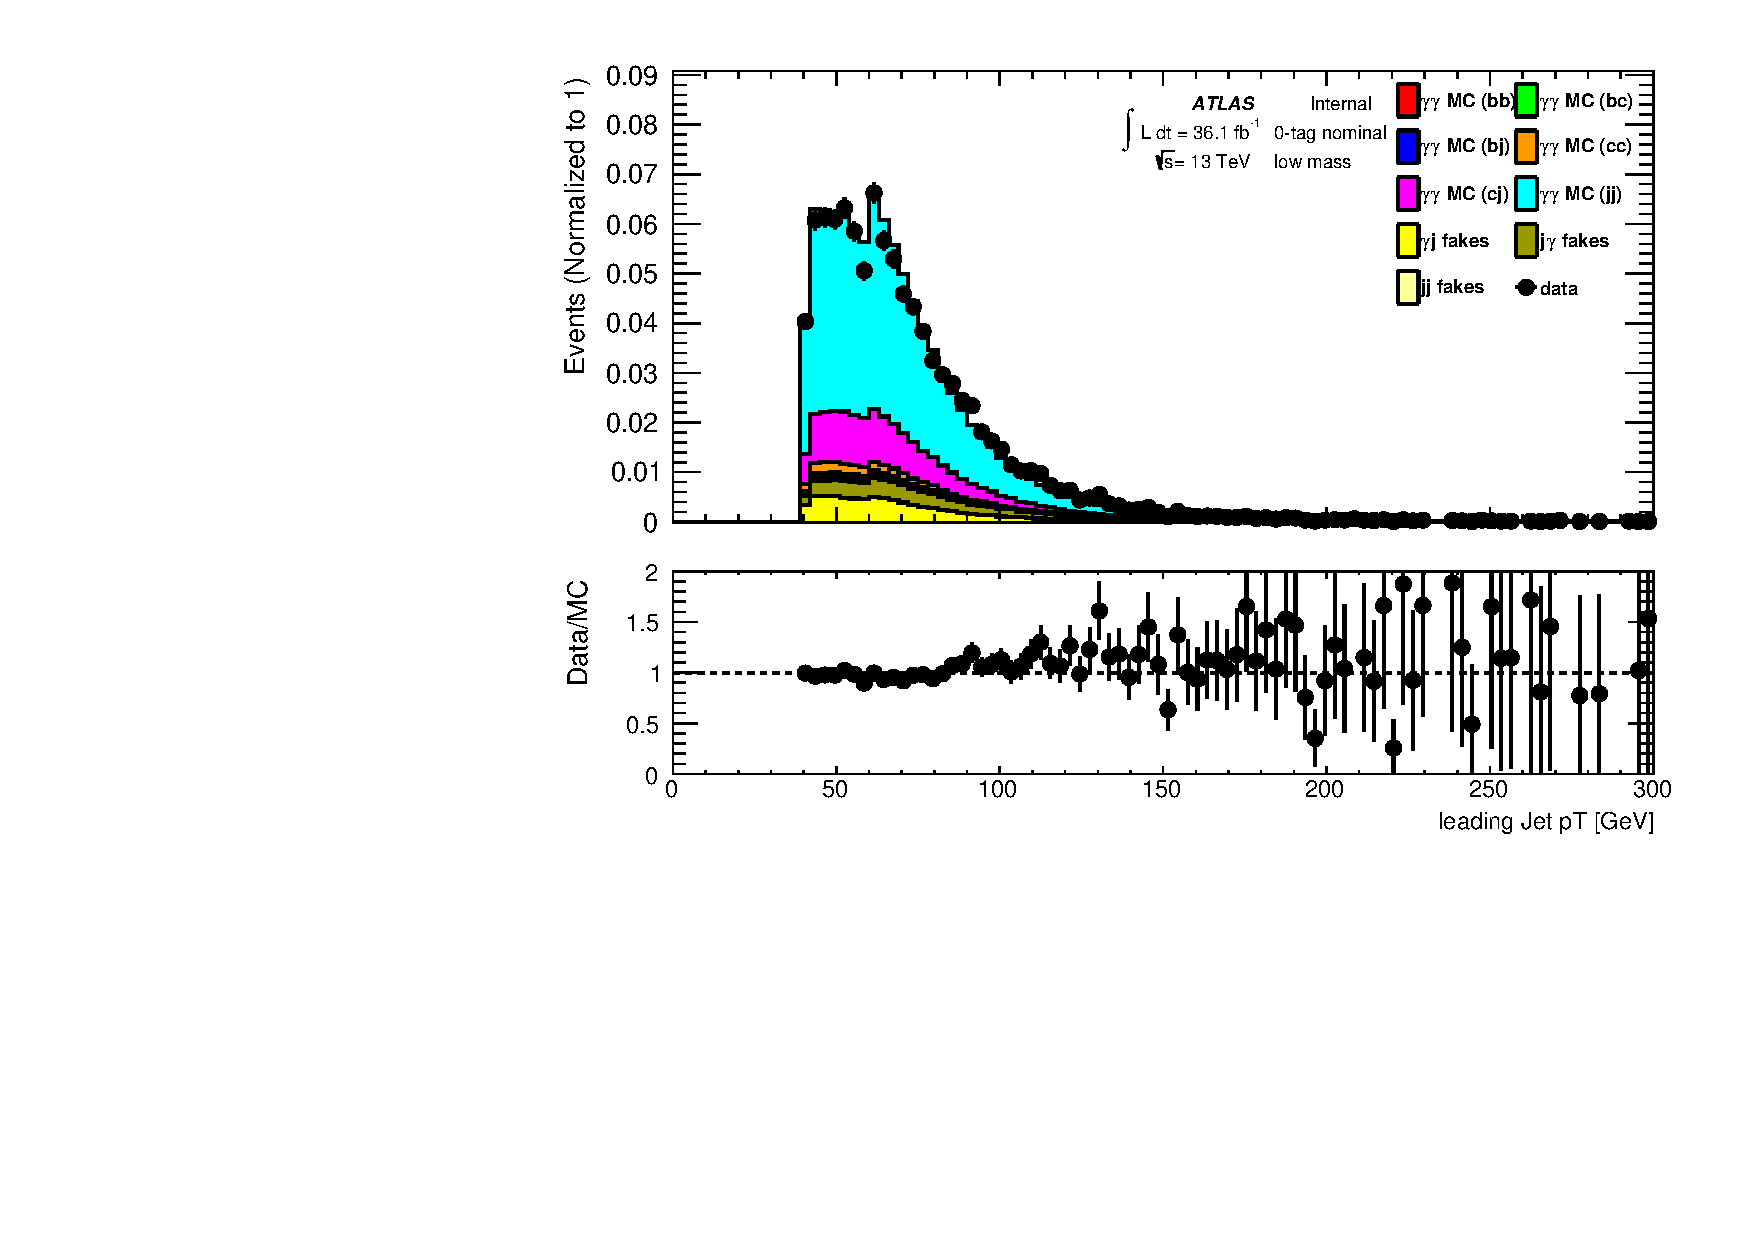
\includegraphics[width=0.48\textwidth]{chapters/chapter5_yybb/images/data_MC_comparison/h_CR_l_0t_nominal_leadingJet_pt.pdf}
  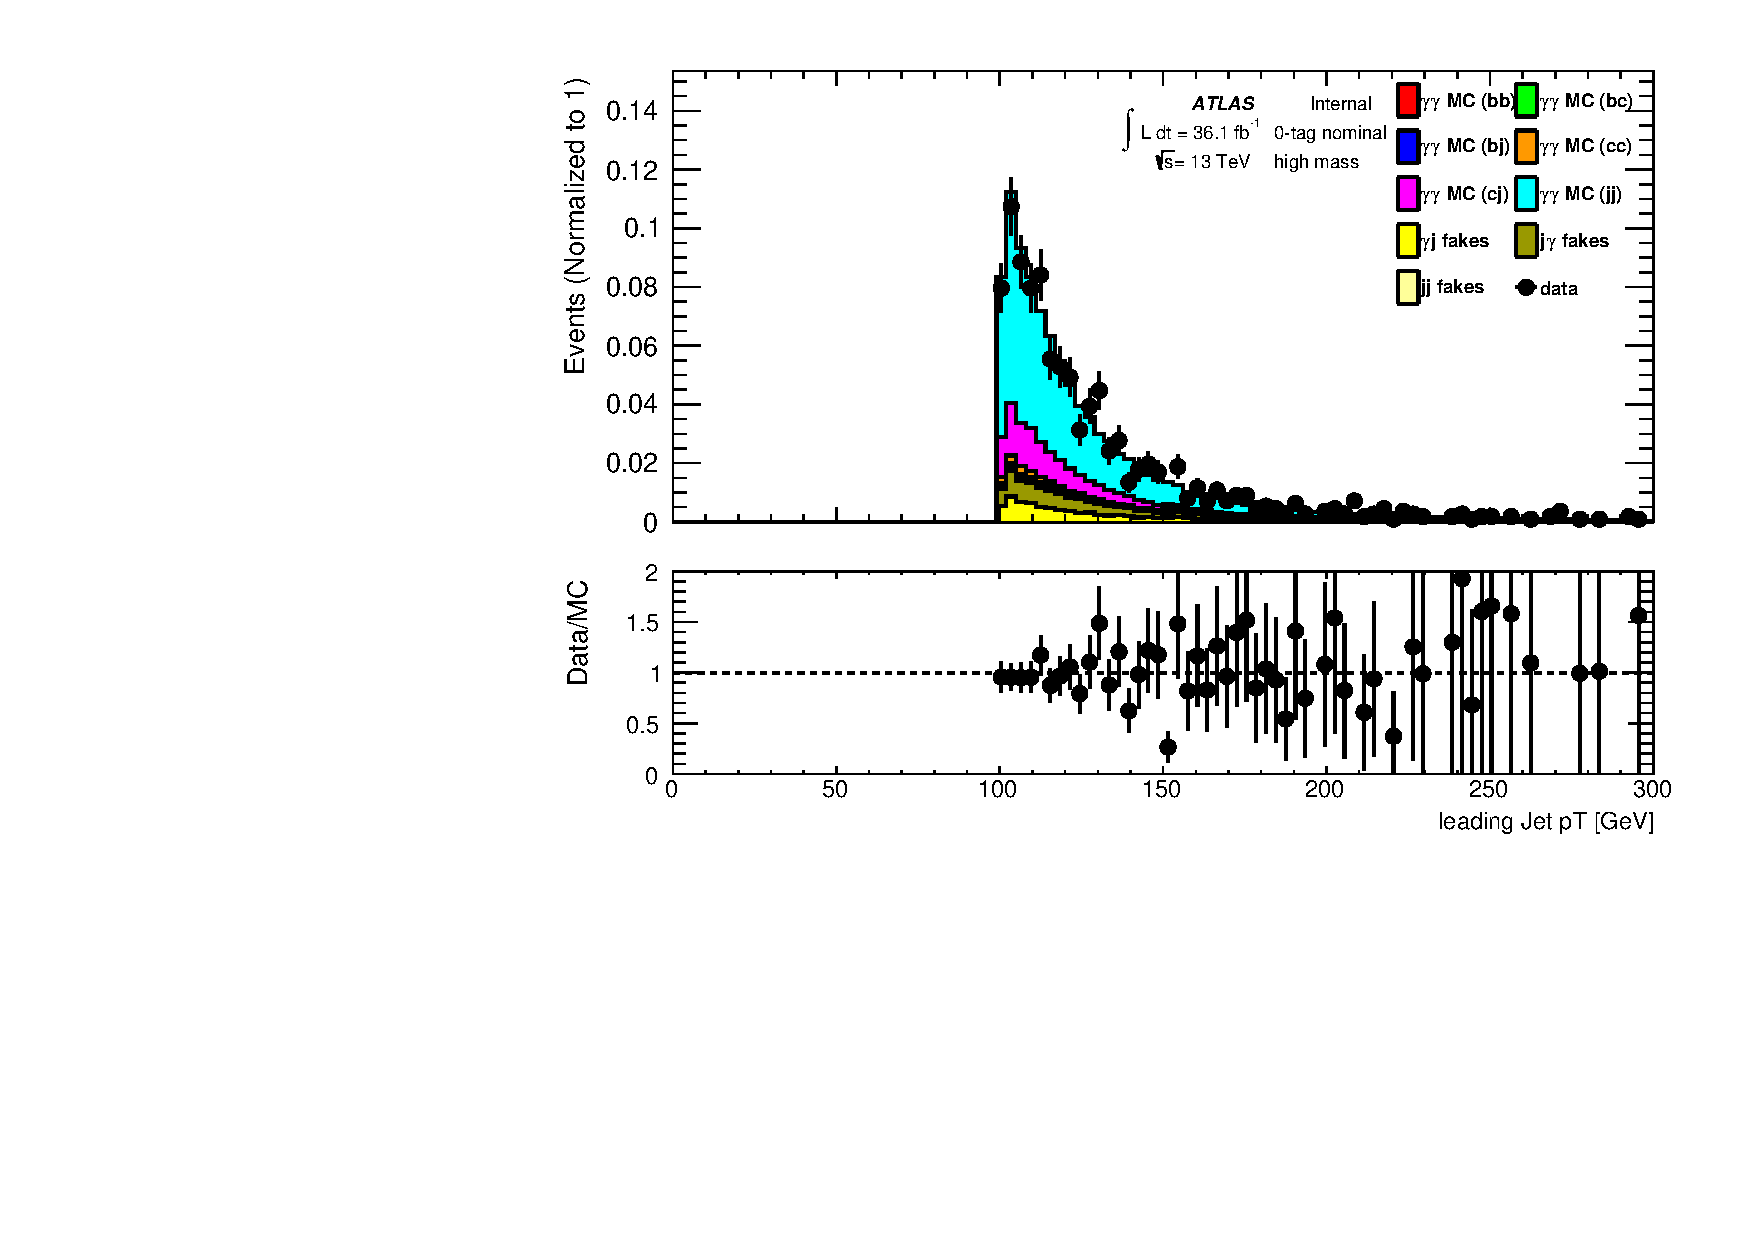
\includegraphics[width=0.48\textwidth]{chapters/chapter5_yybb/images/data_MC_comparison/h_CR_h_0t_nominal_leadingJet_pt.pdf}
  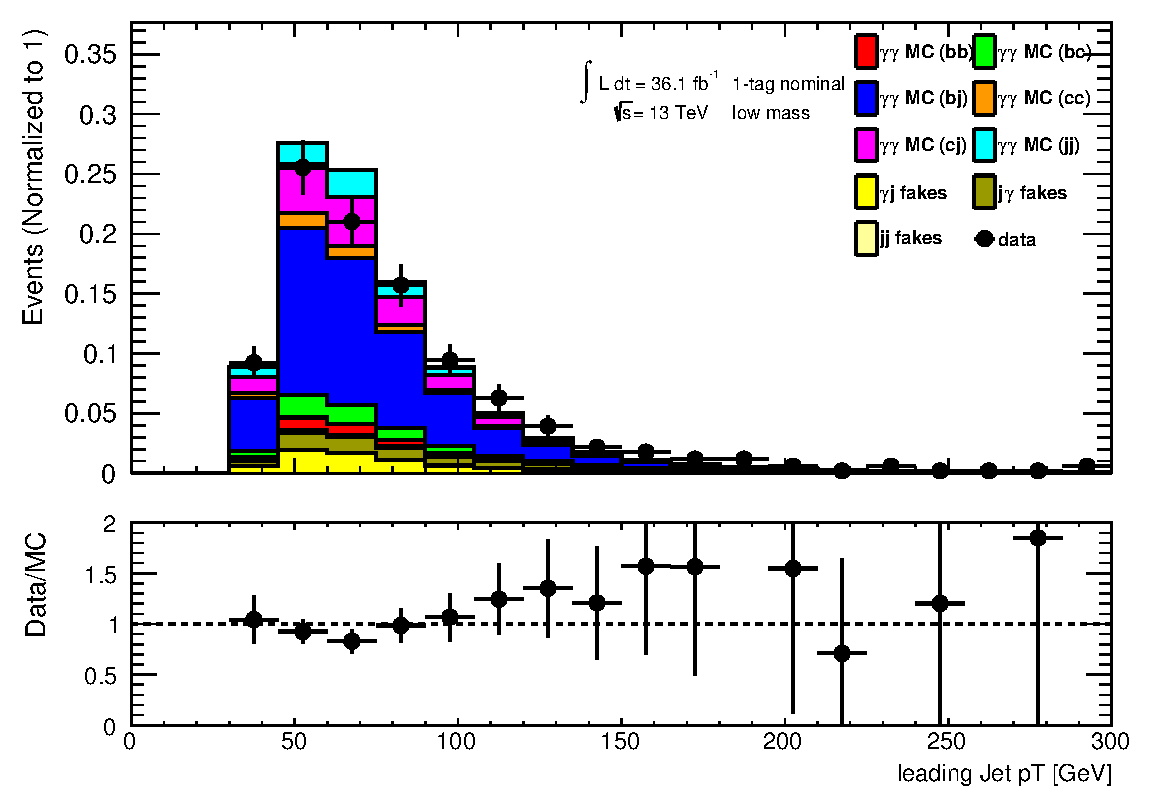
\includegraphics[width=0.48\textwidth]{chapters/chapter5_yybb/images/data_MC_comparison/h_SR_l_1t_nominal_leadingJet_pt.pdf}
  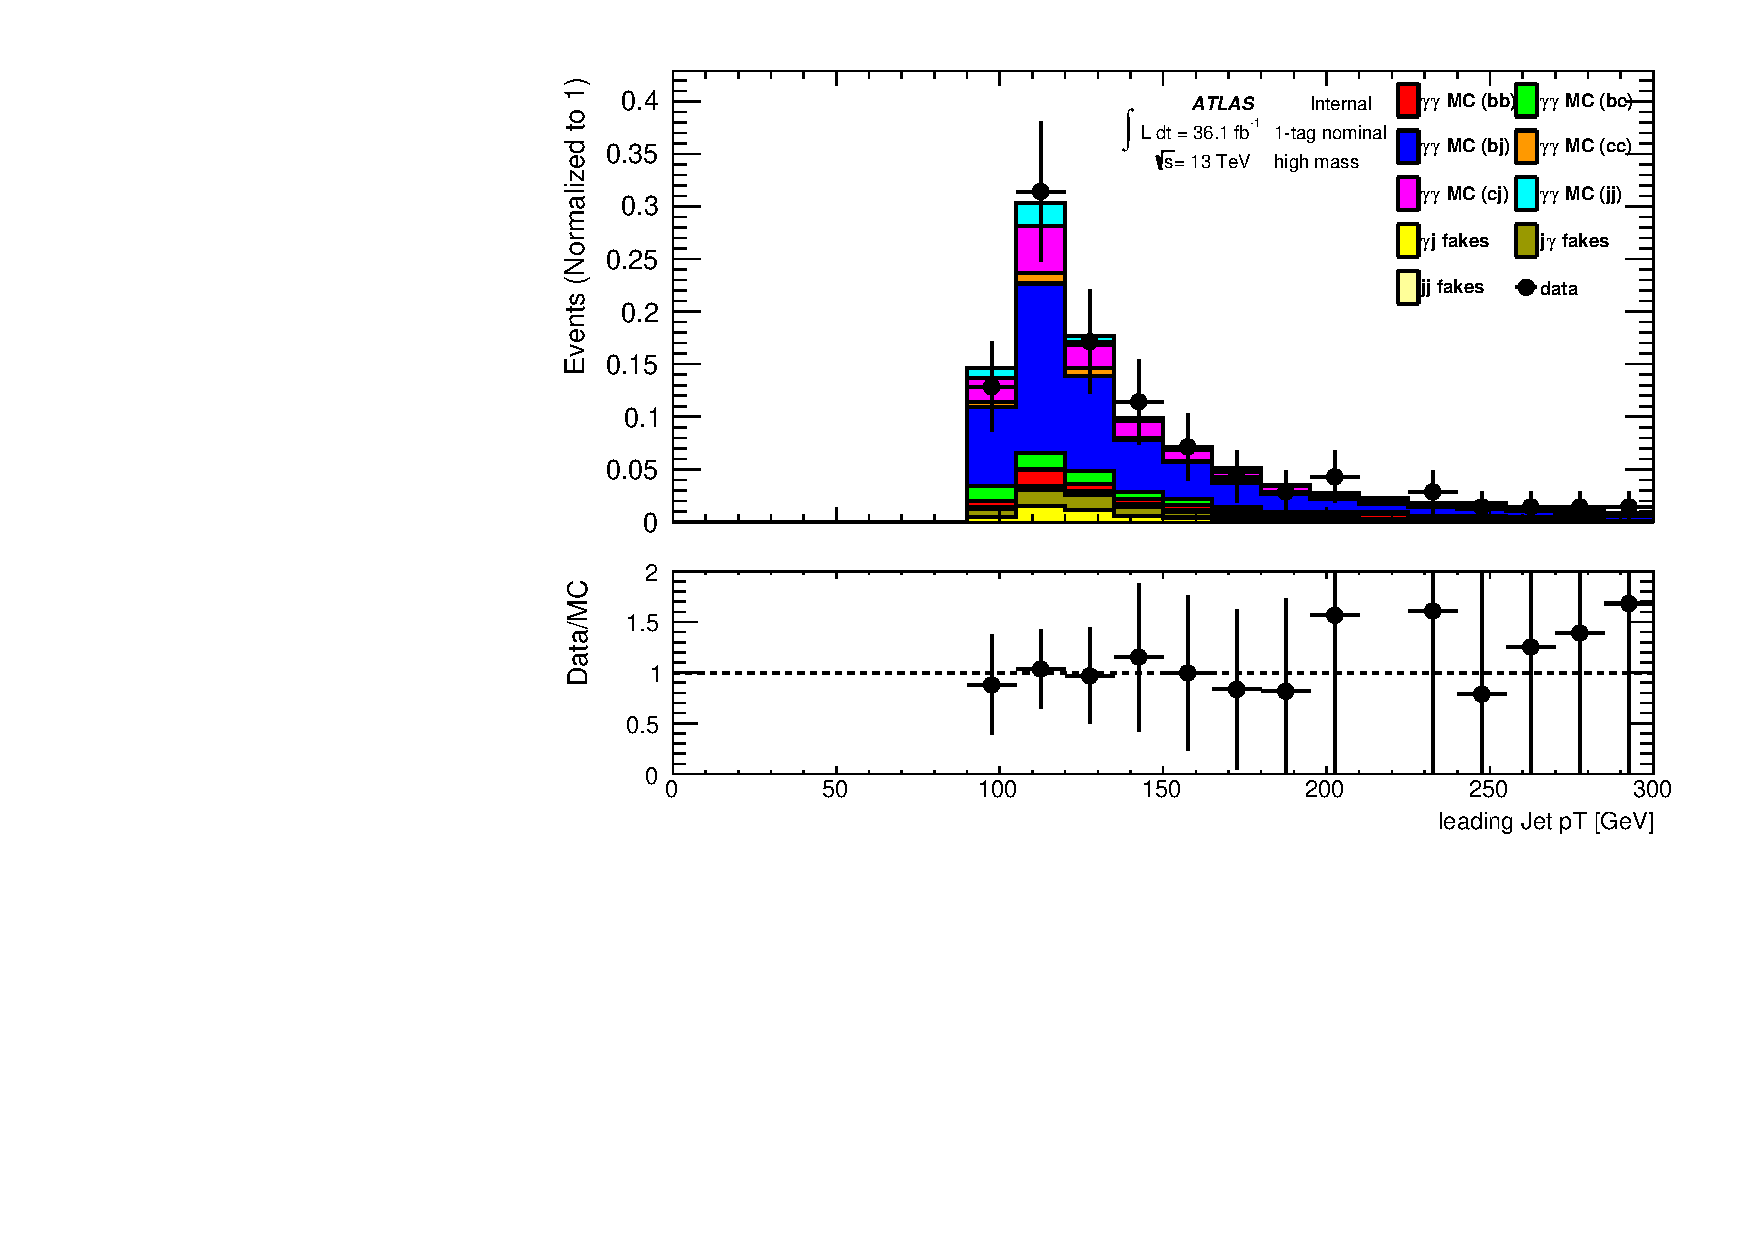
\includegraphics[width=0.48\textwidth]{chapters/chapter5_yybb/images/data_MC_comparison/h_SR_h_1t_nominal_leadingJet_pt.pdf}
  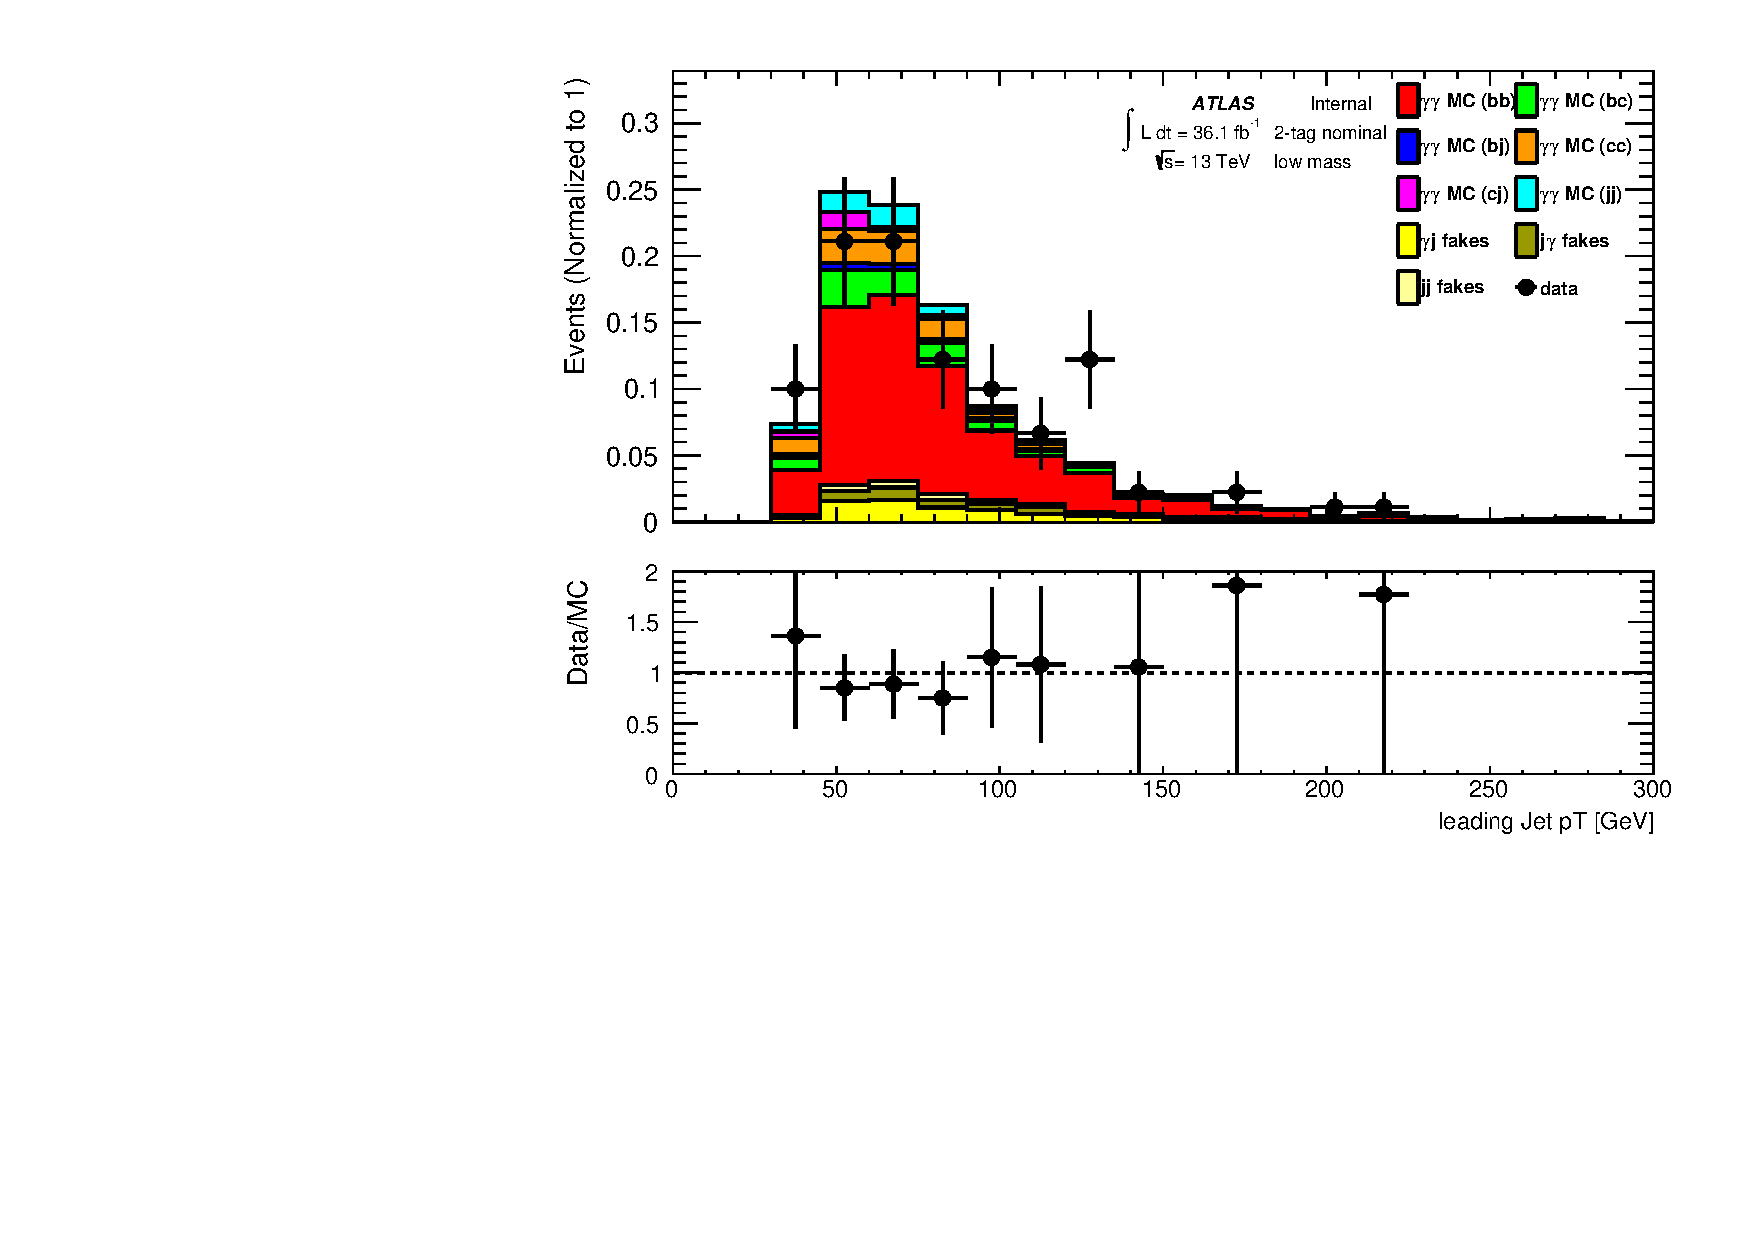
\includegraphics[width=0.48\textwidth]{chapters/chapter5_yybb/images/data_MC_comparison/h_SR_l_2t_nominal_leadingJet_pt.pdf}
  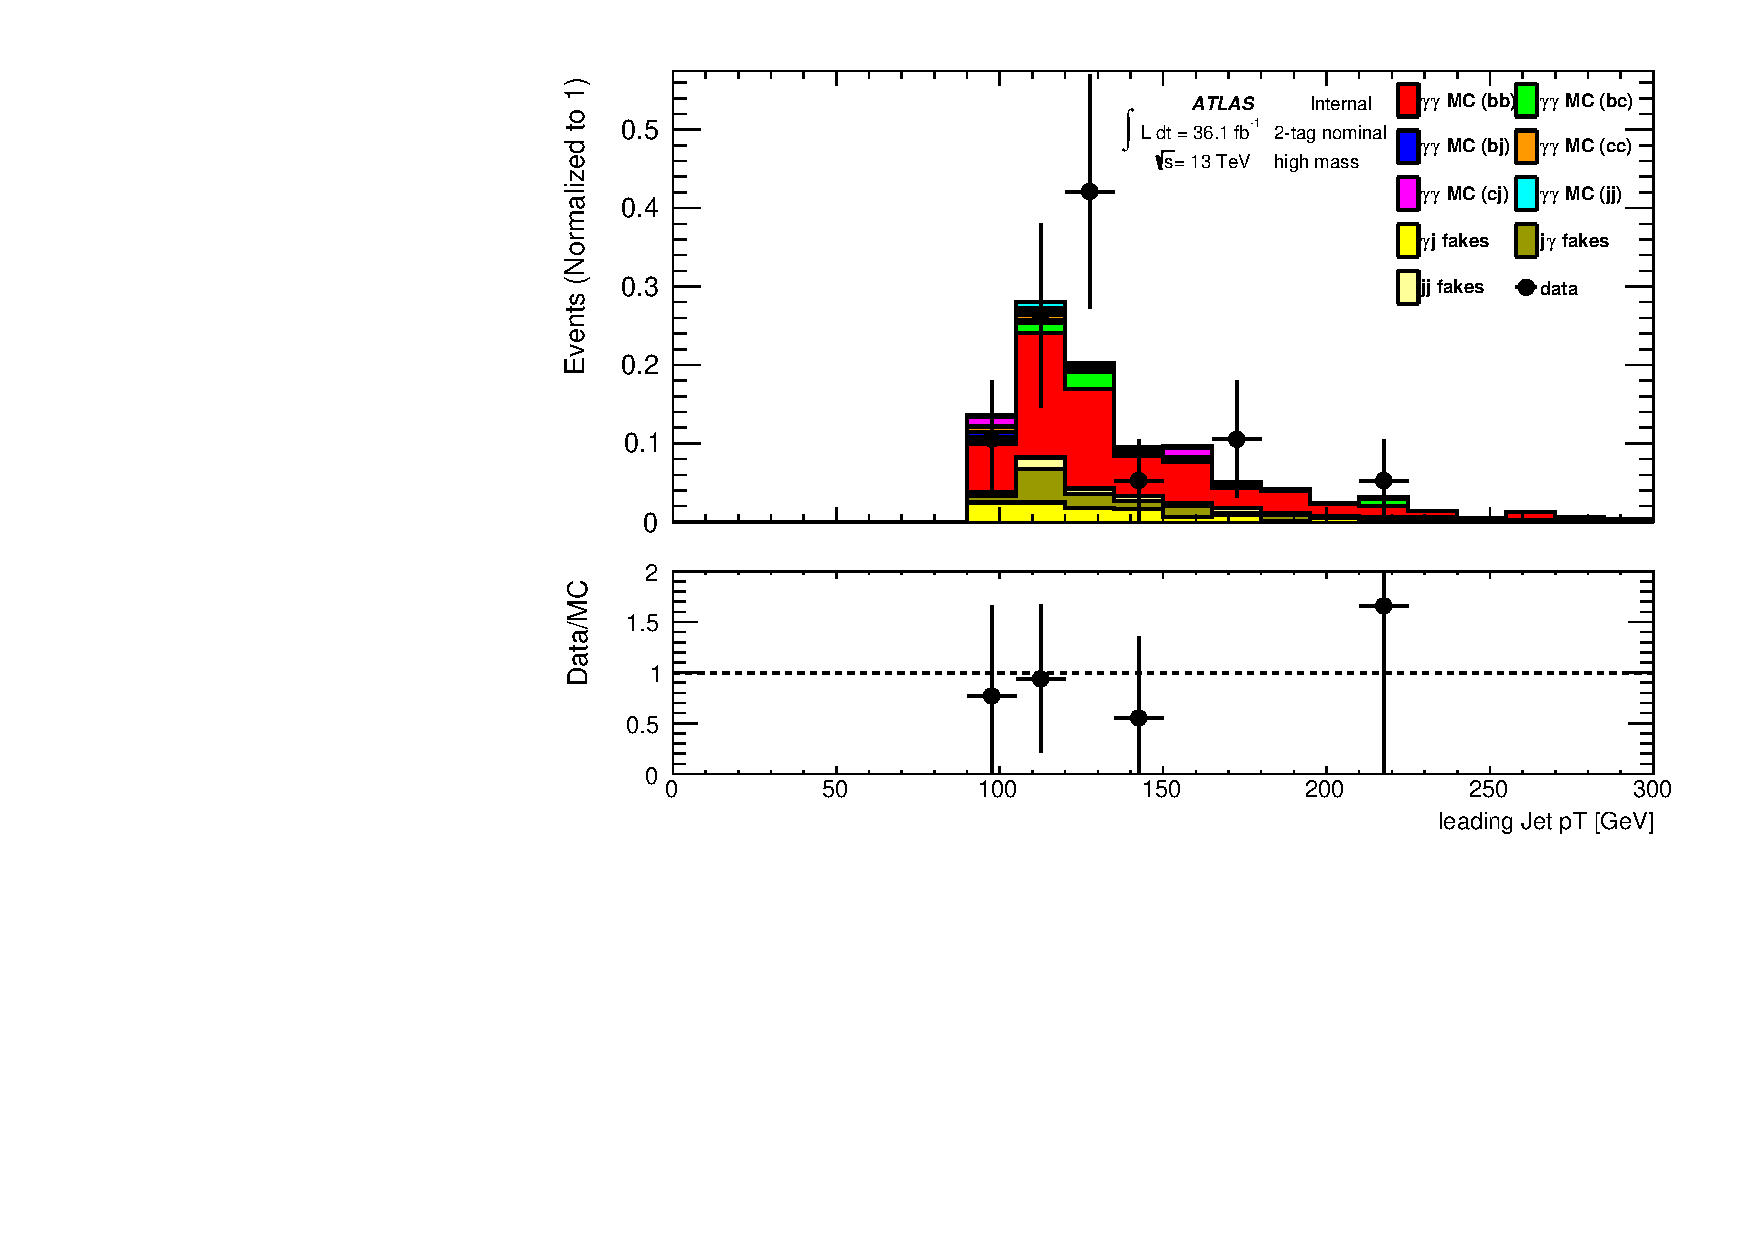
\includegraphics[width=0.48\textwidth]{chapters/chapter5_yybb/images/data_MC_comparison/h_SR_h_2t_nominal_leadingJet_pt.pdf}
  \caption[Leading jet \pt.]{Leading jet \pt by b-tagging category. The low (left) and high (right) mass selections are shown. Both data and MC are normalized such that the integral is 1.
  \label{fig:jet_l_pt}}
\end{figure}

\begin{figure}[p]
  \centering
  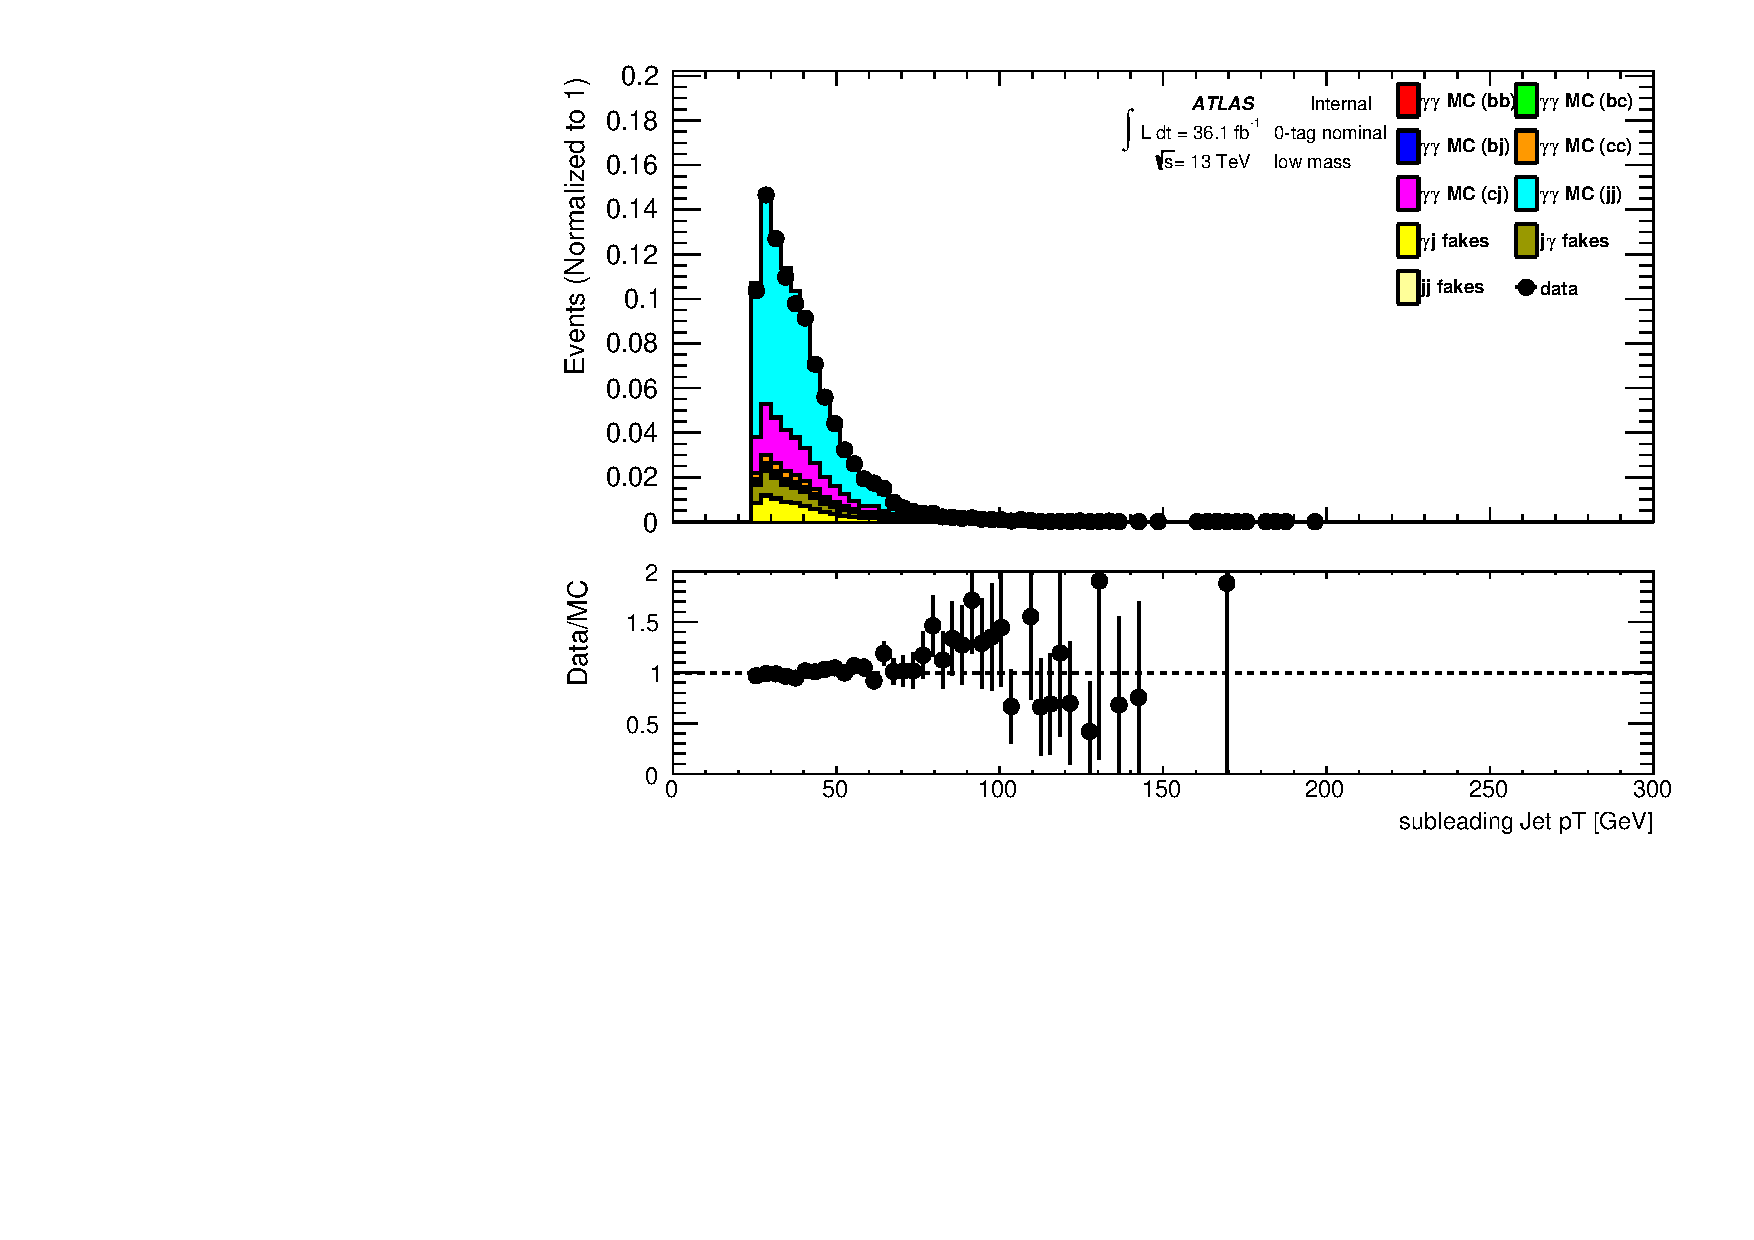
\includegraphics[width=0.48\textwidth]{chapters/chapter5_yybb/images/data_MC_comparison/h_CR_l_0t_nominal_subleadingJet_pt.pdf}
  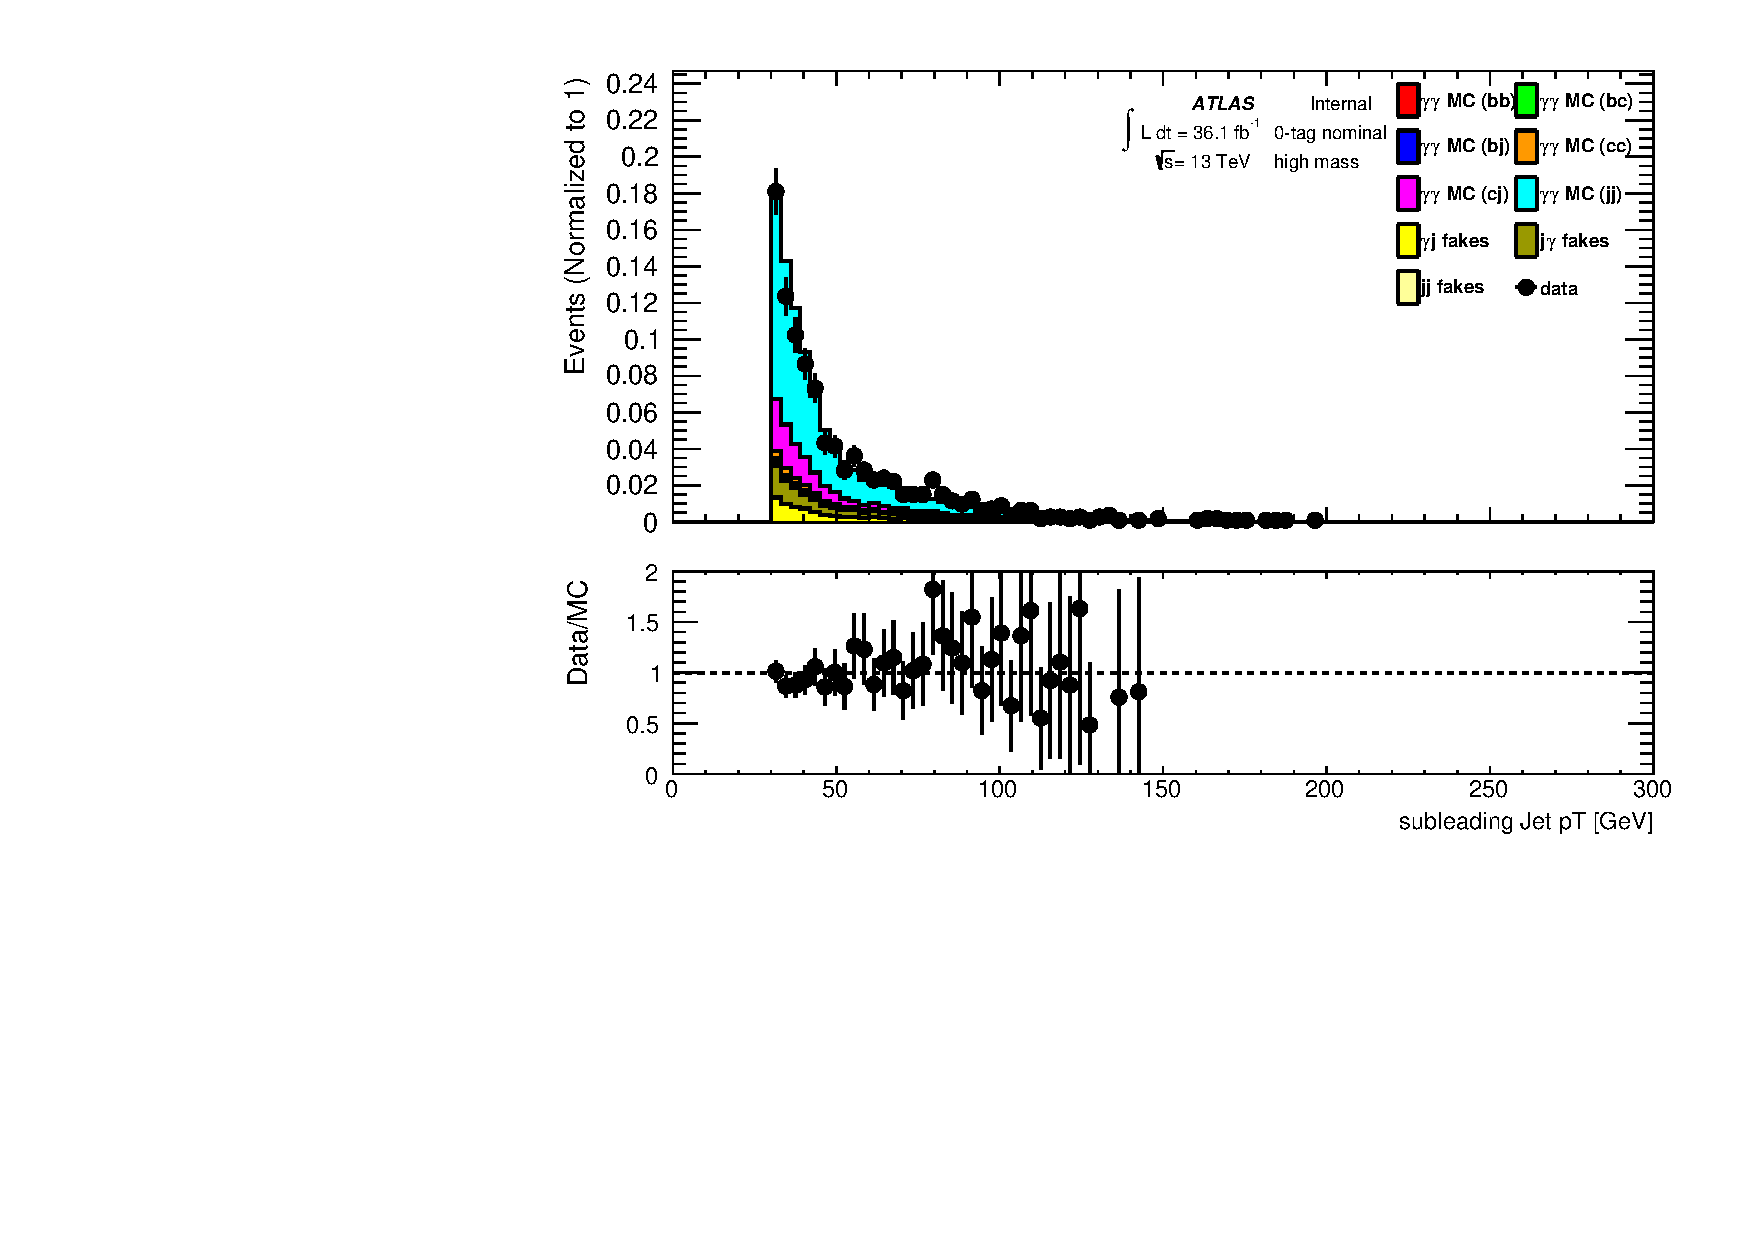
\includegraphics[width=0.48\textwidth]{chapters/chapter5_yybb/images/data_MC_comparison/h_CR_h_0t_nominal_subleadingJet_pt.pdf}
  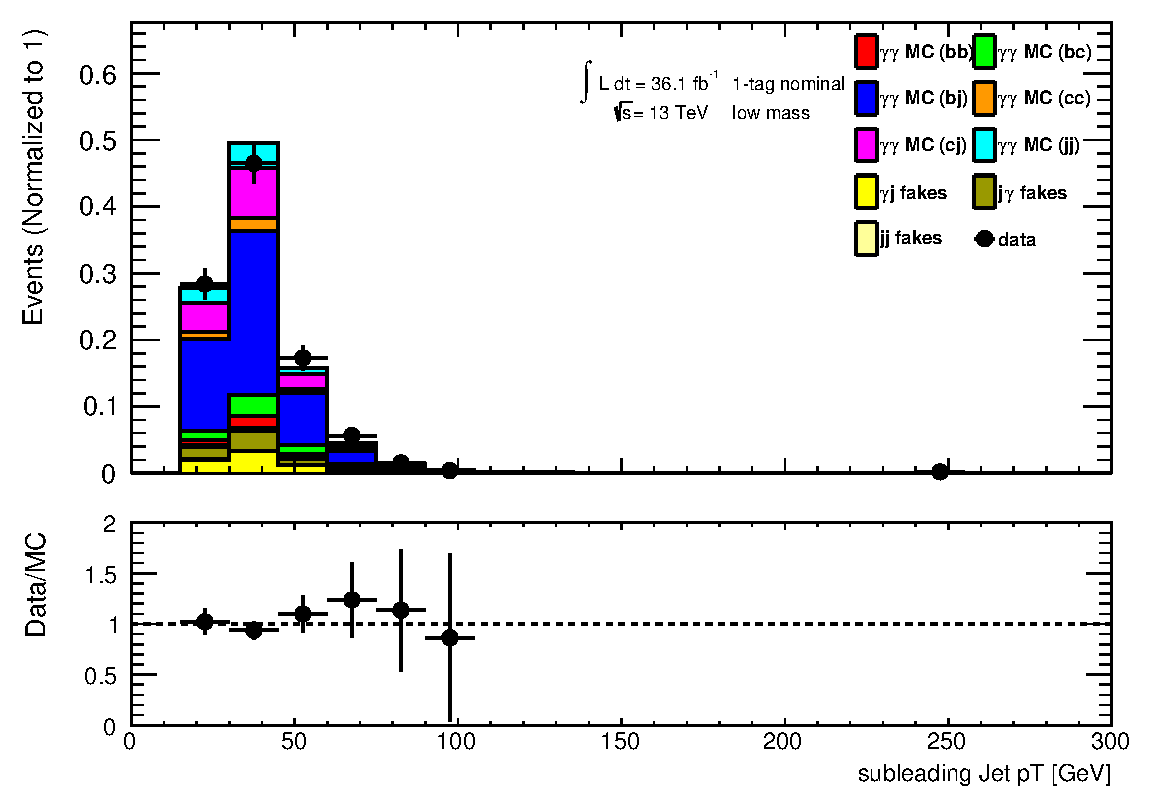
\includegraphics[width=0.48\textwidth]{chapters/chapter5_yybb/images/data_MC_comparison/h_SR_l_1t_nominal_subleadingJet_pt.pdf}
  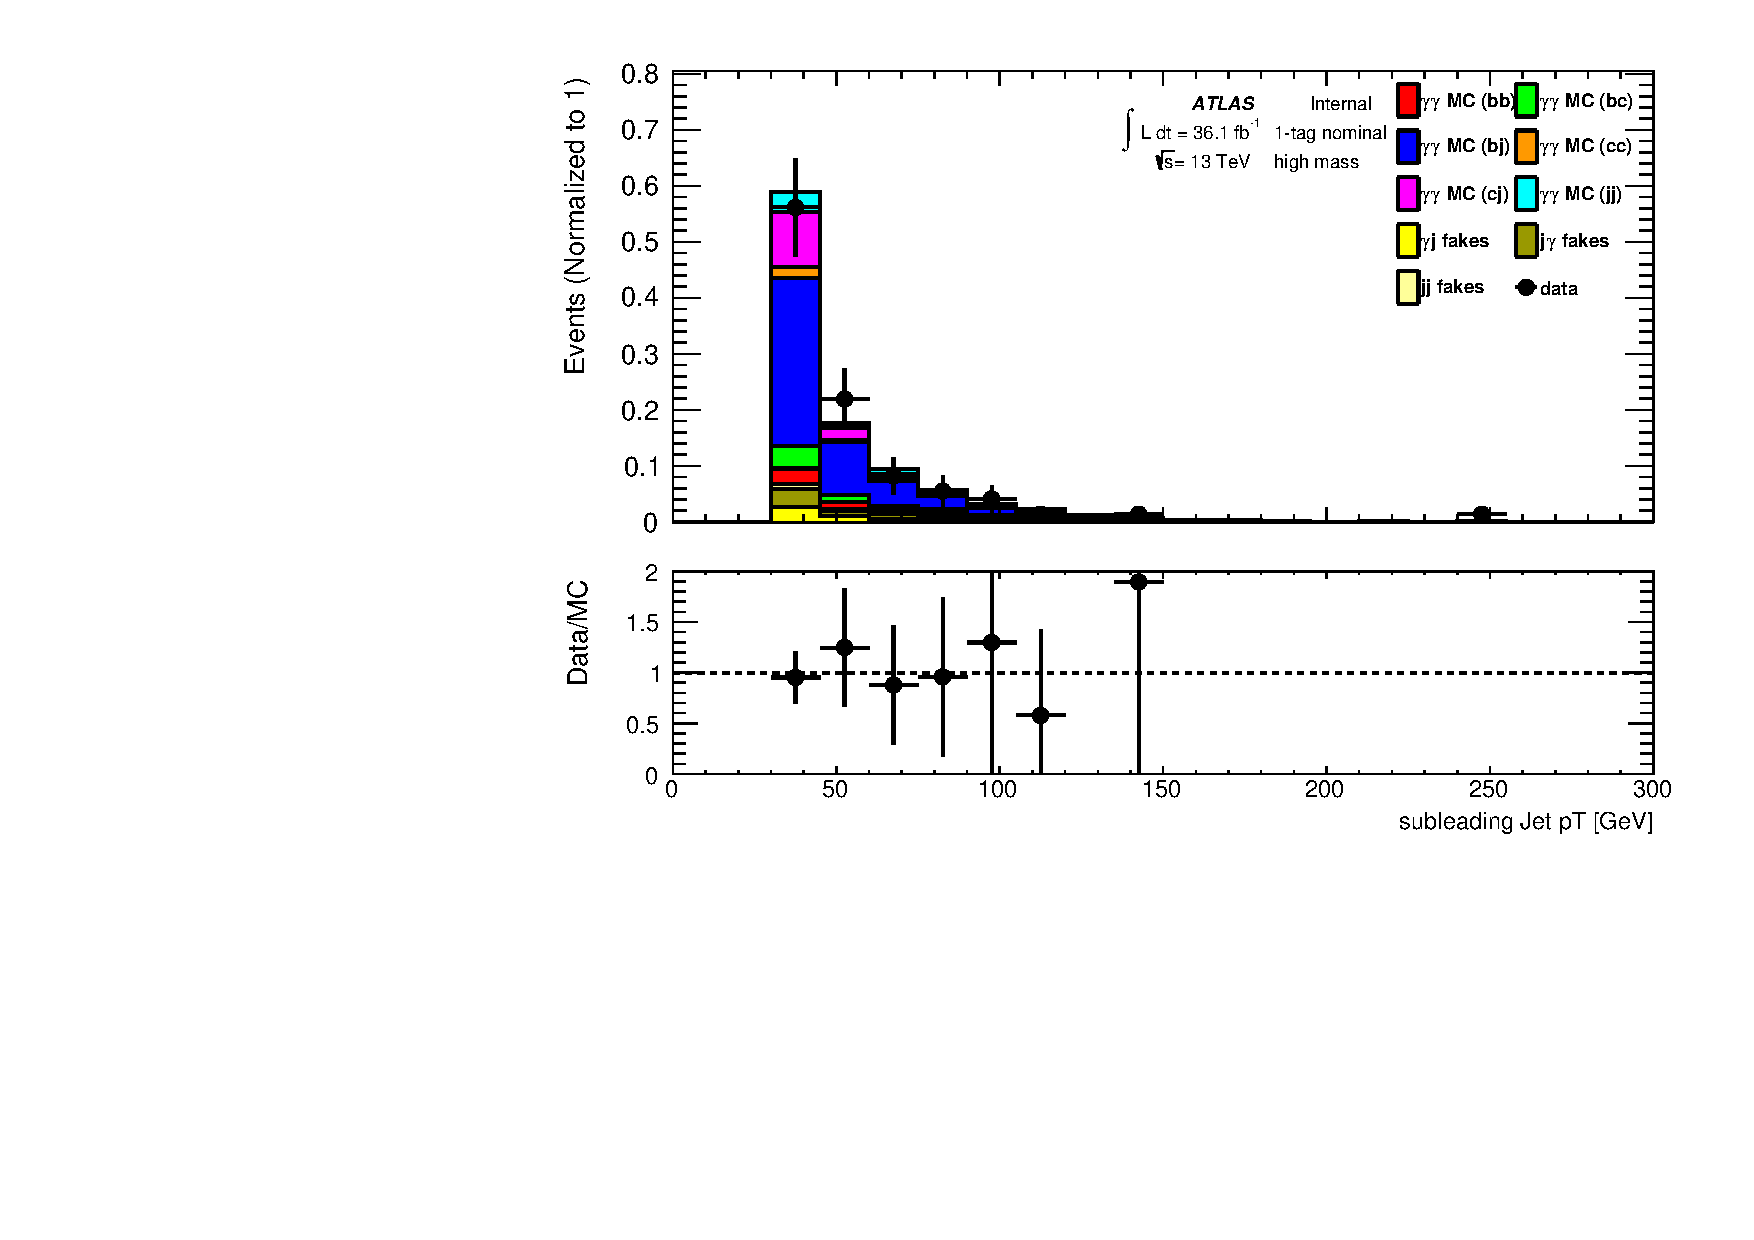
\includegraphics[width=0.48\textwidth]{chapters/chapter5_yybb/images/data_MC_comparison/h_SR_h_1t_nominal_subleadingJet_pt.pdf}
  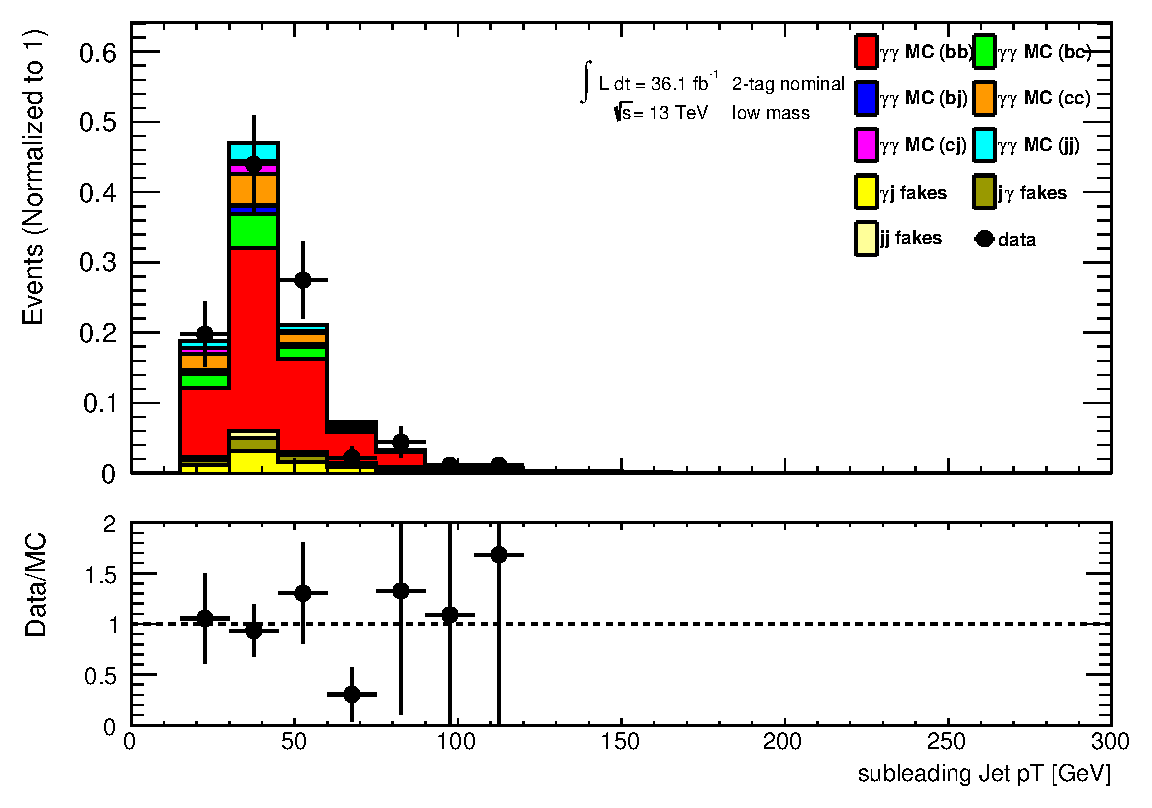
\includegraphics[width=0.48\textwidth]{chapters/chapter5_yybb/images/data_MC_comparison/h_SR_l_2t_nominal_subleadingJet_pt.pdf}
  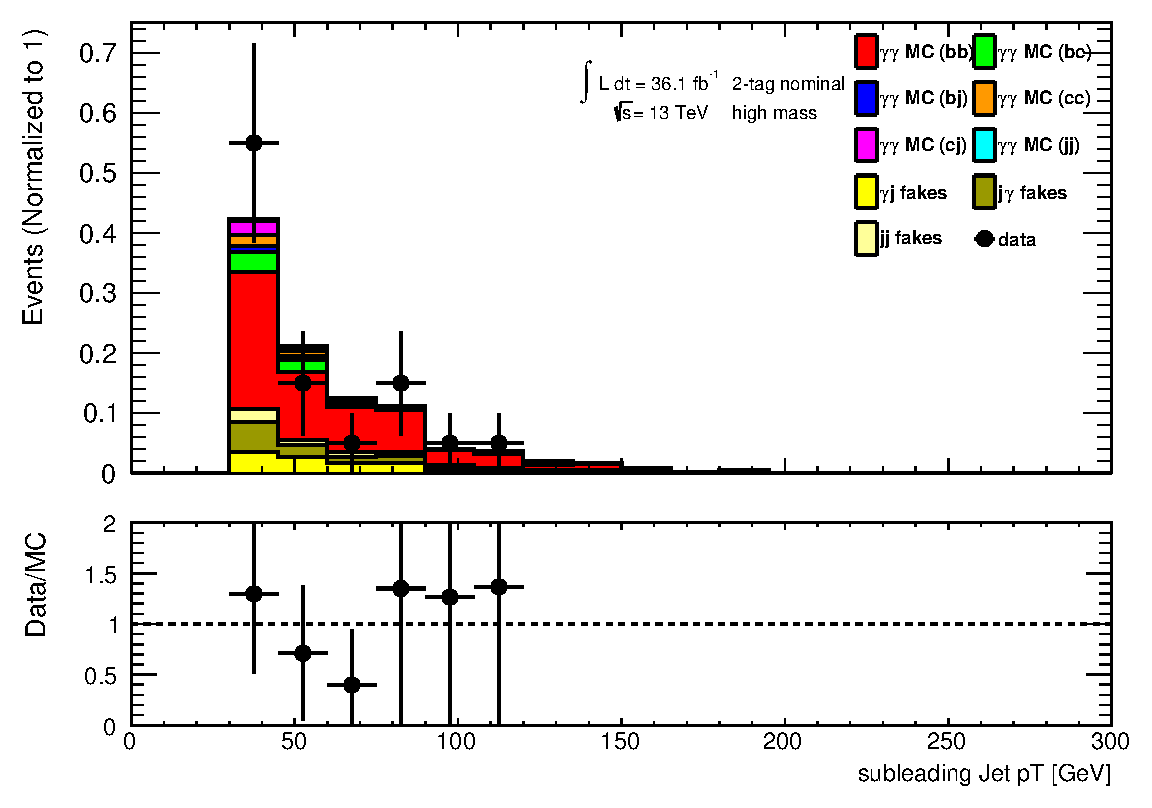
\includegraphics[width=0.48\textwidth]{chapters/chapter5_yybb/images/data_MC_comparison/h_SR_h_2t_nominal_subleadingJet_pt.pdf}
  \caption[Subleading jet \pt.]{Leading jet \pt by b-tagging category. The low (left) and high (right) mass selections are shown. Both data and MC are normalized such that the integral is 1.
  \label{fig:jet_s_pt}}
\end{figure}


In order to reconstruct the 4-body mass, $m_{\gamma\gamma jj}$, in cases where there are not 2 $b$-tagged jets, an additional candidate jet is selected through the use of a \gls{BDT}. The inputs to this \gls{BDT} are: jet and dijet \pt, dijet mass, jet and dijet $\eta$, dijet \Deta, booleans for passing the 77\% and 85\% \btagging WP, and the ranking of the jets in terms of:

\begin{itemize}
  \item Highest jet \pt
  \item Lowest $\Delta m = m_{bb} - m_H$ when summed with the $b$-tagged jet
  \item Highest dijet \pt, when summed with the $b$-tagged jet
\end{itemize}

The jet with the highest \gls{BDT} score is selected as the pairing when constructing  $m_{\gamma\gamma jj}$. The performance is better at high mass hypotheses, since the signal shape is more pronounced from the background than at low masses. 

% TODO: ADD plots

\subsection{Electrons}

Electrons are used to reject jets originating from leptons. Electrons are required to have $\pt > \unit{10}{\GeV}$, and $\abseta < 2.47$ and outside of the crack-region ($1.37 < \abseta < 1.52$). They must pass medium identification and loose isolation requirements, which are set on both calorimeter and tracking variables and are 99\% efficient.

\subsection{Muons}

In jet reconstruction, a muon-in-jet correction is used to improve resolution for $b$-jets. This accounts for leptonic decays involving muons which do not entirely deposit their energy in the \gls{EM} calorimeter. Muons must pass medium requirements, have $\pt > \unit{4}{\GeV}$, $\abseta < 2.7$, $|d_{0}|$ significance less than 3, $|z_{0}|$ less than 0.5 mm\footnote{Both $|d_{0}|$ and $|z_{0}|$ requirements are with respect to the primary vertex.}.

For correcting the $b$-jets, the 4-momenta of all muons within the jet's \Dr cone are added to the $b$-jet. Adding this correction shifts the $m_{bb}$ distribution closer to the Higgs mass and provides a $5-6\%$ improvement in signal acceptance for each resonant mass point. Figure \ref{fig:n_muons} shows the number of muons added to each jet, typically 0 or 1 muon.

\begin{figure}[!ht]
  \centering
  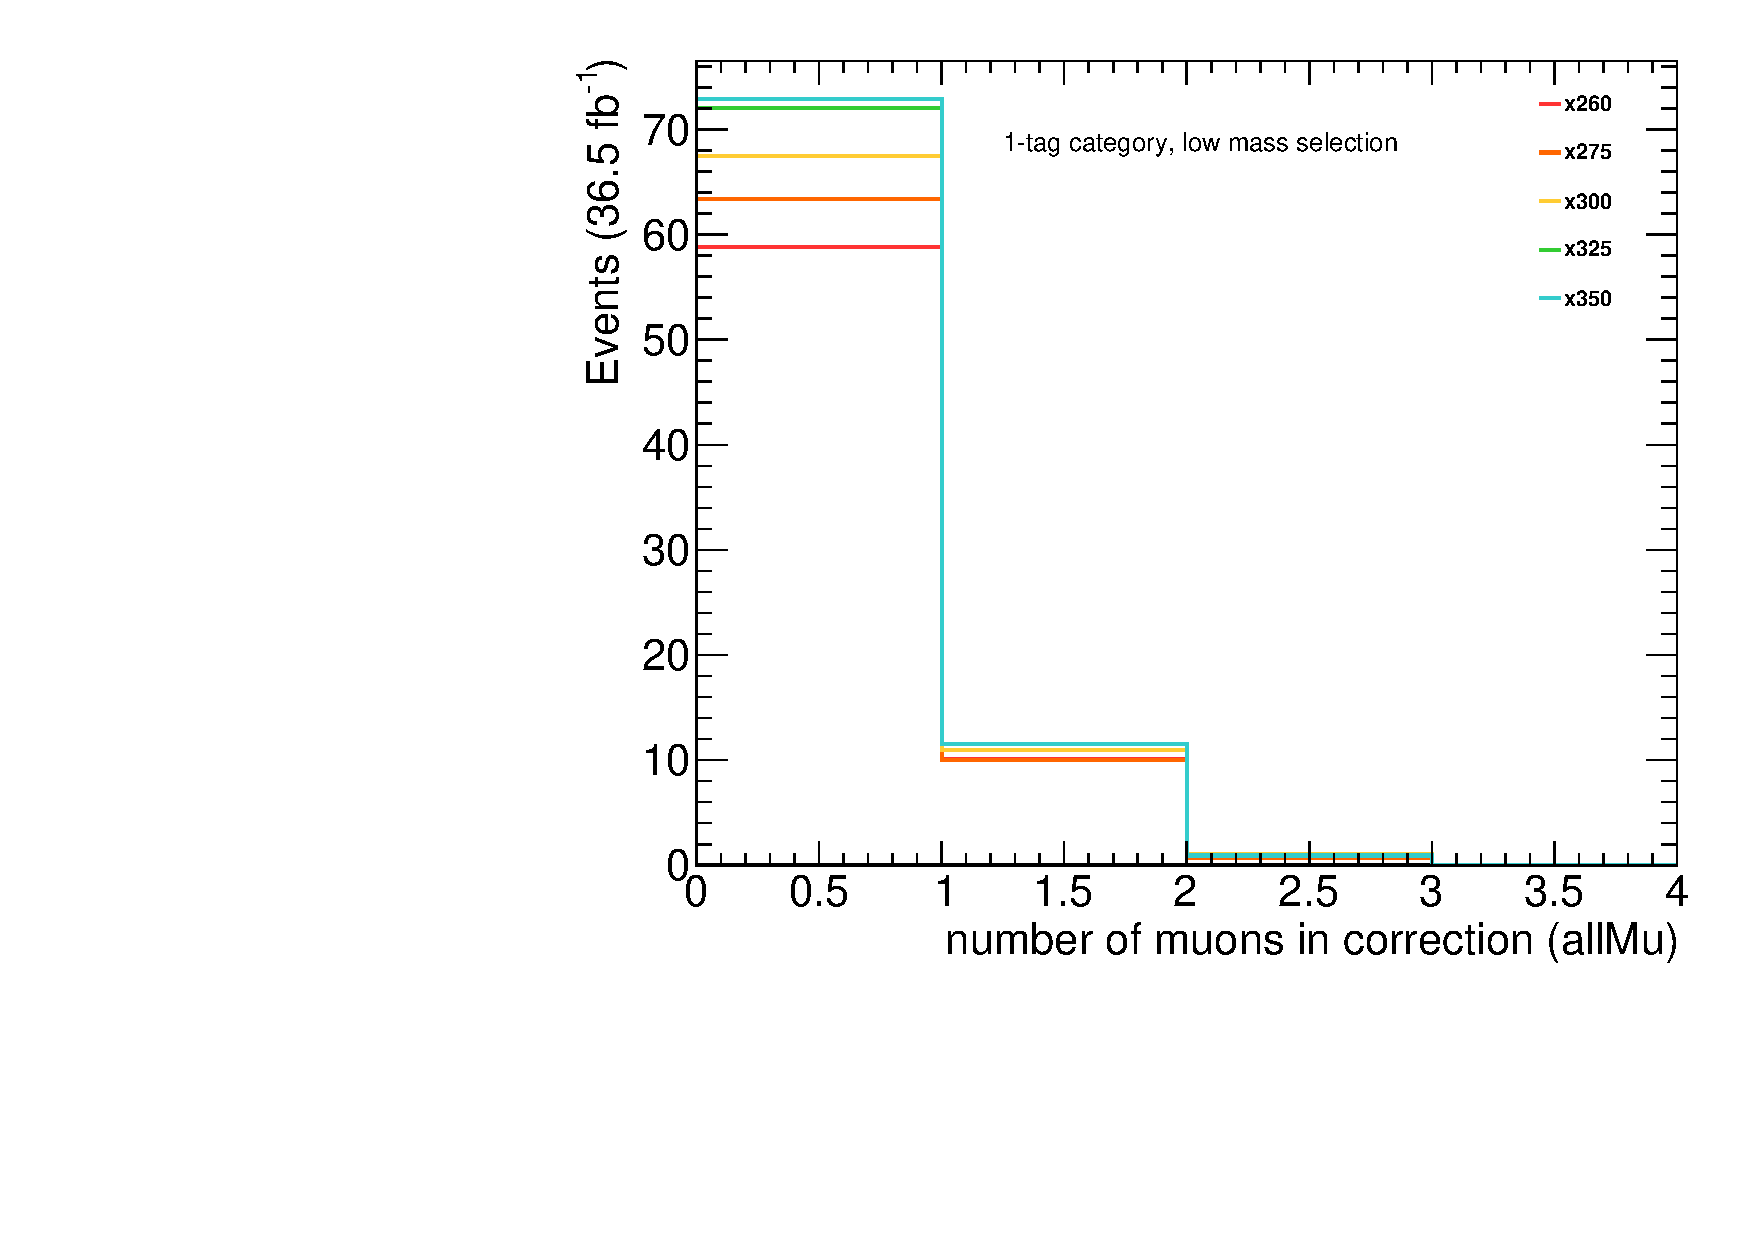
\includegraphics[height=0.32\textwidth]{chapters/chapter5_yybb/images/muon-in-jet/all_mu_n_allMu_low_1.pdf}
  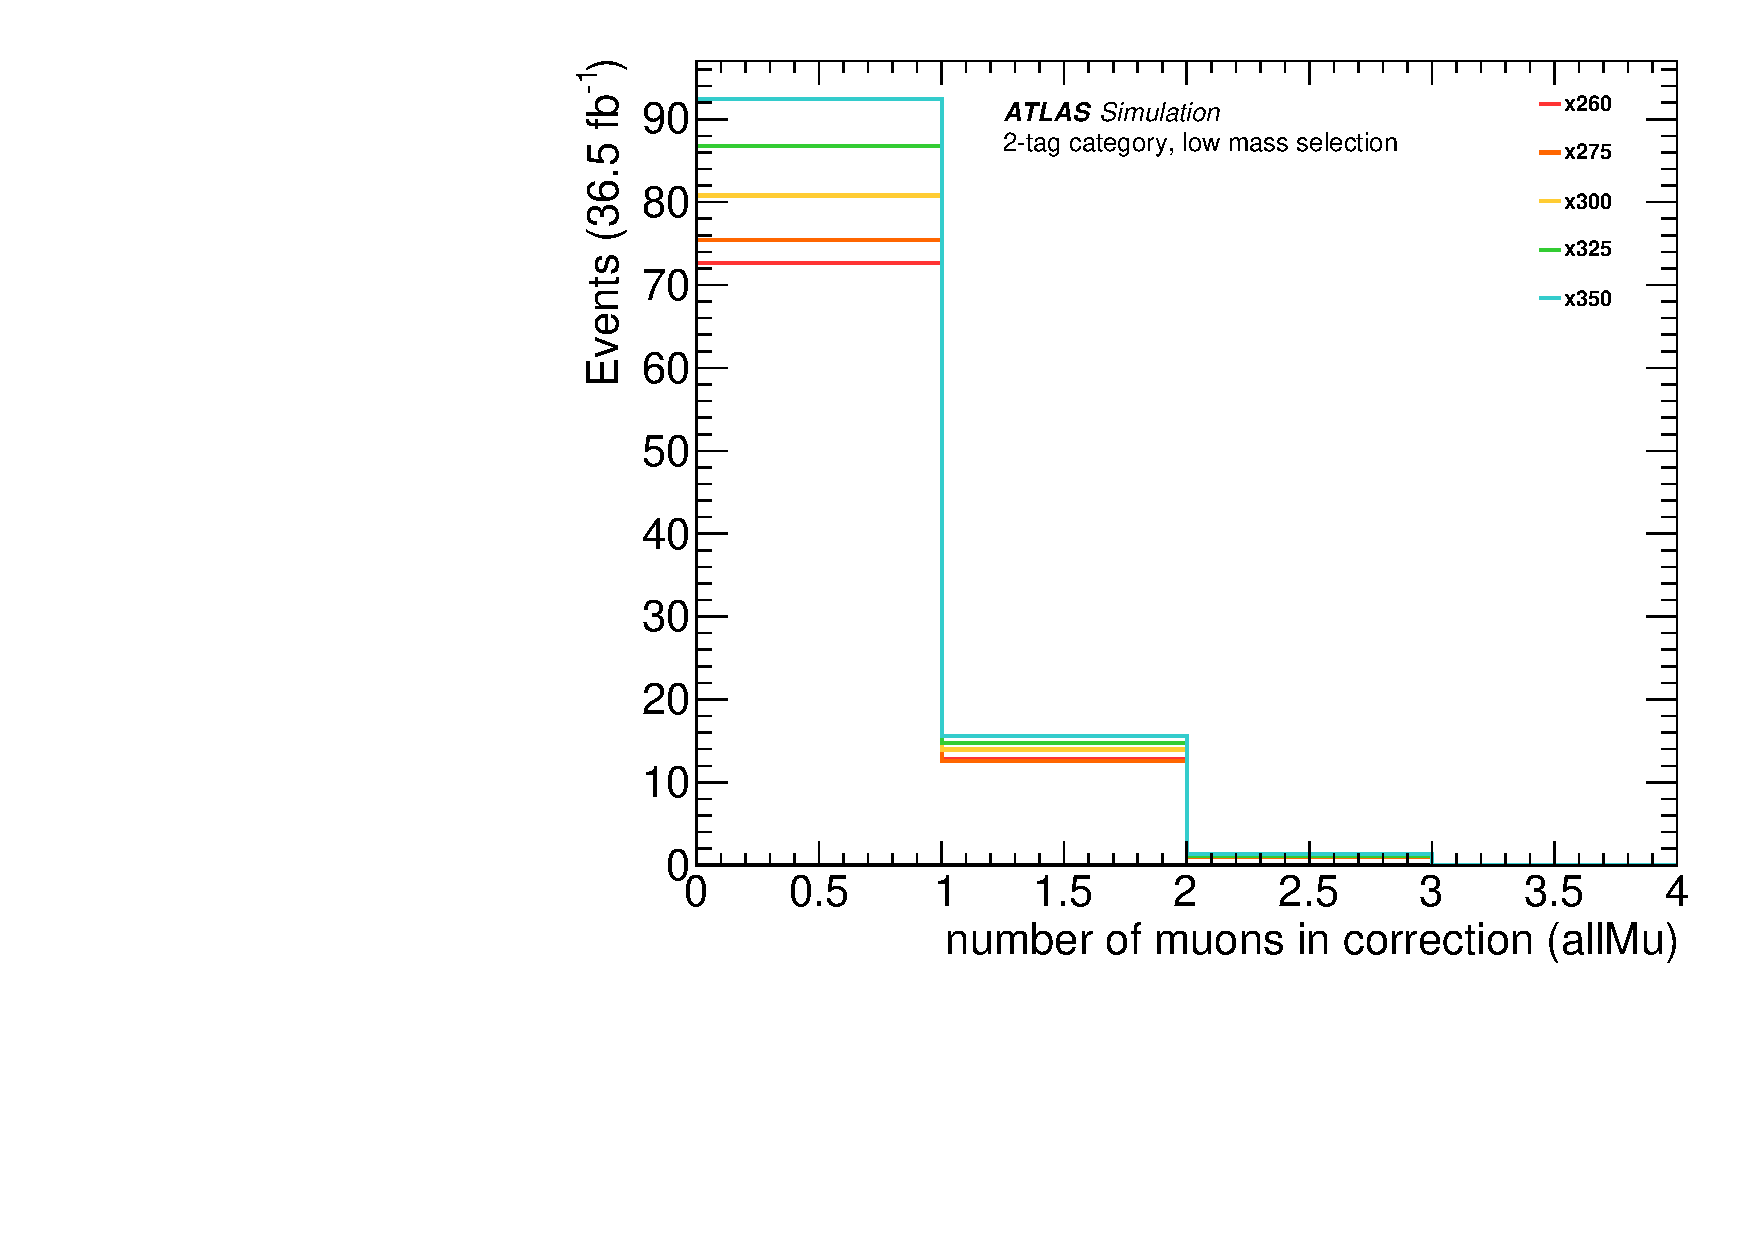
\includegraphics[height=0.32\textwidth]{chapters/chapter5_yybb/images/muon-in-jet/all_mu_n_allMu_low_2.pdf} \\
  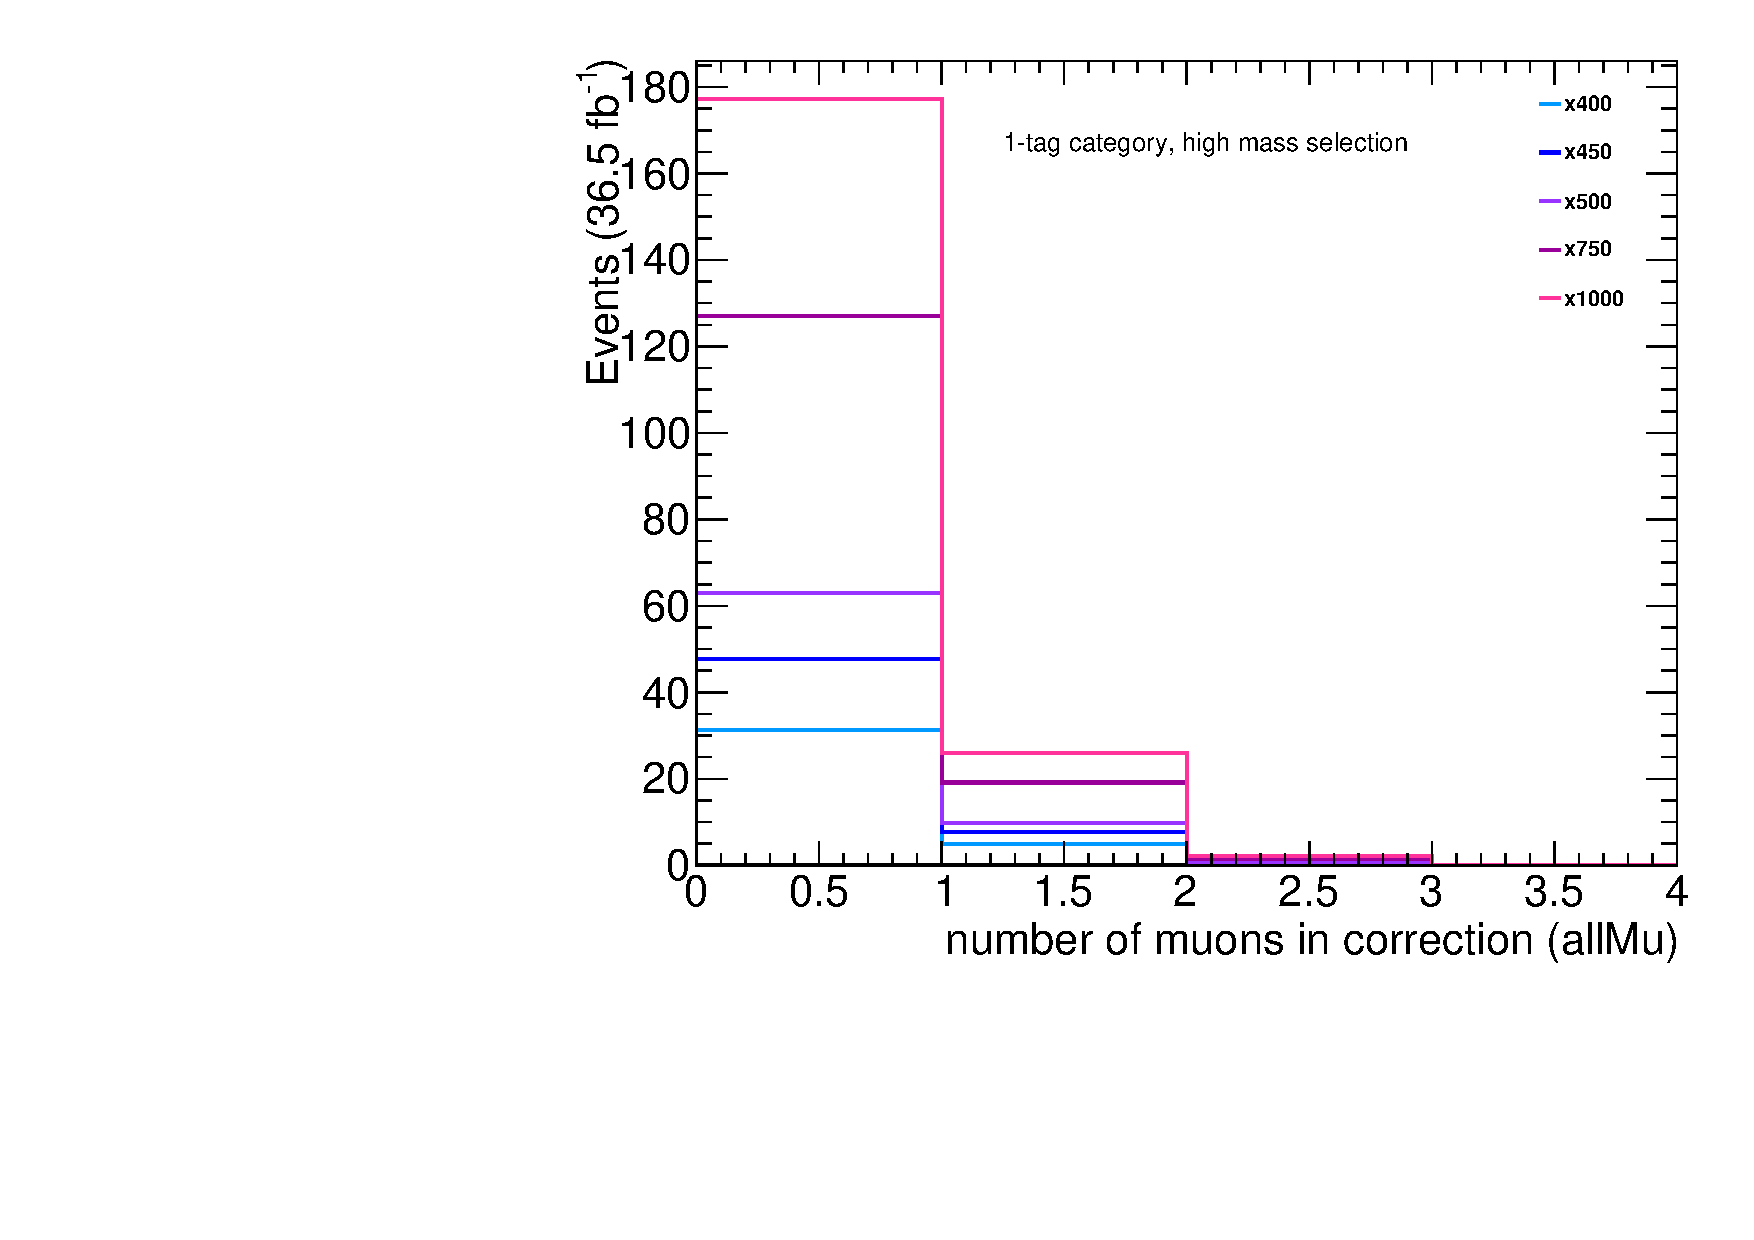
\includegraphics[height=0.32\textwidth]{chapters/chapter5_yybb/images/muon-in-jet/all_mu_n_allMu_high_1.pdf}
  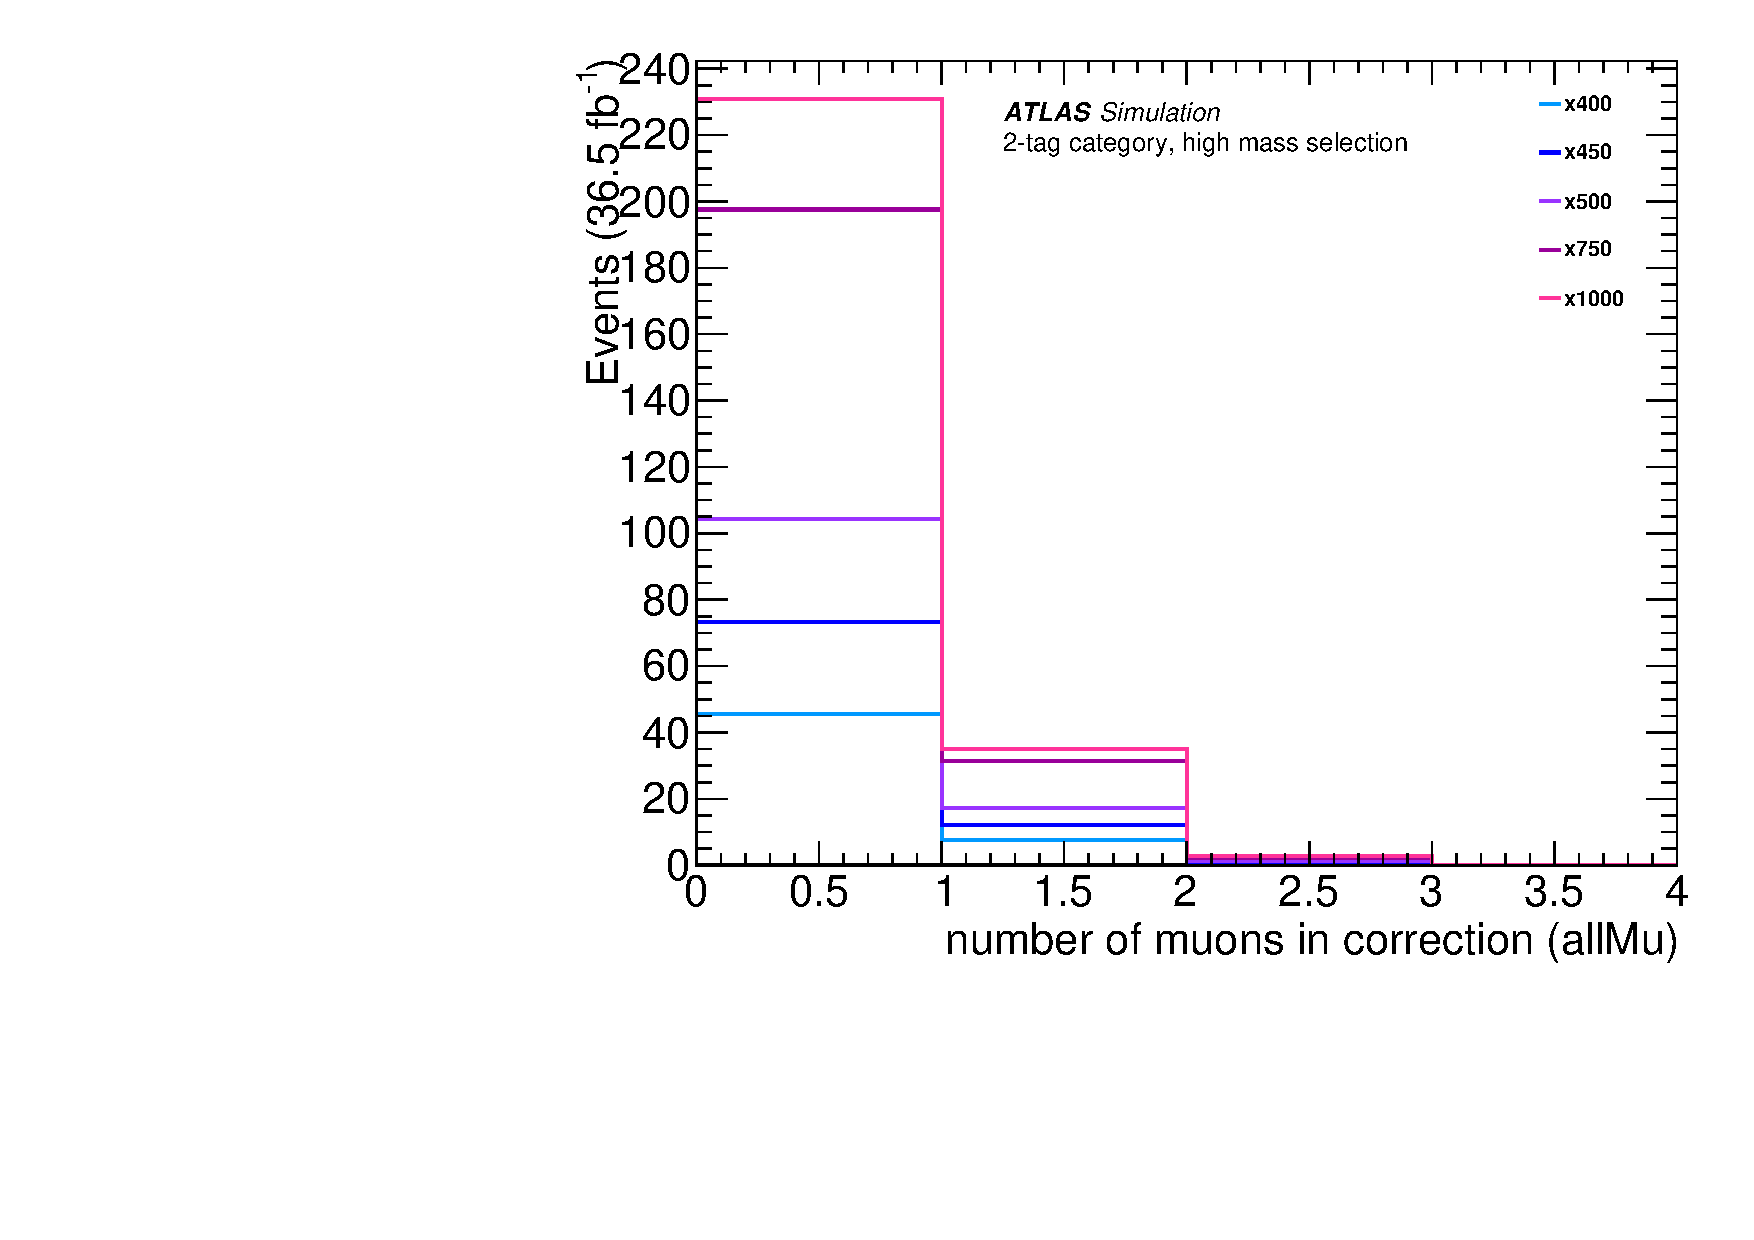
\includegraphics[height=0.32\textwidth]{chapters/chapter5_yybb/images/muon-in-jet/all_mu_n_allMu_high_2.pdf} \\
  \caption[Number of muons added to each jet, shown for each $b$-tagging category with the low and high mass  selections applied]{Number of muons added to each jet, shown for each $b$-tagging category with the low and high mass  selections applied.}
  \label{fig:n_muons}
\end{figure}


\section{Event Selection} \label{sec:yybb-event-selection}
\noindent\textbf{Preselection}\\
\indent For all samples, a preselection common to all \Hgg analyses is applied \cite{hgam-preselection}. To target this decay, events must pass the diphoton trigger, which requires two photons passing \textit{loose} identification. One of these photons must have $\et > \unit{35}{\GeV}$ and the other must have $\et > \unit{25}{\GeV}$. Nominally, this is the \path{g35_loose_g25_loose} trigger. After this trigger requirement, \pt cuts are applied, requiring the leading (subleading) photon \pt to be greater than 35\% (25\%) the diphoton invariant mass. Additionally the diphoton invariant mass must be in the window of 105 to 160 GeV.

\noindent\textbf{Signal Selection}\\
\indent In addition to the preselection requirements, a further requirement of two jets within the \btagging region ($\abseta <2.5$) is added to the preselection in order to target the \Hbb decay. Events are separated into 0, 1, and 2-tag regions based on \btagging criteria. Events with 3 jets passing the 70\% efficient \btagging \gls{WP} are vetoed from this analysis in order to maintain orthogonality with the $HH \rightarrow \bb \bb$ analysis. The 2-tag signal region requires exactly two jets passing the 70\% efficient \btagging \gls{WP}. If an event fails this requirement, but has one \bjet passing the 60\% efficient \btagging \gls{WP}, it is added to the 1-tag signal region. If it fails both of these criteria The 1 and 2-tag regions are used as signal regions, the 0-tag is used as a control region. This logic flow is shown in Figure \ref{fig:btag-logic}.


\tikzstyle{startstop} = [rectangle, rounded corners, minimum width=3cm, minimum height=1cm,text centered, draw=black, fill=orange!30]
\tikzstyle{io} = [rectangle, rounded corners, minimum width=3cm, minimum height=1cm,text centered, draw=black, fill=blue!30]
\tikzstyle{rej} = [rectangle, rounded corners, minimum width=3cm, minimum height=1cm,text centered, draw=black, fill=red!30]
\tikzstyle{decision} = [diamond, minimum width=3cm, minimum height=1cm, text centered, draw=black, fill=green!30]
\tikzstyle{arrow} = [thick,->,>=stealth]
\begin{figure}[htbp]
  \centering
  \begin{tikzpicture}[node distance=3cm]
    \node (start) [startstop] {Start};
  
    \node (dec1) [decision, below of=start] {$n_{b,70\%} >2$};
    \node (out1) [rej, right of=dec1, xshift=2cm] {Veto};
  
    \node (dec2) [decision, below of=dec1, yshift=-1cm] {$n_{b,70\%} = 2$};
    \node (out2) [io, right of=dec2, xshift=2cm] {2-tag Category};
  
    \node (dec3) [decision, below of=dec2, yshift=-1cm] {$n_{b,60\%} = 1$};
    \node (out3) [io, right of=dec3, xshift=2cm] {1-tag Category};
    \node (out4) [io, below of=dec3] {0-tag Category};

    \draw [arrow] (start) -- (dec1);
    
    \draw [arrow] (dec1) -- node[anchor=north] {True} (out1);
    \draw [arrow] (dec1) -- node[anchor=west] {False} (dec2);

    \draw [arrow] (dec2) -- node[anchor=north] {True} (out2);
    \draw [arrow] (dec2) -- node[anchor=west] {False} (dec3);    
    
    \draw [arrow] (dec3) -- node[anchor=north] {True} (out3);
    \draw [arrow] (dec3) -- node[anchor=west] {False} (out4);  
  
  \end{tikzpicture}
  \caption[Logic flowchart for analysis b-tagging category definitions]{Logic flowchart for analysis b-tagging category definitions. The 1 and 2-tag categories are signal regions, the 0-tag category is a control region. Events with more than 2 b-tagged jets are rejected to maintain event orthogonality with the $HH\rightarrow \bb\bb$ analysis.}
  \label{fig:btag-logic}
\end{figure}

After selection, overlapping low and high mass selections are created. In the resonant search, the low mass selection is for signal hypotheses of $\unit{500}{\GeV}$ and below; the high mass selection is used for $\unit{500}{\GeV}$ and above. In the non-resonant search, the high mass hypothesis is used. These selections are defined by:

\begin{itemize}
  \item \textbf{Low Mass:} Leading jet $\pt > \unit{40}{\GeV}$, subleading jet $\pt > \unit{25}{\GeV}$, and $80 < m_{bb}/\GeV < 140$
  \item \textbf{High Mass:} Leading jet $\pt > \unit{100}{\GeV}$, subleading jet $\pt > \unit{30}{\GeV}$, and $90 < m_{bb}/\GeV < 140$
\end{itemize}

Due to the poor mass resolution of the \bb system, a scale factor is applied, assuming the decay is consistent with the signal hypothesis, a \gls{SM} Higgs boson. The 4-vector of the system is rescaled by a factor of $m_{H}/\mbb$ (with $m_H \equiv \unit{125.09}{\GeV}$). This scaling improves the \myybb resolution as shown in Figure \ref{fig:resolution-myybb}.


\begin{figure}[!ht]
  \centering
  \subfloat[Low Mass, 1-tag selection]{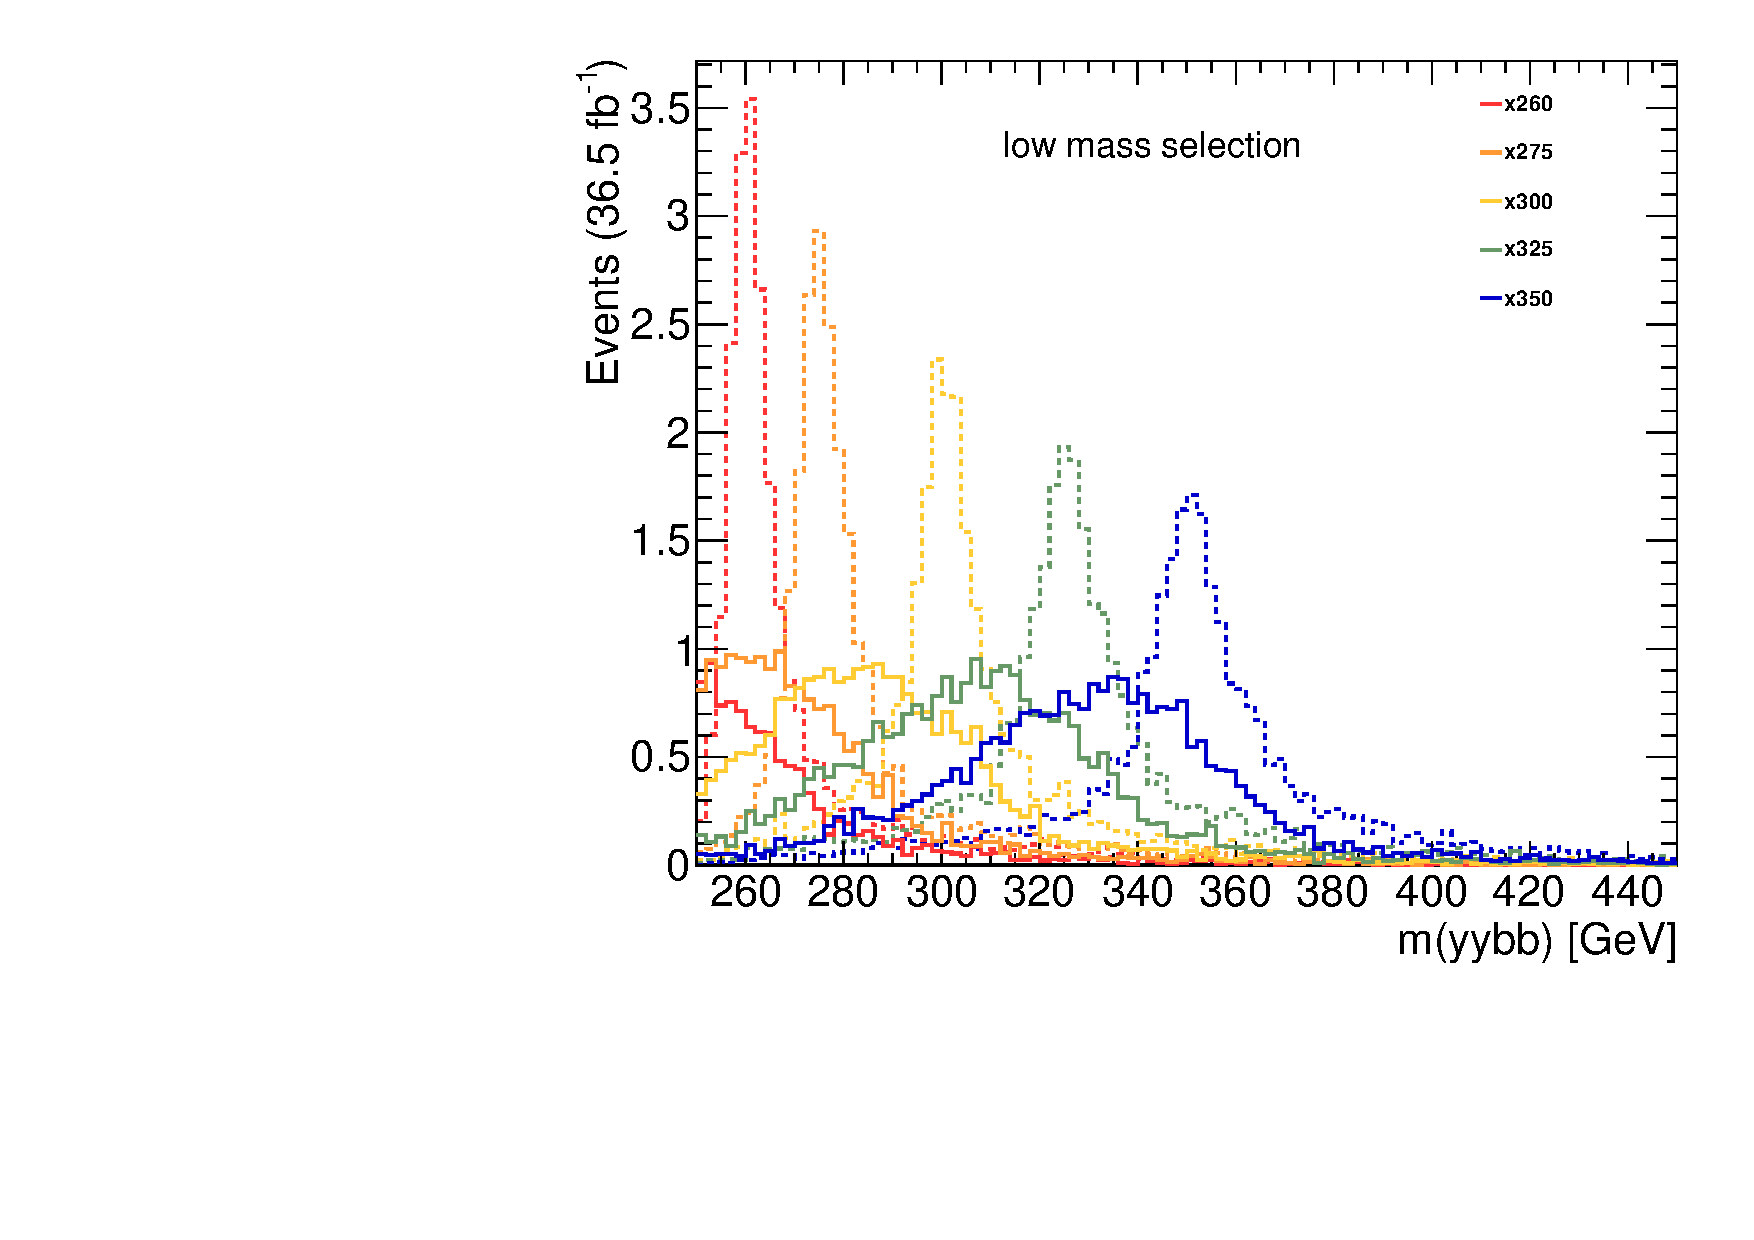
\includegraphics[width=0.48\textwidth]{chapters/chapter5_yybb/images/selection/m_yybb_low_1.pdf}}
  \subfloat[High Mass, 1-tag selection]{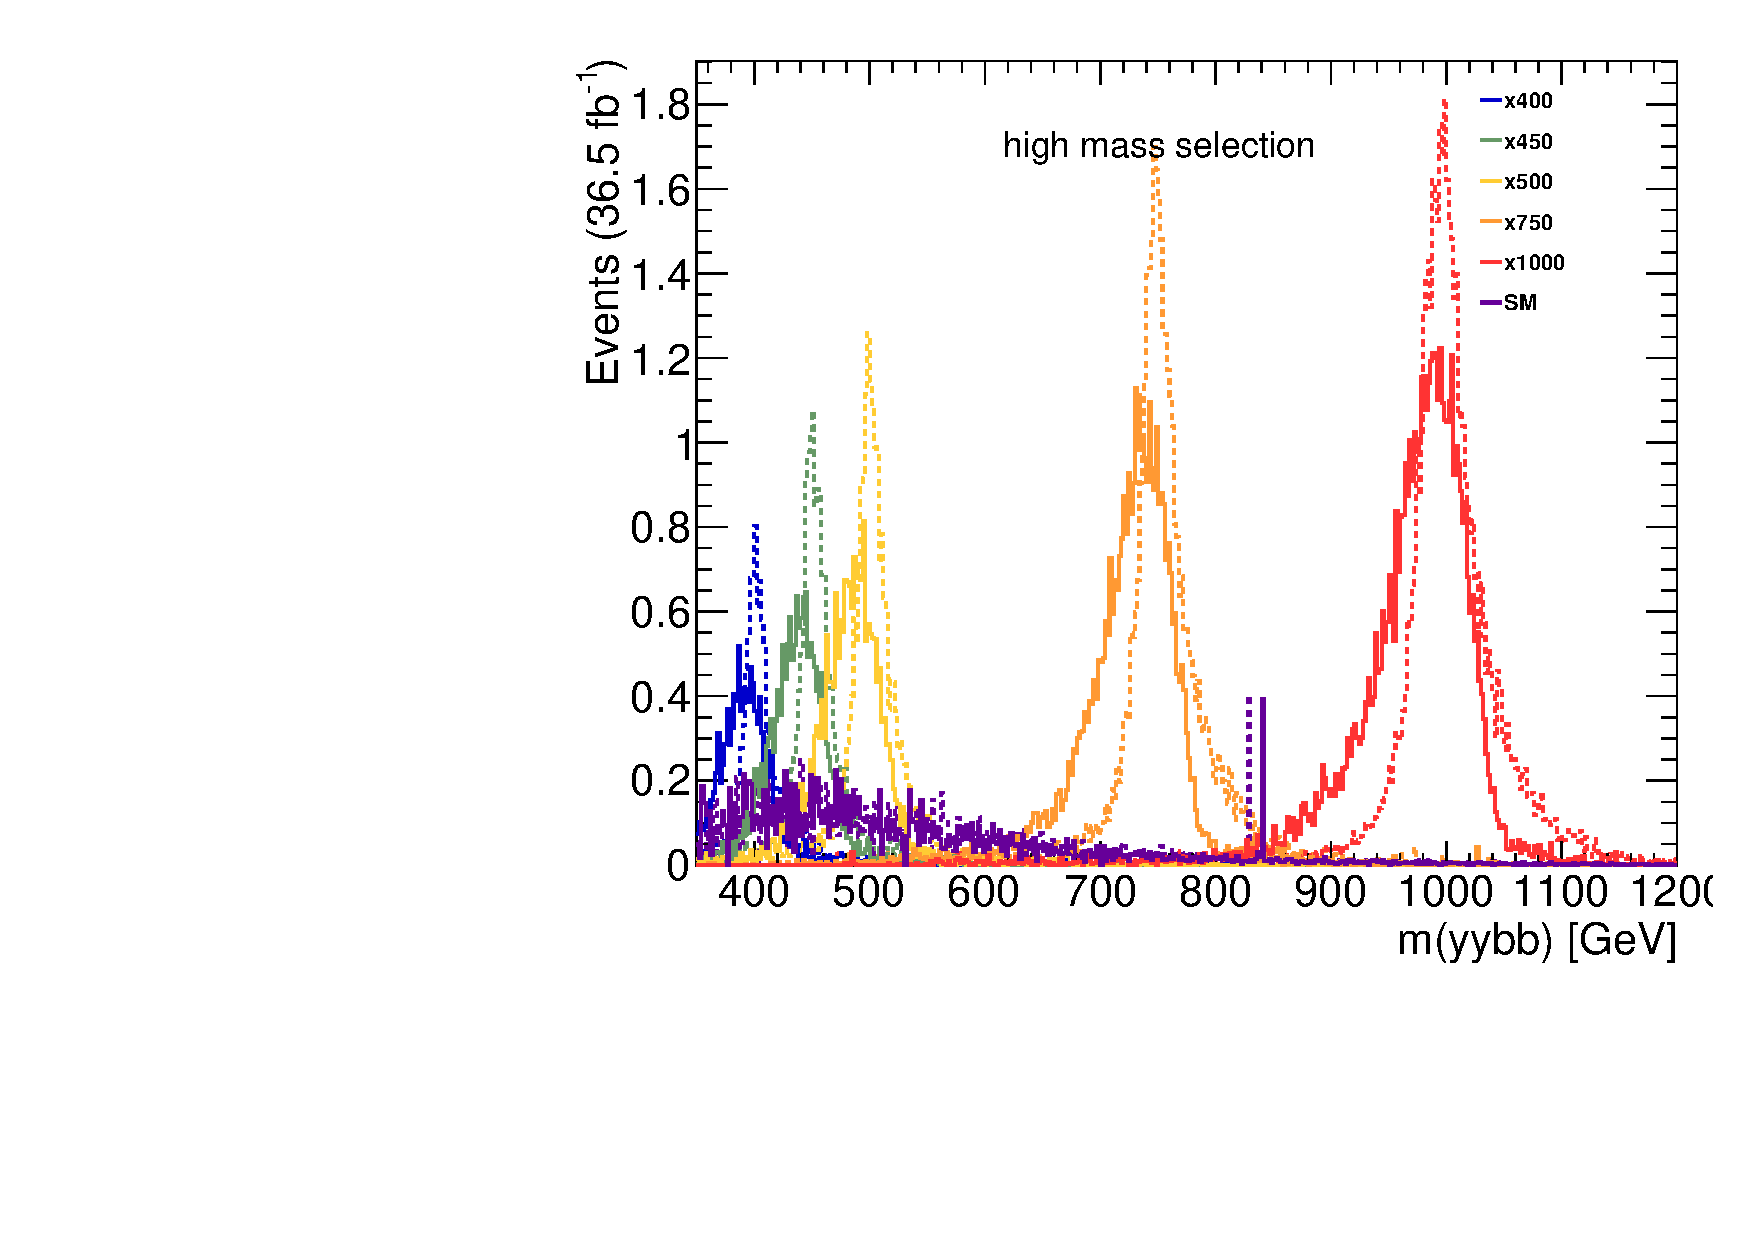
\includegraphics[width=0.48\textwidth]{chapters/chapter5_yybb/images/selection/m_yybb_high_1.pdf}}\\
  \subfloat[Low Mass, 2-tag selection]{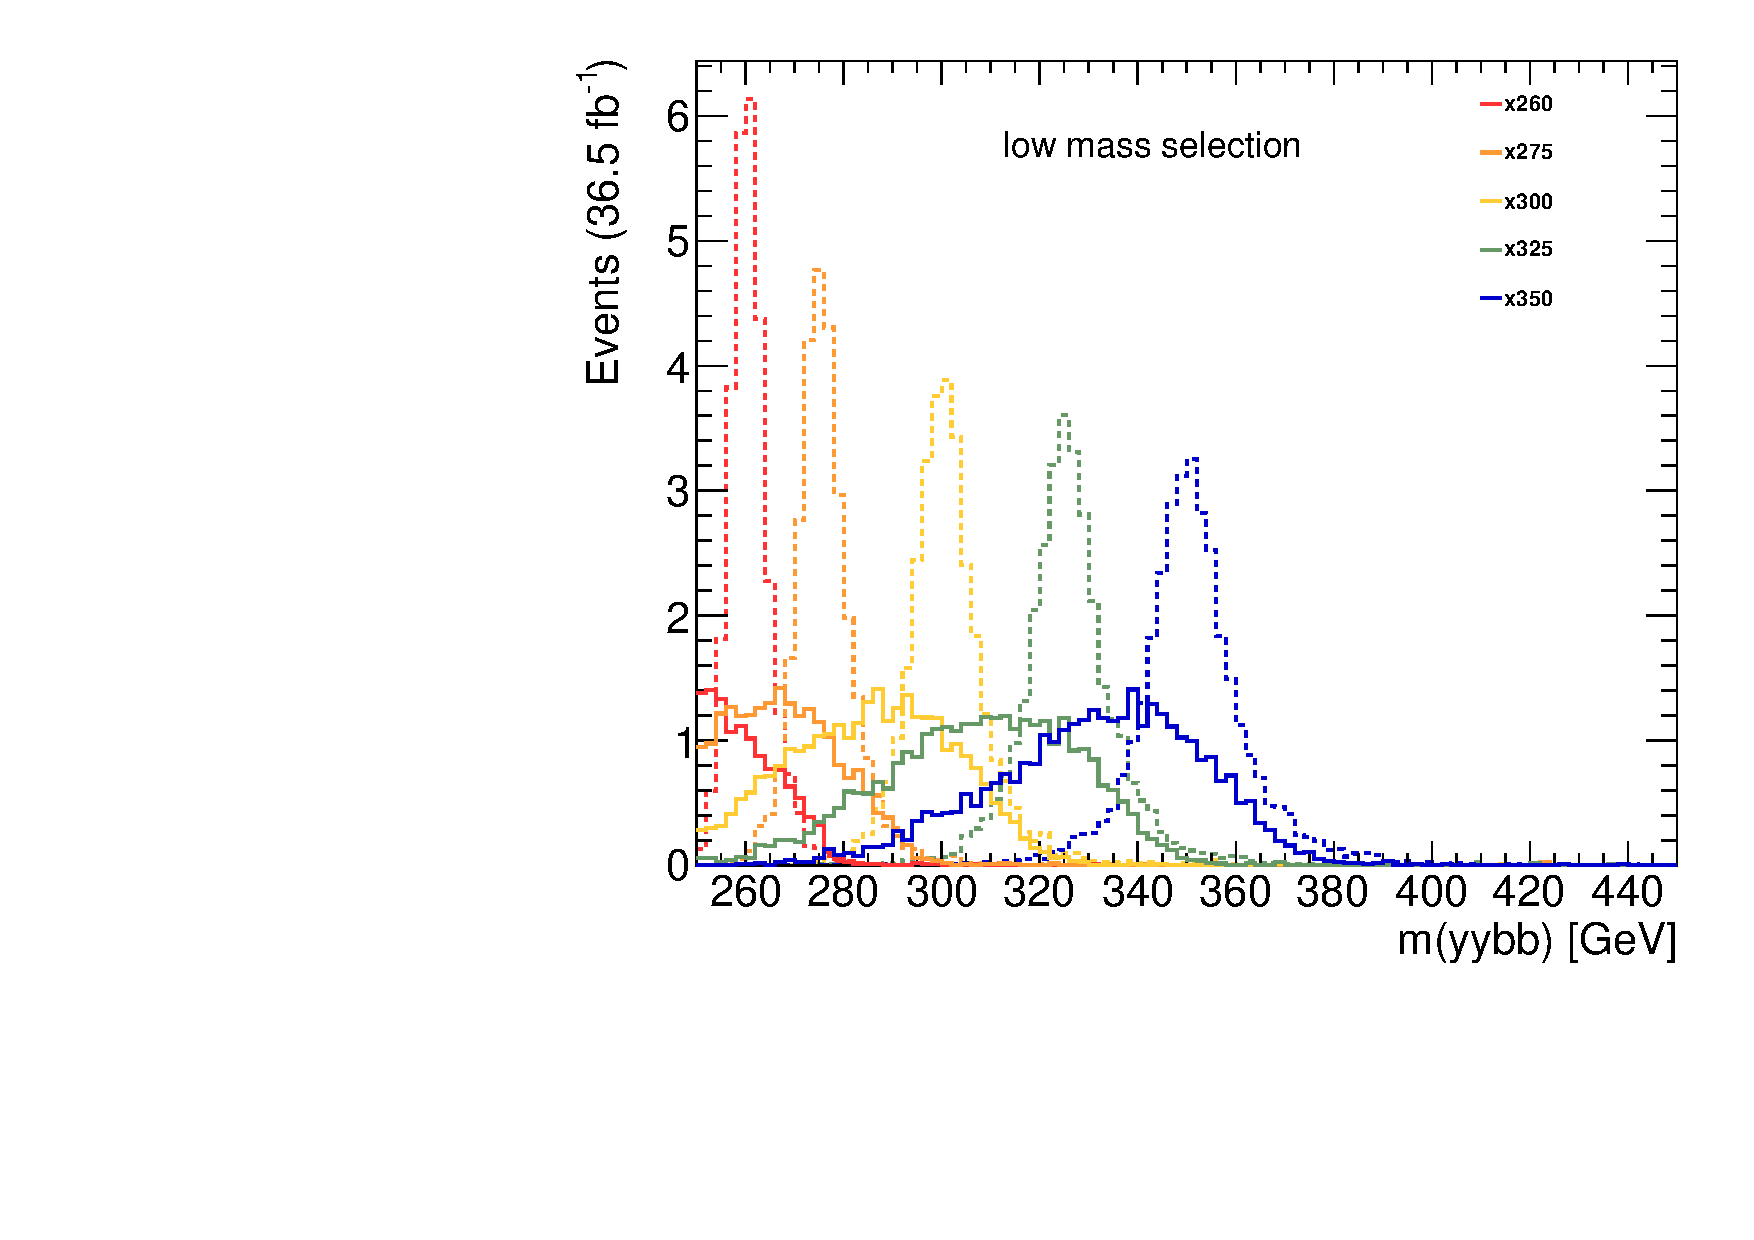
\includegraphics[width=0.48\textwidth]{chapters/chapter5_yybb/images/selection/m_yybb_low_2.pdf}}
  \subfloat[High Mass, 2-tag selection]{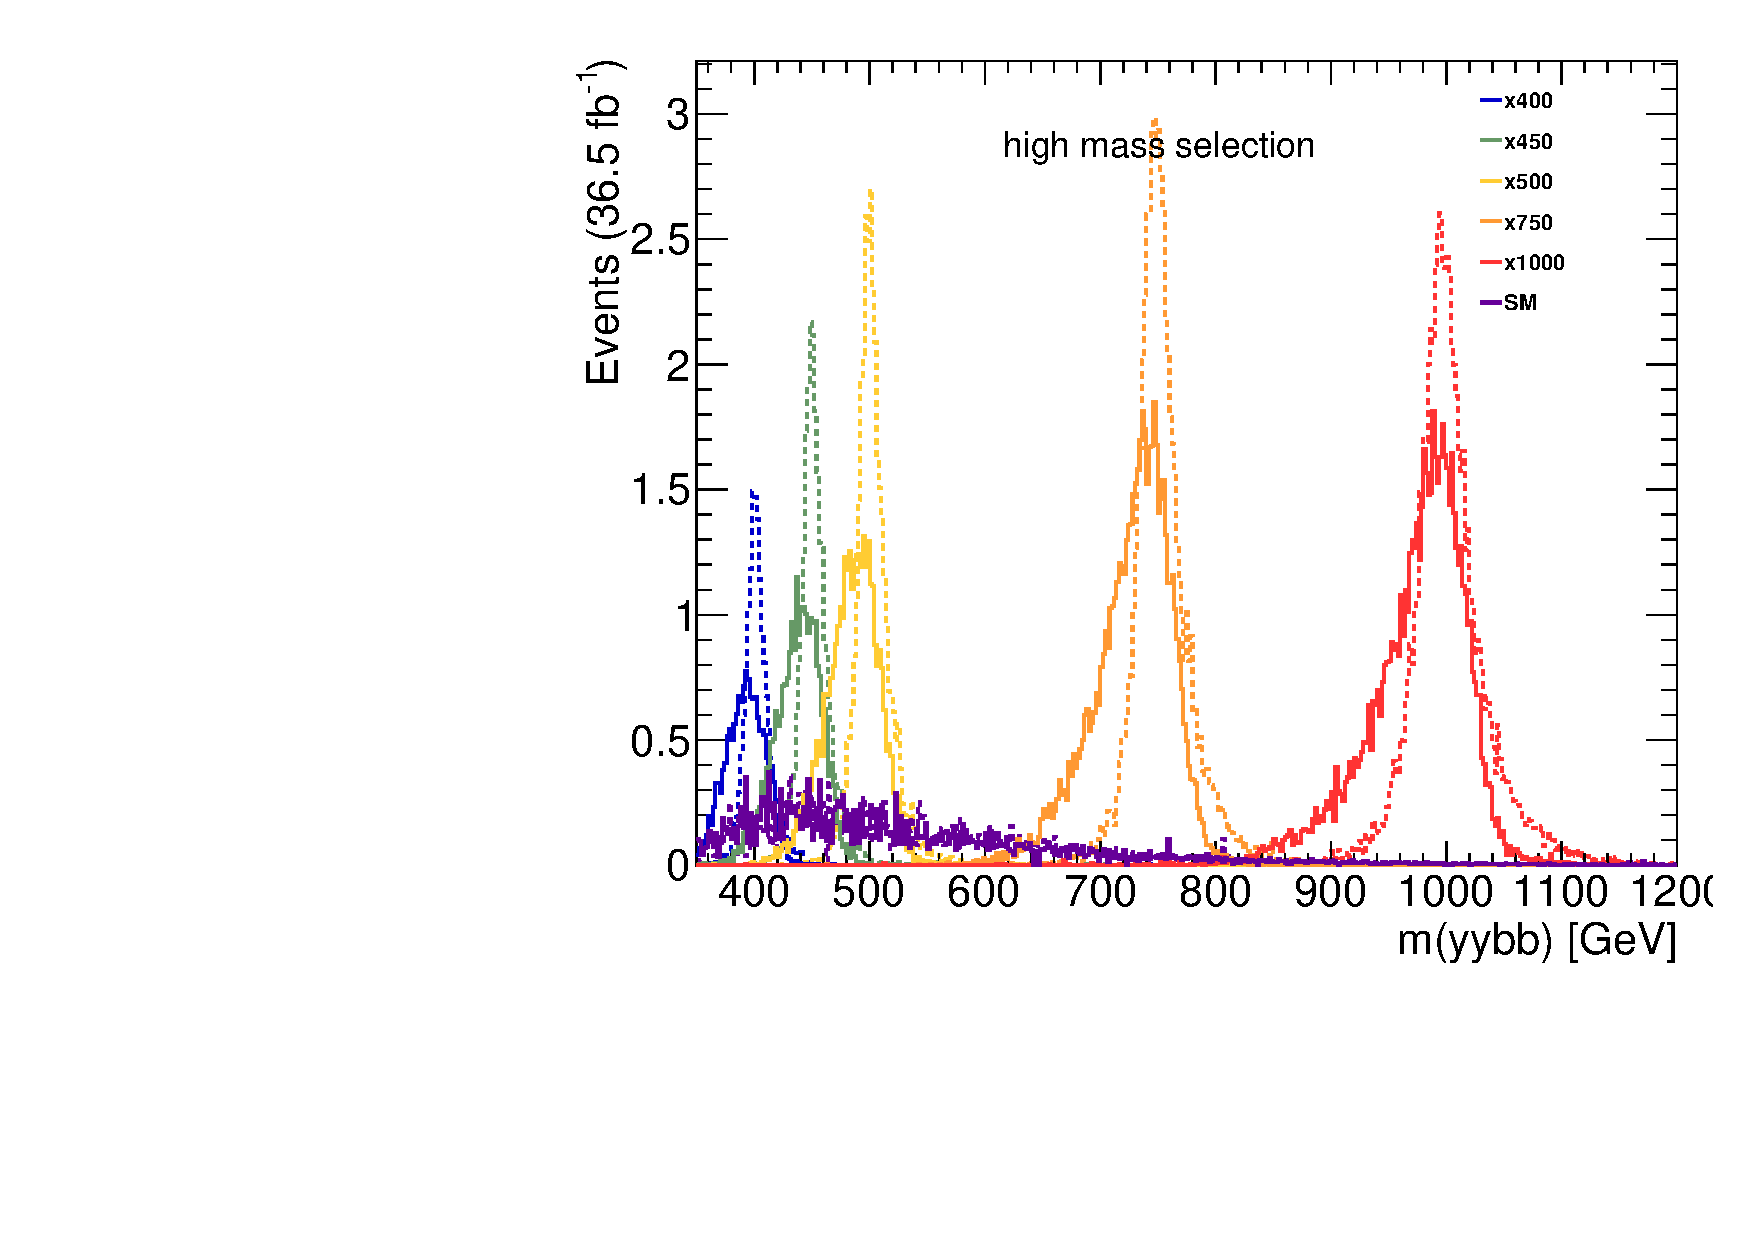
\includegraphics[width=0.48\textwidth]{chapters/chapter5_yybb/images/selection/m_yybb_high_2.pdf}}
  \caption[Reconstructed \myybb for the signal \gls{MC} samples, with and without the dijet mass constraint]
  {Reconstructed \myybb for the signal \gls{MC} samples. The solid lines show the distribution before applying the dijet mass constraint, the dashed lines have the dijet mass constraint imposed. Low and High, 1 and 2-tag selections are shown.}
  \label{fig:resolution-myybb}
\end{figure}

Last, in only the resonant analysis, a tight diphoton mass cut is applied, isolating a window around the Higgs boson mass that contains 95\% of signal events. This corresponds to $m_H \pm \unit{4.7}{\GeV}$ for the low mass selection and $m_H \pm \unit{4.3}{\GeV}$ for the high mass selection.

The absolute and relative signal efficiency for the 2 \btag region of the resonant analysis is shown in Figure \ref{fig:resonant-cutflow}. The yield and efficiency for each successive cut for the non-resonant, 2 \btag region are in Table \ref{tab:cutflow-nonres-2tag-low} and \ref{tab:cutflow-nonres-2tag-high} for the low and high mass selections, respectively. The background yield for the resonant and non-resonant selections are shown in Figure \ref{tab:background-yield}. Further cutflow studies can be found in Appendix \ref{app:cutflows}.

\begin{figure}[!h]
  \centering
  \subfloat[Low Mass Selection]{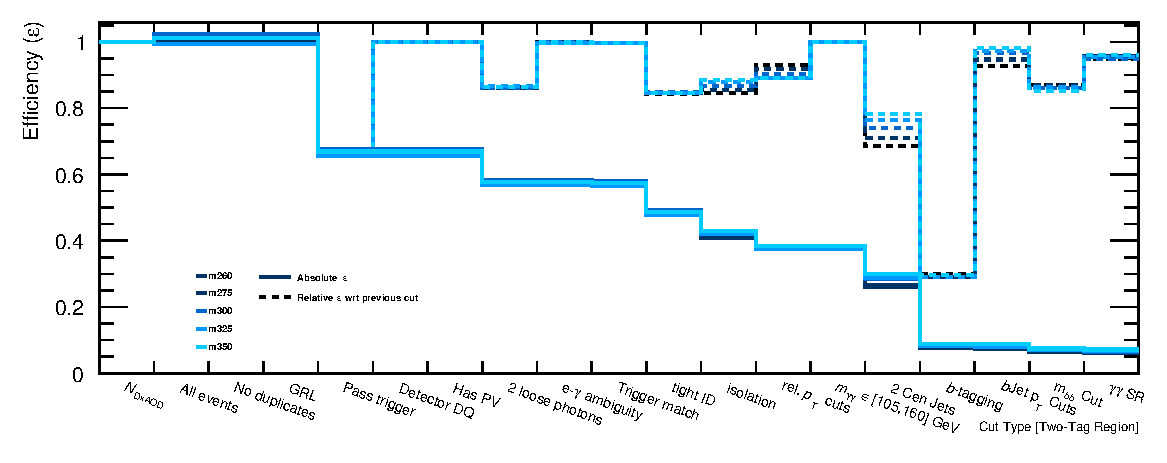
\includegraphics[width=0.9\textwidth]{chapters/chapter5_yybb/images/cutflows/TwoTag_EfficiencyOverlay_LowMass.pdf}}\\
  \subfloat[High Mass Selection]{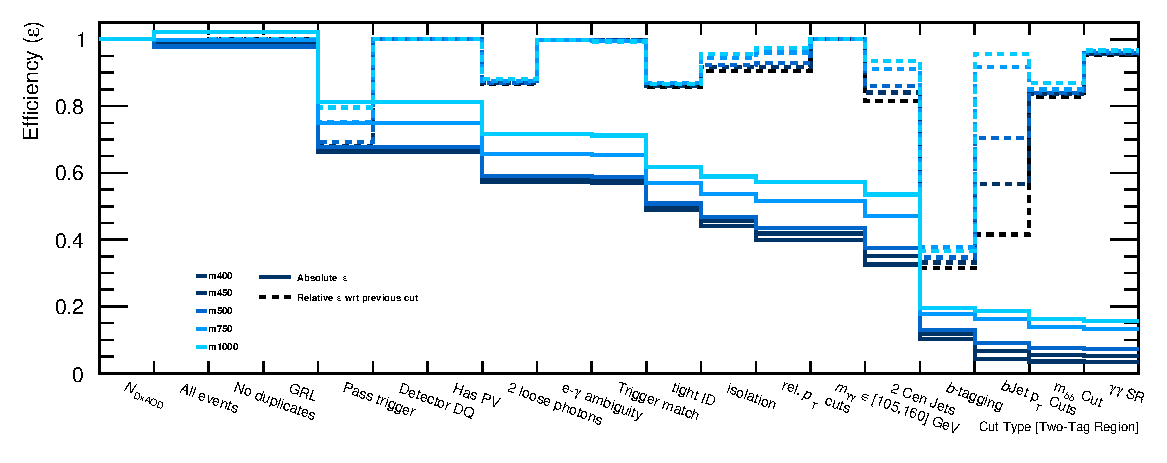
\includegraphics[width=0.9\textwidth]{chapters/chapter5_yybb/images/cutflows/TwoTag_EfficiencyOverlay_HighMass.pdf}}
  \caption[Absolute and relative efficiencies for the 2 \btag category, high mass selection]{Absolute (solid line) and relative (dotted line) efficiencies for the 2 \btag resonant signal samples to pass each cut in the low (a) and high (b) mass selection}
  \label{fig:resonant-cutflow}
\end{figure}

\begin{table}\footnotesize
\begin{center}
\caption{Cutflow for non-resonant \hhyybb - 2 tag category (low mass selection)}
\label{tab:cutflow-nonres-2tag-low}
\begin{tabular}{|c|c|c|c|}
 \hline
Cuts& \multicolumn{3}{c|}{2 b-tag} \\ \hline
 &Yield&Error&Efficiency\\ \hline
$N_{xAOD}$ & 3.147&0.027 &$-$ \\
 \hline
$\it{N}_{DxAOD}$ & 3.147&0.019 &$-$ \\
 \hline
$All\ events$ & 3.181&0.024 &100.0 \\
 \hline
$No\ duplicates$ & 3.181&0.024 &100.0 \\
 \hline
$GRL$ & 3.181&0.024 &100.0 \\
 \hline
$Pass\ trigger$ & 2.184&0.021 &68.7 \\
 \hline
$Detector\ DQ$ & 2.184&0.021 &68.7 \\
 \hline
$Has\ PV$ & 2.184&0.021 &68.7 \\
 \hline
$2\ loose\ photons$ & 1.894&0.019 &59.5 \\
 \hline
$e-\gamma\ ambiguity$ & 1.891&0.019 &59.5 \\
 \hline
$Trigger\ match$ & 1.885&0.019 &59.3 \\
 \hline
$tight\ ID$ & 1.617&0.018 &50.8 \\
 \hline
$isolation$ & 1.476&0.017 &46.4 \\
 \hline
$rel.\ p_{T}\ cuts$ & 1.362&0.017 &42.8 \\
 \hline
$m_{\gamma\gamma}\ \in\ [105,160]\ GeV$ & 1.362&0.017 &42.8 \\
 \hline
$2\ Cen\ Jets$ & 1.149&0.016 &36.1 \\
 \hline
$b-tagging$ & 0.373&0.008 &11.7 \\
 \hline
$bJet\ p_{T}\ Cuts$ & 0.369&0.008 &11.6 \\
 \hline
$m_{bb}\ Cut$ & 0.318&0.007 &10.0 \\
 \hline
$\gamma\gamma\ SR$ & 0.305&0.007 & 9.6 \\
 \hline
\end{tabular}
\end{center}
\end{table}

\begin{table}\footnotesize
\begin{center}
\caption{Cutflow for non-resonant \hhyybb, 2 tag category (high mass selection). A description of the cuts is listed in the caption of Table \ref{tab:cutflow-nonres-2tag-low}.}
\label{tab:cutflow-nonres-2tag-high}
\begin{tabular}{|c|c|c|c|}
 \hline
Cuts& \multicolumn{3}{c|}{2 b-tag} \\ \hline
 &Yield&Error&Efficiency\\ \hline
$N_{xAOD}$ & 3.147&0.027 &$-$ \\
 \hline
$\it{N}_{DxAOD}$ & 3.147&0.019 &$-$ \\
 \hline
$All\ events$ & 3.181&0.024 &100.0 \\
 \hline
$No\ duplicates$ & 3.181&0.024 &100.0 \\
 \hline
$GRL$ & 3.181&0.024 &100.0 \\
 \hline
$Pass\ trigger$ & 2.184&0.021 &68.7 \\
 \hline
$Detector\ DQ$ & 2.184&0.021 &68.7 \\
 \hline
$Has\ PV$ & 2.184&0.021 &68.7 \\
 \hline
$2\ loose\ photons$ & 1.894&0.019 &59.5 \\
 \hline
$e-\gamma\ ambiguity$ & 1.891&0.019 &59.5 \\
 \hline
$Trigger\ match$ & 1.885&0.019 &59.3 \\
 \hline
$tight\ ID$ & 1.617&0.018 &50.8 \\
 \hline
$isolation$ & 1.476&0.017 &46.4 \\
 \hline
$rel.\ p_{T}\ cuts$ & 1.362&0.017 &42.8 \\
 \hline
$m_{\gamma\gamma}\ \in\ [105,160]\ GeV$ & 1.362&0.017 &42.8 \\
 \hline
$2\ Cen\ Jets$ & 1.149&0.016 &36.1 \\
 \hline
$b-tagging$ & 0.373&0.008 &11.7 \\
 \hline
$bJet\ p_{T}\ Cuts$ & 0.219&0.005 & 6.9 \\
 \hline
$m_{bb}\ Cut$ & 0.183&0.005 & 5.8 \\
 \hline
$\gamma\gamma\ SR$ & 0.175&0.005 & 5.5 \\
 \hline
\end{tabular}
\end{center}
\end{table}


\begin{table}[h] %TODO: find error on the yy continuum
  \caption[Background yield in the 2 \btag region split by process for the non-resonant and resonant analyses]{Background yield in the 2 \btag region split by process for the non-resonant and resonant analyses. The non-resonant analysis requires passing of all cuts but the \myy SR constraint, and is denoted by the ``Yield'' column. The resonant analysis includes the additional \myy constraint and is denoted ``SR Yield.''}
  \label{tab:background-yield}
  \begin{tabular}{|l|llll|llll|}
  \hline
  2-tag Category & \multicolumn{4}{c|}{Low Mass}     & \multicolumn{4}{c|}{High Mass}    \\ \hline
  Background     &  Yield  & Error & SR Yield & Error & Yield  & Error & SR Yield & Error \\ 
  \yy-continuum   & 109.79 &       & 21.03    &       & 23.58  &       & 4.03     &     \\ 
  $ggH$            & 0.315  & 0.035 & 0.306    & 0.035 & 0.074  & 0.013 & 0.073    & 0.013 \\ 
  VBF $H$           & 0.042  & 0.004 & 0.041    & 0.004 & 0.007  & 0.002 & 0.006    & 0.002 \\ 
  $W^-H$            & 0.004  & 0.001 & 0.004    & 0.001 & 0.002  & 0.001 & 0.001    & 0.001 \\ 
  $W^+H$            & 0.007  & 0.002 & 0.006    & 0.002 & 0.002  & 0.001 & 0.002    & 0.001 \\ 
  $ZH$             & 0.388  & 0.009 & 0.378    & 0.009 & 0.095  & 0.005 & 0.094    & 0.005 \\ 
  $ggZH$           & 0.129  & 0.007 & 0.128    & 0.007 & 0.048  & 0.004 & 0.048    & 0.004 \\ 
  $ttH$            & 1.363  & 0.015 & 1.331    & 0.015 & 0.353  & 0.008 & 0.343    & 0.008 \\ 
  $bbH$ (positive)   & 0.016  & 0.024 & 0.014    & 0.023 & -0.005 & 0.005 & -0.005   & 0.005 \\ 
  $bbH$ (negative)   & -0.004 & 0.001 & -0.005   & 0.001 & 0.000  & 0.000 & 0.000    & 0.000 \\ \hline
  \end{tabular}
  \end{table}

\section{Modeling}

In both the resonant and non-resonant analyses, a full signal+background fit is performed. For the non-resonant analysis, the \myy spectrum is fit, while for the resonant analysis the \myybb is fit. This section describes the parameterization to model the signal and background of each analysis.

\subsection{Background Composition} \label{ssec:background-composition}

The \yy-continuum background contains contributions from both diphoton events, as well as those where jets fake photons, denoted $j\gamma$, $\gamma j$, or $jj$, where the leading, subleading, or both photons have been misidentified jets, respectively. To establish the contributions of each of these sources, a 2x2D sideband method \cite{2x2d-sideband} is used. This method varies the photon identification and isolation criteria to create a signal region and 15 control regions, then expresses the yield, identification efficiency, and isolation efficiency for both photons and jets in each region. Using this, along with the correlations between isolation distributions, a global minimization procedure is used to calculate the \yy, $j\gamma$, $\gamma j$, and $jj$ yield separately for the 1 and 2 b-tag categories. In all cases, the \yy contribution is dominant, representing 80-90\% of events. This method is described in detail in Appendix \ref{app:2x2d}. The relative contributions are shown in Figure \ref{fig:background_fractions}.


\begin{figure}[b!]
  \centering
  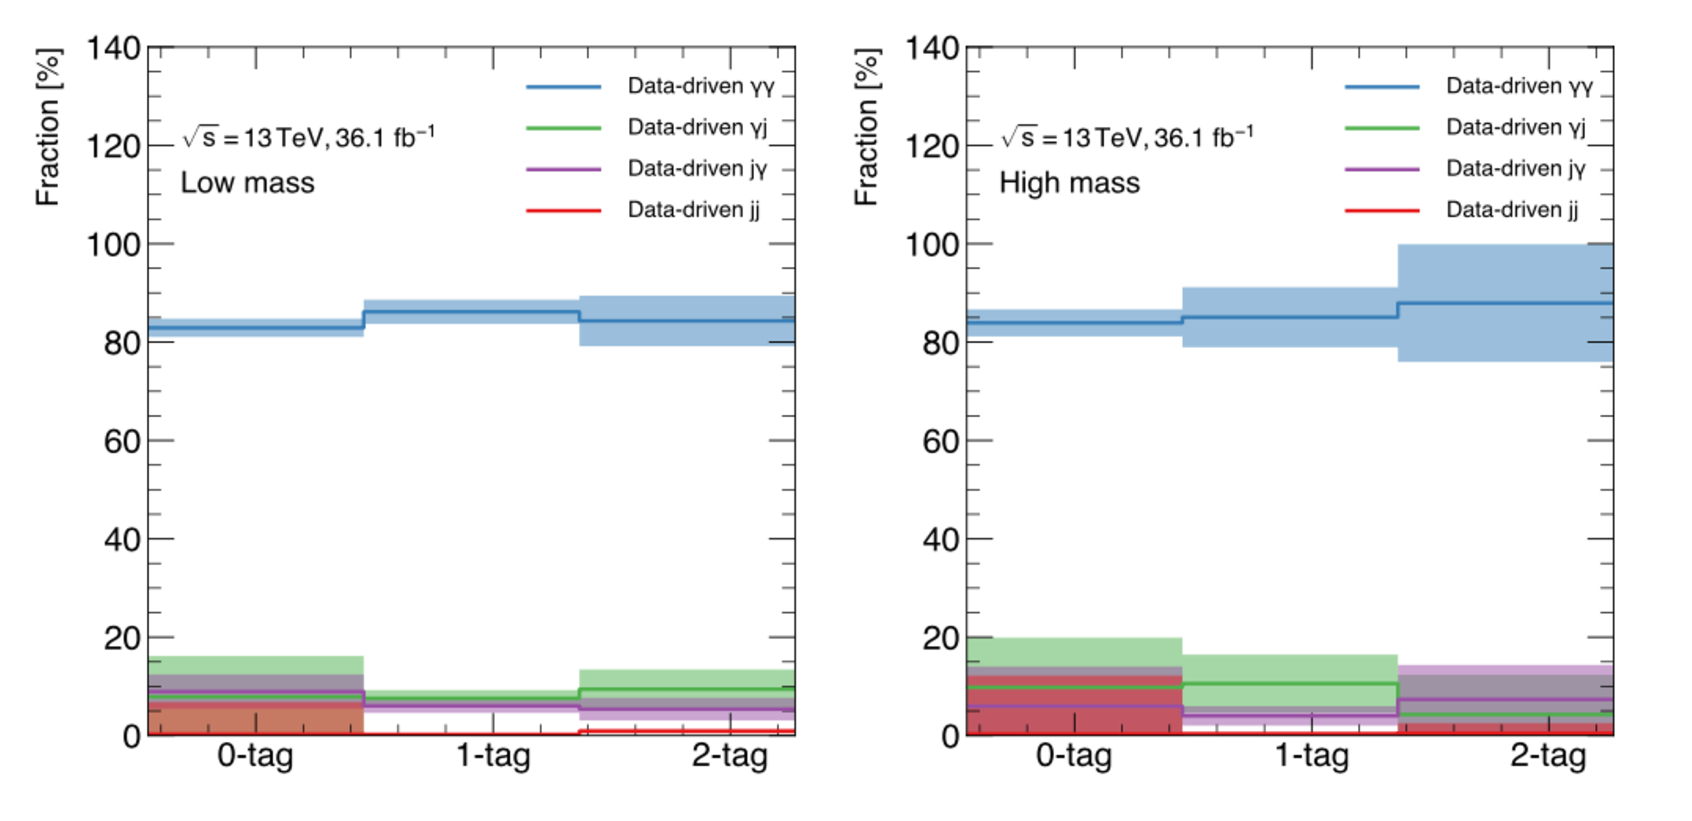
\includegraphics[width=\textwidth]{chapters/chapter5_yybb/images/2x2d/expected_contribution_clean.pdf}
  \caption{Expected contributions from \yy, \yj, \jy and \jj to the 2015+2016 data for the low mass (left) and high mass (right) selections.
    \label{fig:background_fractions}}
\end{figure}


In order to get expected shapes of the \yy, \yj, \jy and \jj contributions, the 2x2D method is applied bin-wise in \myy (bins defined in width of 2.5 GeV between 105 and 160 GeV). First, a template for each category is produced using the high stats \yy-continuum sample. For the \yy contribution, this requires both photons passing both tight identification and FixedCutLoose isolation. For the \yj, \jy and \jj, this requires photons which pass loose requirements, but do not fall into the \yy category.

These templates from \gls{MC} are then compared to the data-driven 2x2D method and reweighted to better match data. The template and 2x2D templates are separately fitted using an exponential of second order polynomial function and their ratio is used as a smooth reweighting function in \myy. Figures \ref{fig:2x2D_templates_lowMass} and \ref{fig:2x2D_templates_highMass} show this for the low and high mass selection respectively, in the 0-tag region. There are insufficient statistics to perform this in the 1 and 2 \btag regions, however the same reweighting functions from the 0-tag may be applied. For the final continuum \yy background prediction, the proportions shown in Figure \ref{fig:background_fractions} are used. The fractional contribution is shown in Table \ref{tab:modelling-background-fractions}. The normalization is chosen such that the sideband region ($105 < \myy < 120$ GeV and $130 < \myy <160$ GeV) contribution is equal to the contribution in data.

\begin{figure}[!hp]
  \centering
  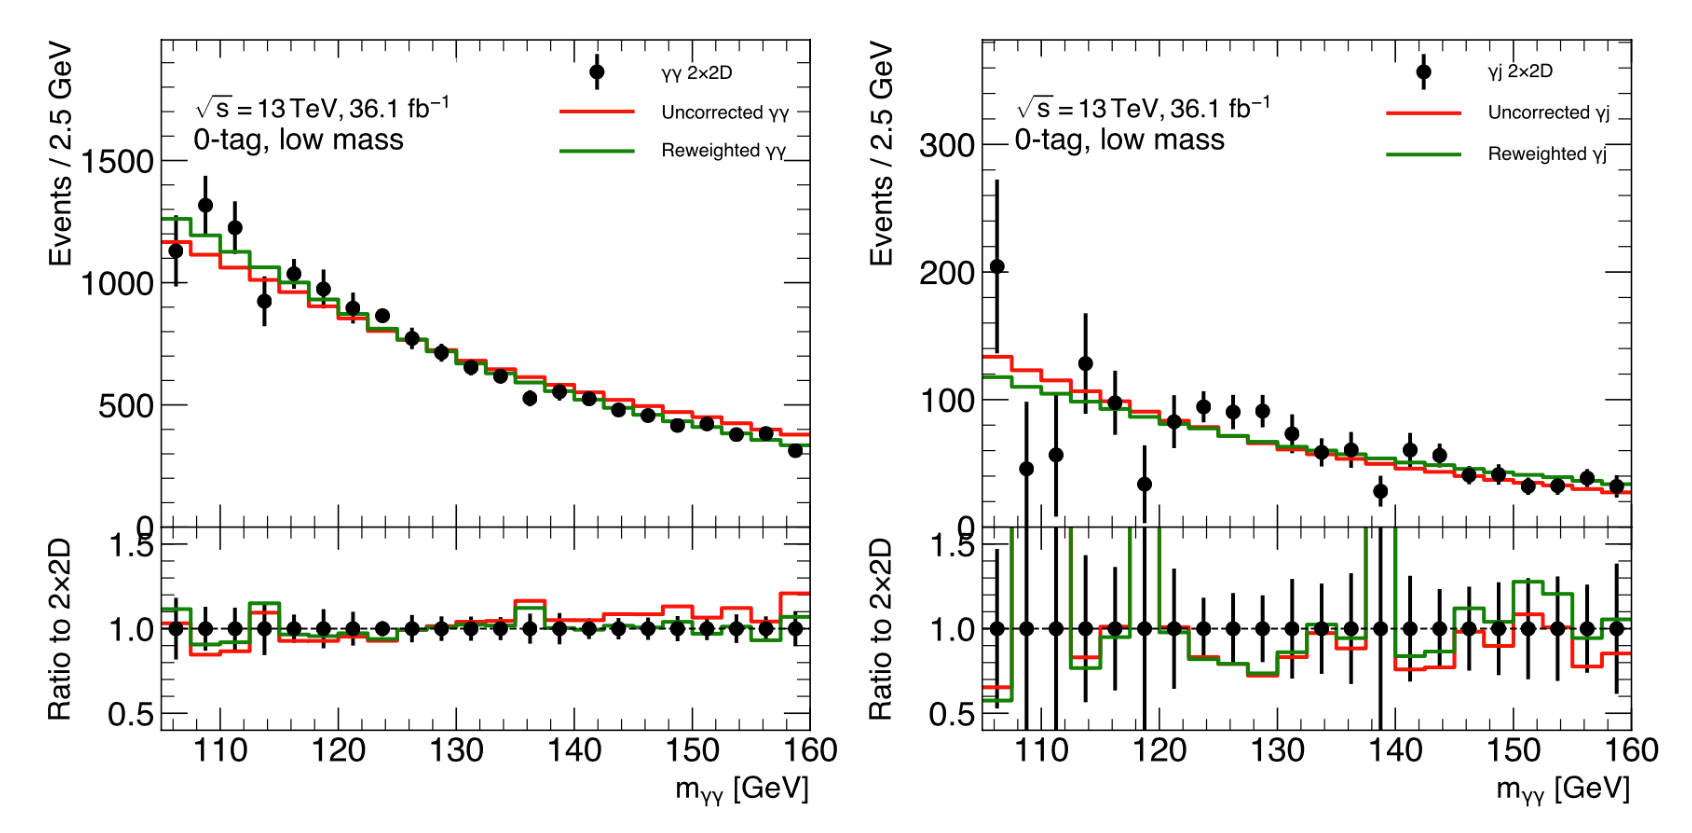
\includegraphics[width=\textwidth]{chapters/chapter5_yybb/images/2x2d/low_mass_1_clean.pdf}\\
  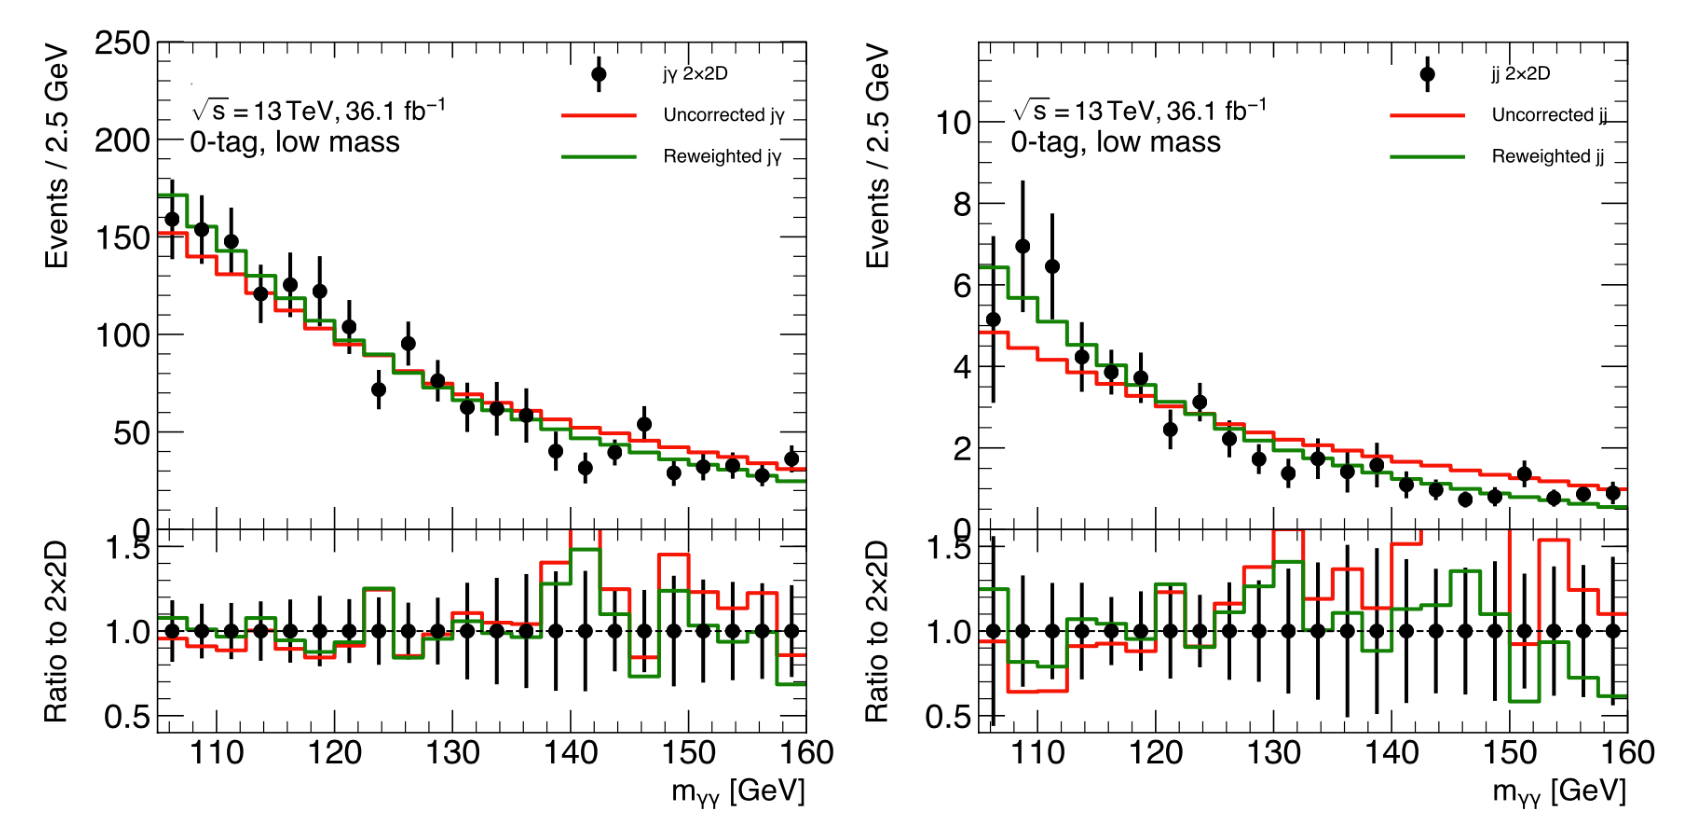
\includegraphics[width=\textwidth]{chapters/chapter5_yybb/images/2x2d/low_mass_2_clean.pdf}
  \caption{Template distributions for each of the \yy, \yj, \jy and \jj  components from Sherpa (red) and after reweighting (green) are compared to the output of the 2x2D method for 0-tag events with the low mass selection.
    \label{fig:2x2D_templates_lowMass}}
\end{figure}

\begin{figure}[!hp]
  \centering
  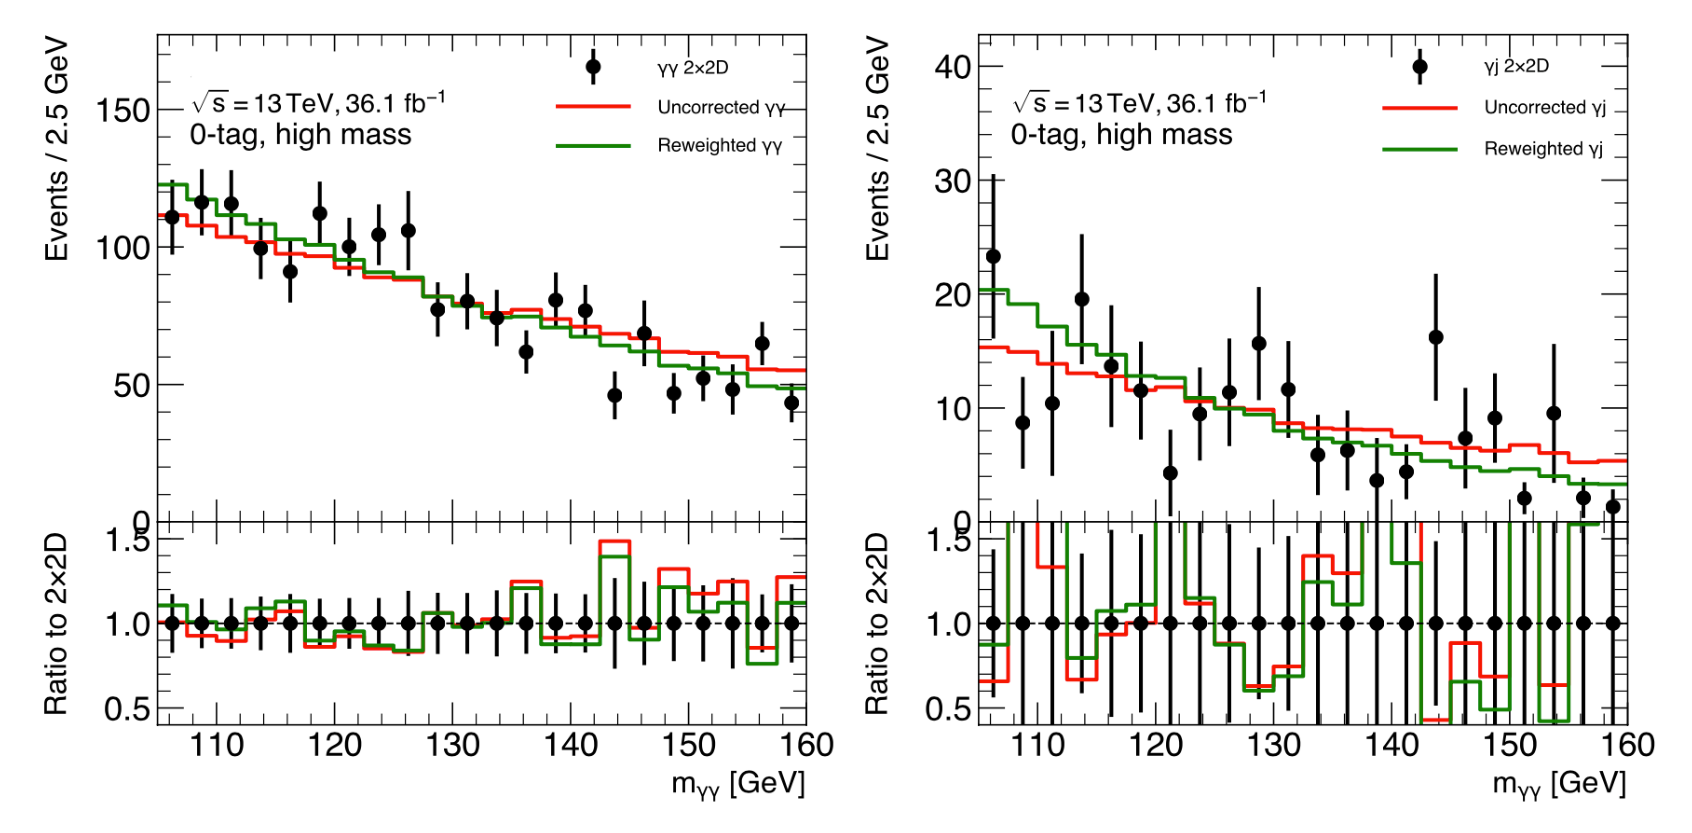
\includegraphics[width=\textwidth]{chapters/chapter5_yybb/images/2x2d/high_mass_1_clean.pdf}\\
  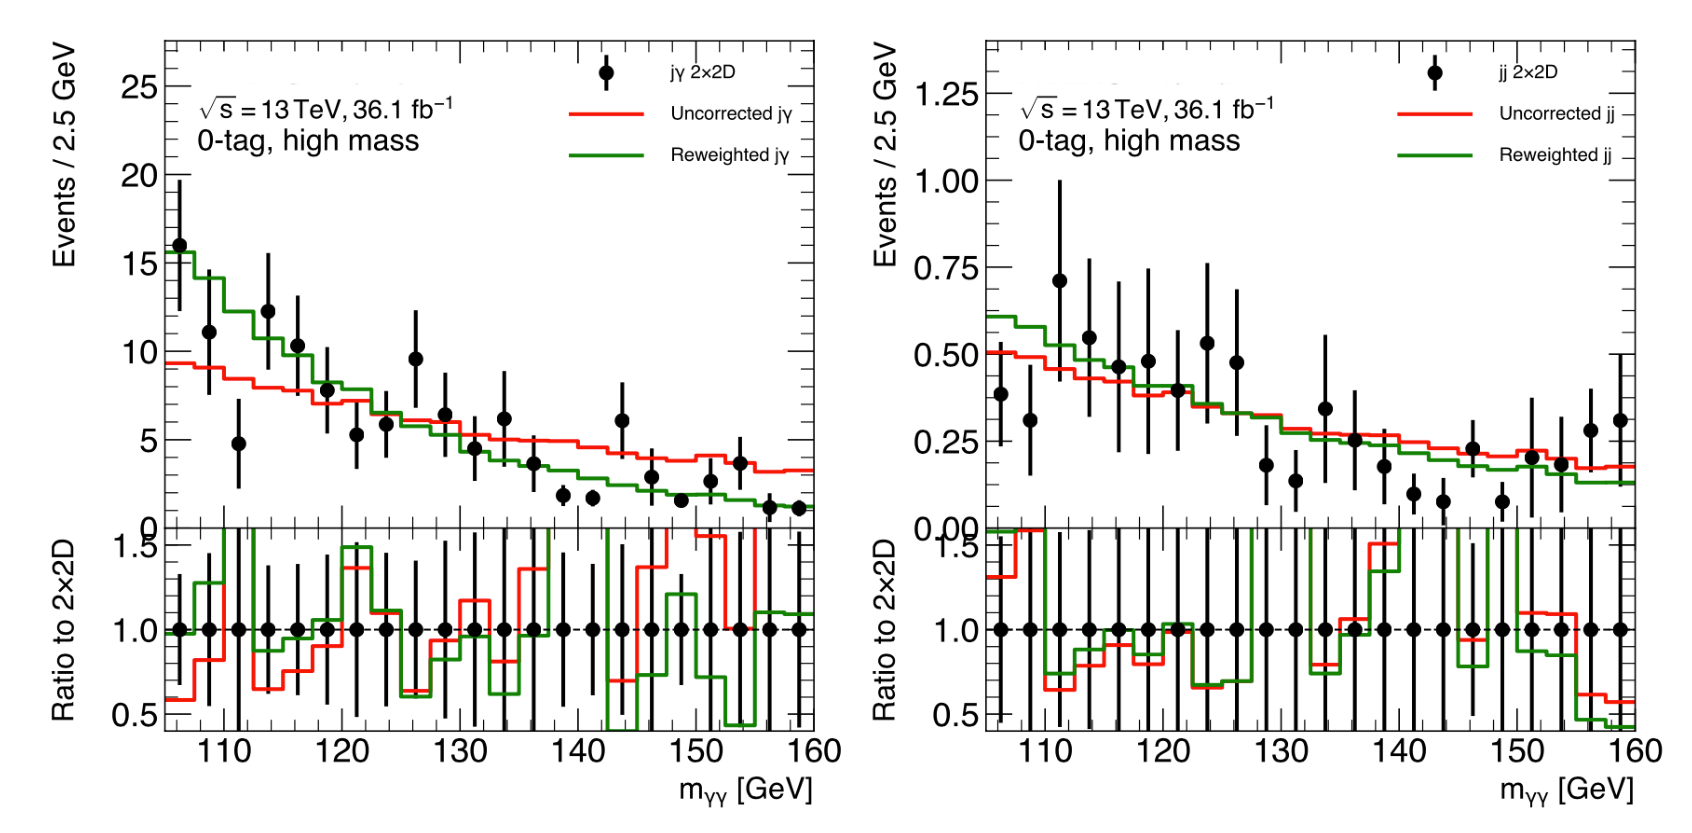
\includegraphics[width=\textwidth]{chapters/chapter5_yybb/images/2x2d/high_mass_2_clean.pdf}
  \caption{Template distributions for each of the \yy, \yj, \jy and \jj components from Sherpa (red) and after reweighting (green) are compared to the output of the 2x2D method for 0-tag events with the high mass selection.
    \label{fig:2x2D_templates_highMass}}
\end{figure}

\begin{table}[!h]
  \caption{Expected fractional contributions from \yy, \yj, \jy and \jj to the events passing the nominal selection in each of the 0-, 1- and 2-tag categories.}
  \label{tab:modelling-background-fractions}
  \begin{center}
    \begin{tabular}{c c c c c c c}
      \toprule
            & \multicolumn{2}{c}{0-Tag}         & \multicolumn{2}{c}{1-Tag}         & \multicolumn{2}{c}{2-Tag}         \\
            & Low mass        & High mass       & Low mass        & High mass       & Low mass        & High mass       \\
        \midrule
        \yy & $0.99 \pm 0.08$ & $0.85 \pm 0.01$ & $0.85 \pm 0.02$ & $0.84 \pm 0.09$ & $0.85 \pm 0.05$ & $0.68 \pm 0.22$ \\
        \yj & $0.00 \pm 0.04$ & $0.07 \pm 0.01$ & $0.07 \pm 0.02$ & $0.07 \pm 0.07$ & $0.08 \pm 0.04$ & $0.09 \pm 0.14$ \\
        \jy & $0.00 \pm 0.03$ & $0.07 \pm 0.01$ & $0.07 \pm 0.02$ & $0.08 \pm 0.04$ & $0.06 \pm 0.03$ & $0.18 \pm 0.13$ \\
        \jj & $0.00 \pm 0.00$ & $0.01 \pm 0.00$ & $0.01 \pm 0.00$ & $0.01 \pm 0.01$ & $0.02 \pm 0.01$ & $0.05 \pm 0.06$ \\
        \bottomrule
    \end{tabular}
\end{center}
\end{table}





\subsection{Modeling in the Non-resonant Analysis}
\subsubsection{Signal Modeling}

A double-sided Crystal Ball function \cite{dscb-diphoton}, a Gaussian core with power-law tails, is used to describe the shape of the \hhyybb signal. Model parameters are taken from the simulated signal sample. Figure \ref{fig:SMhh_DoubleCB} shows the parameterization using the high mass selection, and Figure \ref{fig:SMhh_DoubleCB_low} shows the parameterization with the low mass selection.

%% TOdo rewrite these captions
\begin{figure}[p!]
  \centering
  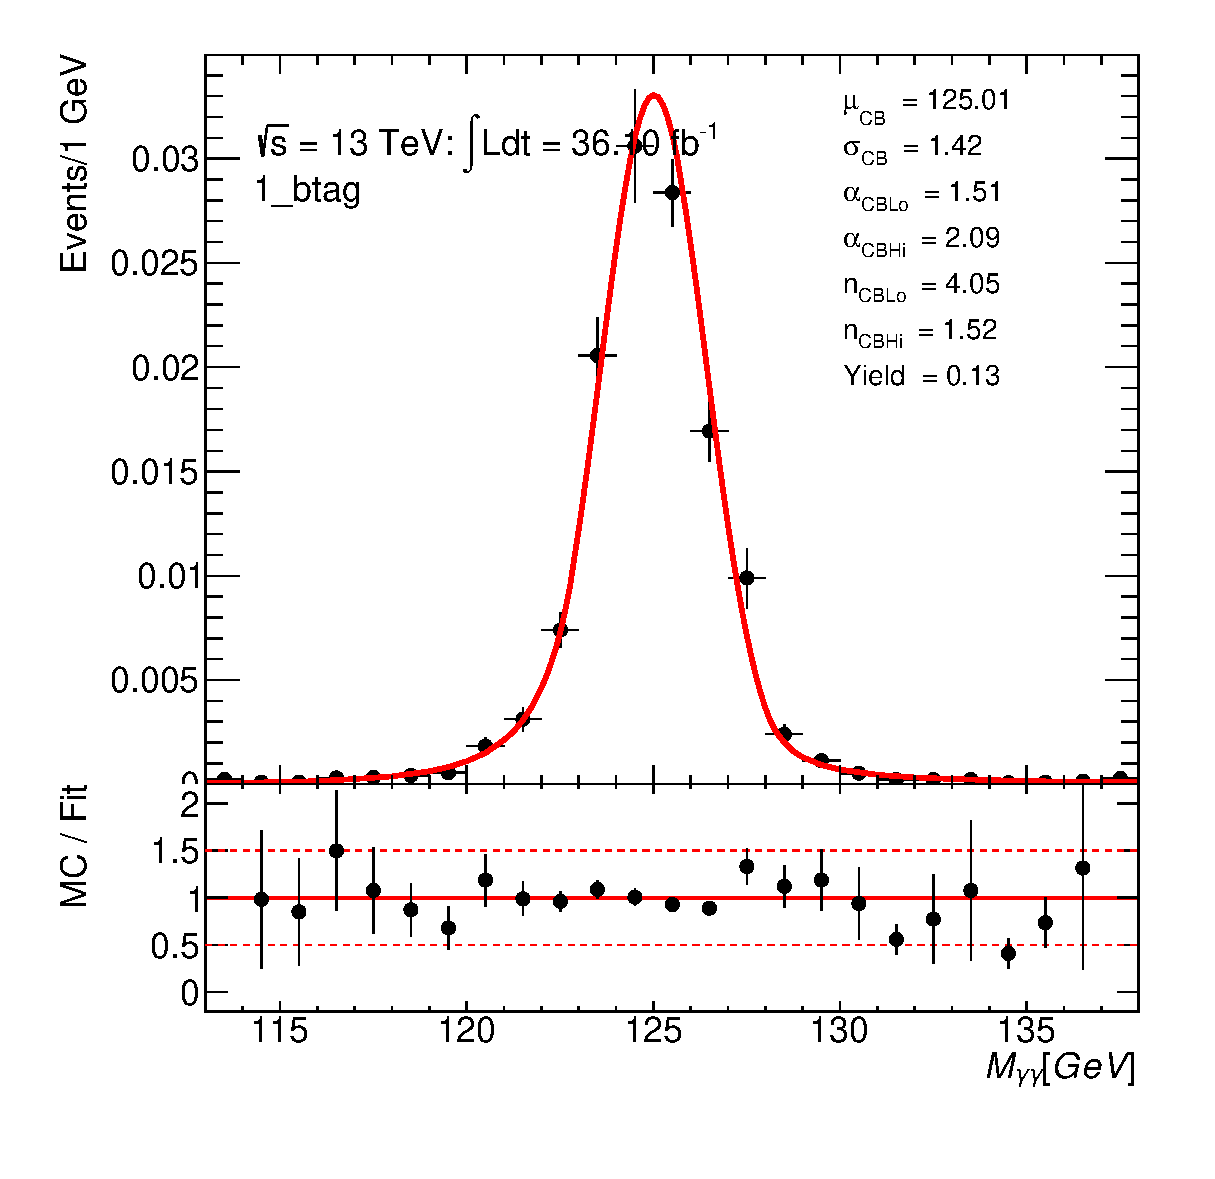
\includegraphics[width=0.48\textwidth]{{chapters/chapter5_yybb/images/parameterization/plot_singleRes_m125.00_c1_afterfix_nlo}.eps}
  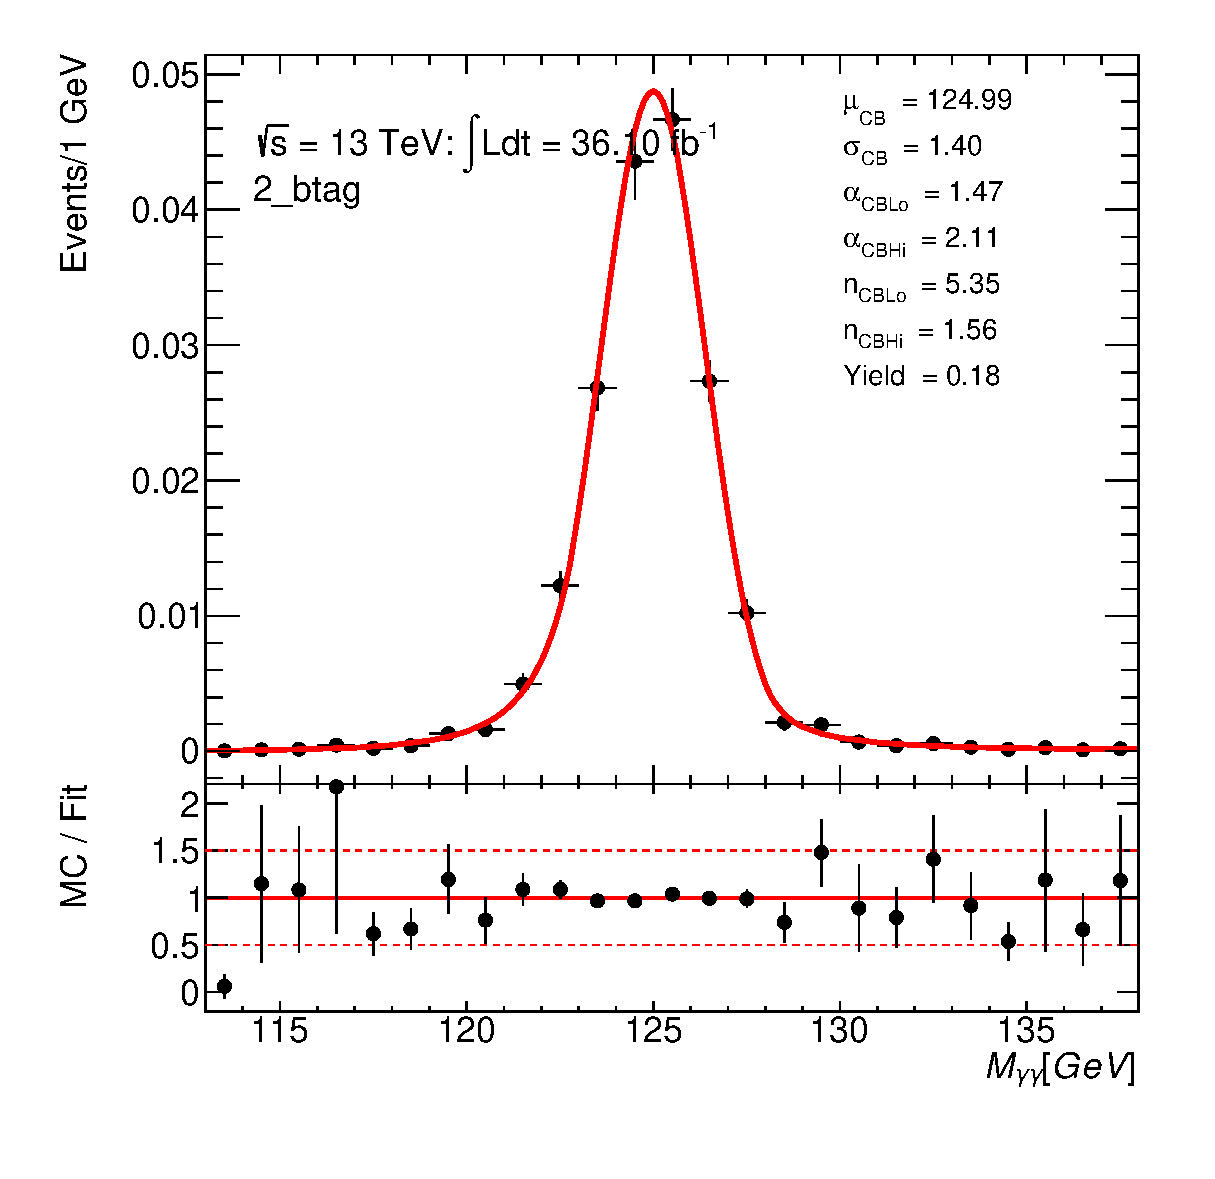
\includegraphics[width=0.48\textwidth]{{chapters/chapter5_yybb/images/parameterization/plot_singleRes_m125.00_c2_afterfix_nlo}.eps}
  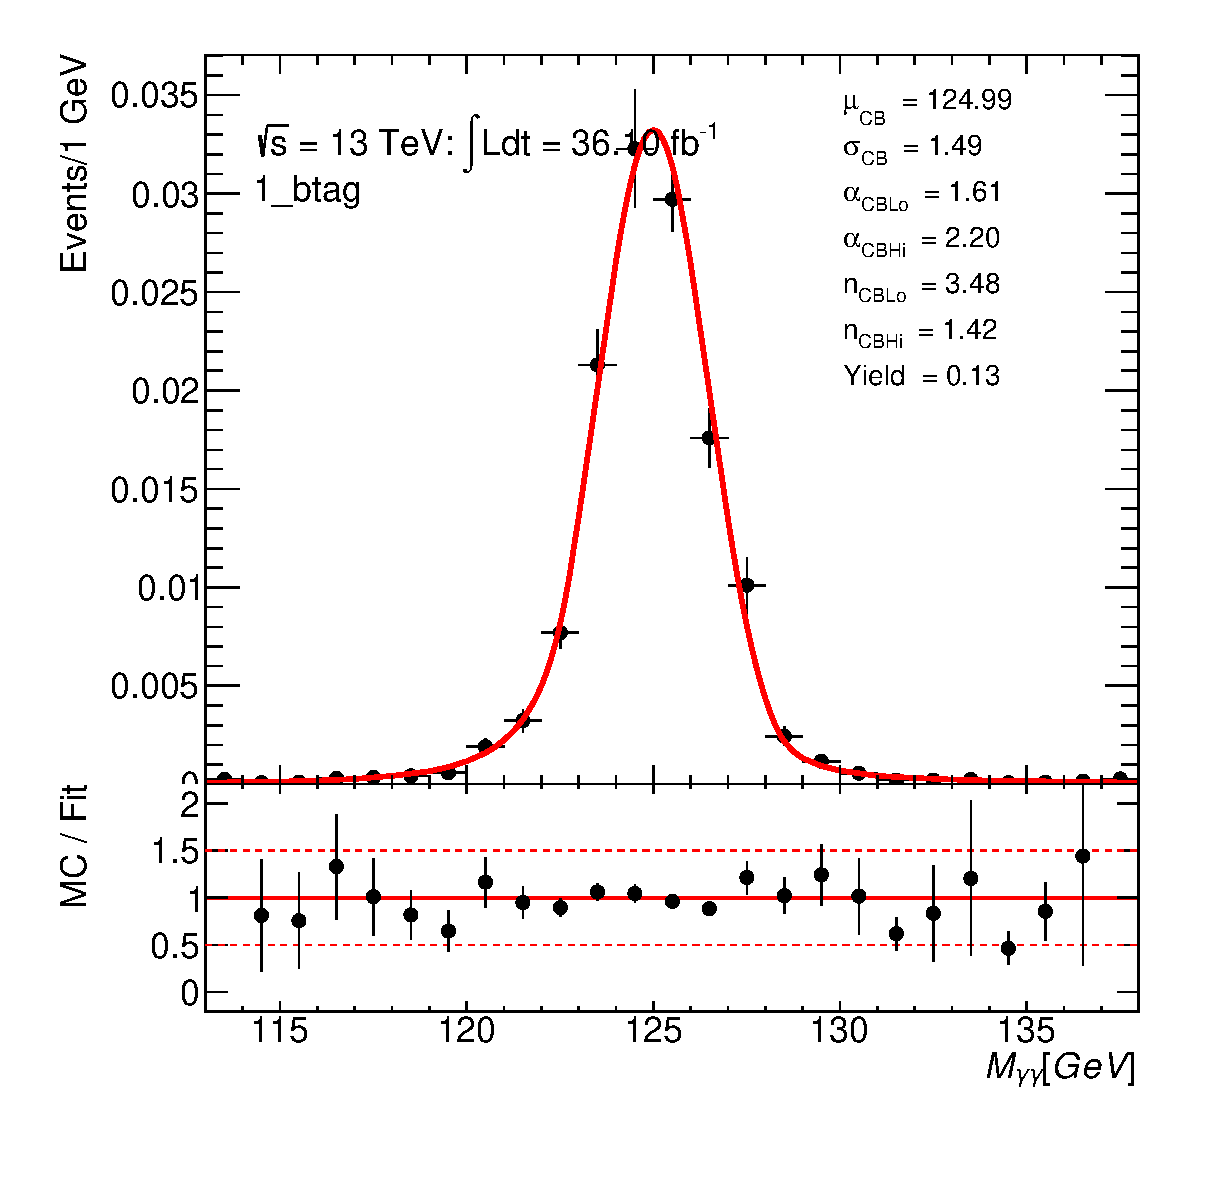
\includegraphics[width=0.48\textwidth]{{chapters/chapter5_yybb/images/parameterization/plot_singleRes_m125.00_c1_afterfix_lo}.eps}
  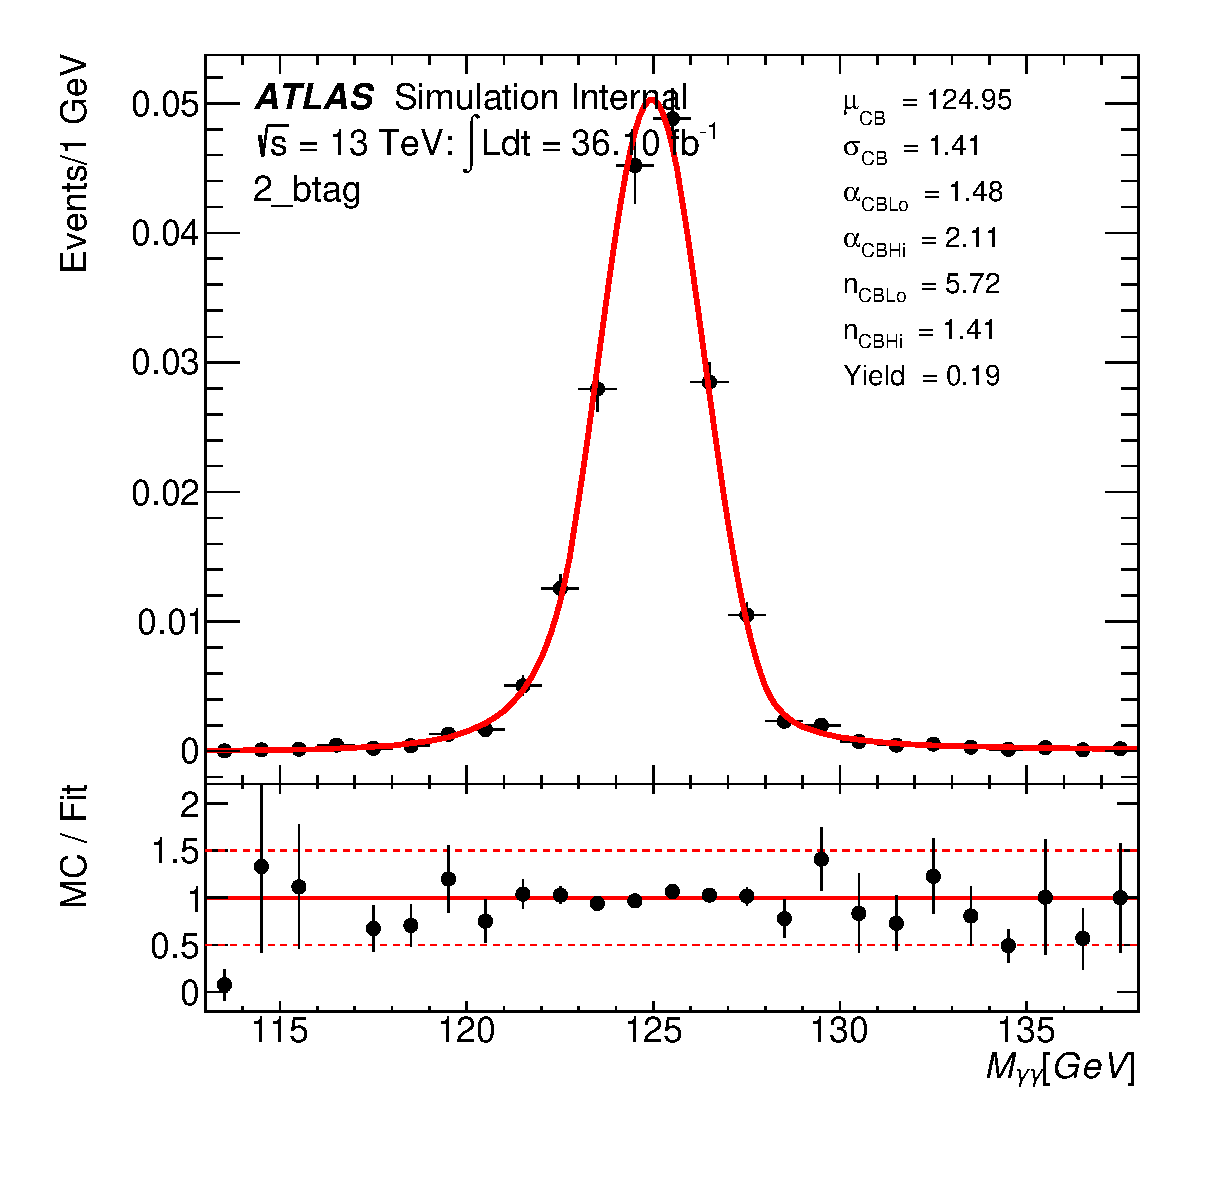
\includegraphics[width=0.48\textwidth]{{chapters/chapter5_yybb/images/parameterization/plot_singleRes_m125.00_c2_afterfix_lo}.eps}
  \caption[SM di-Higgs diphoton parameterization with a double-sided Crystal Ball function]{Parameterization of the $\myy$ distribution from the SM di-Higgs simulated samples at a mass of 125 GeV in the 1-tag (left) and 2-tag (right) categories, with (top) and without the signal MC reweighting to full NLO (bottom). Events were required to pass the high mass selection.
  \label{fig:SMhh_DoubleCB}}
\end{figure}

\begin{figure}[p!]
	\centering
	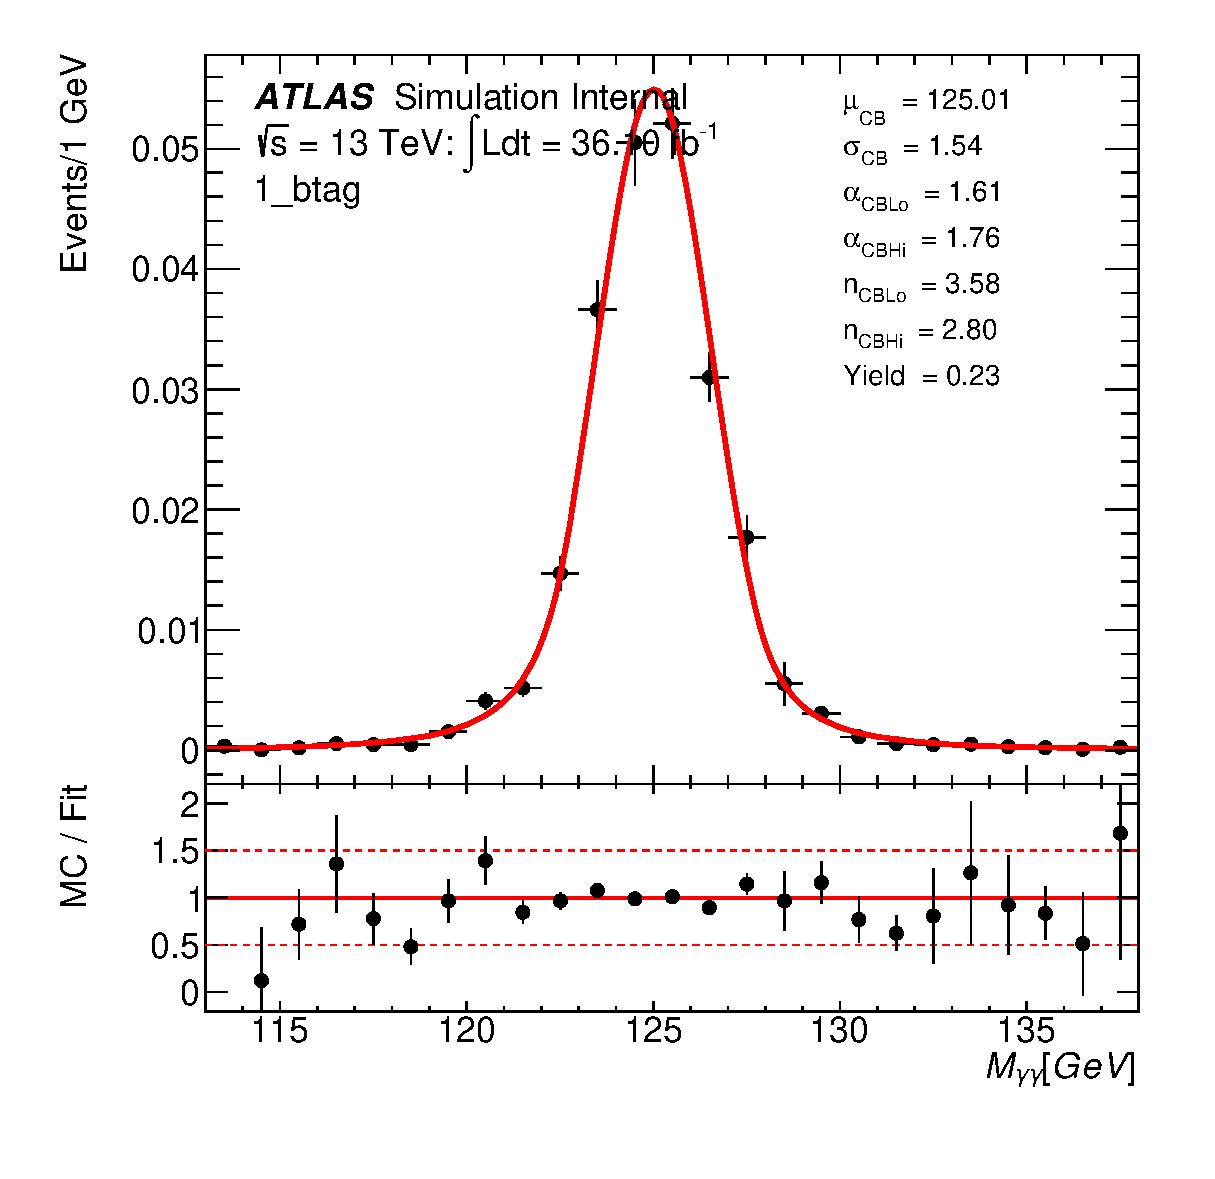
\includegraphics[width=0.48\textwidth]{{chapters/chapter5_yybb/images/parameterization/plot_singleRes_m125.00_c1_afterfix_low_nlo}.eps}
	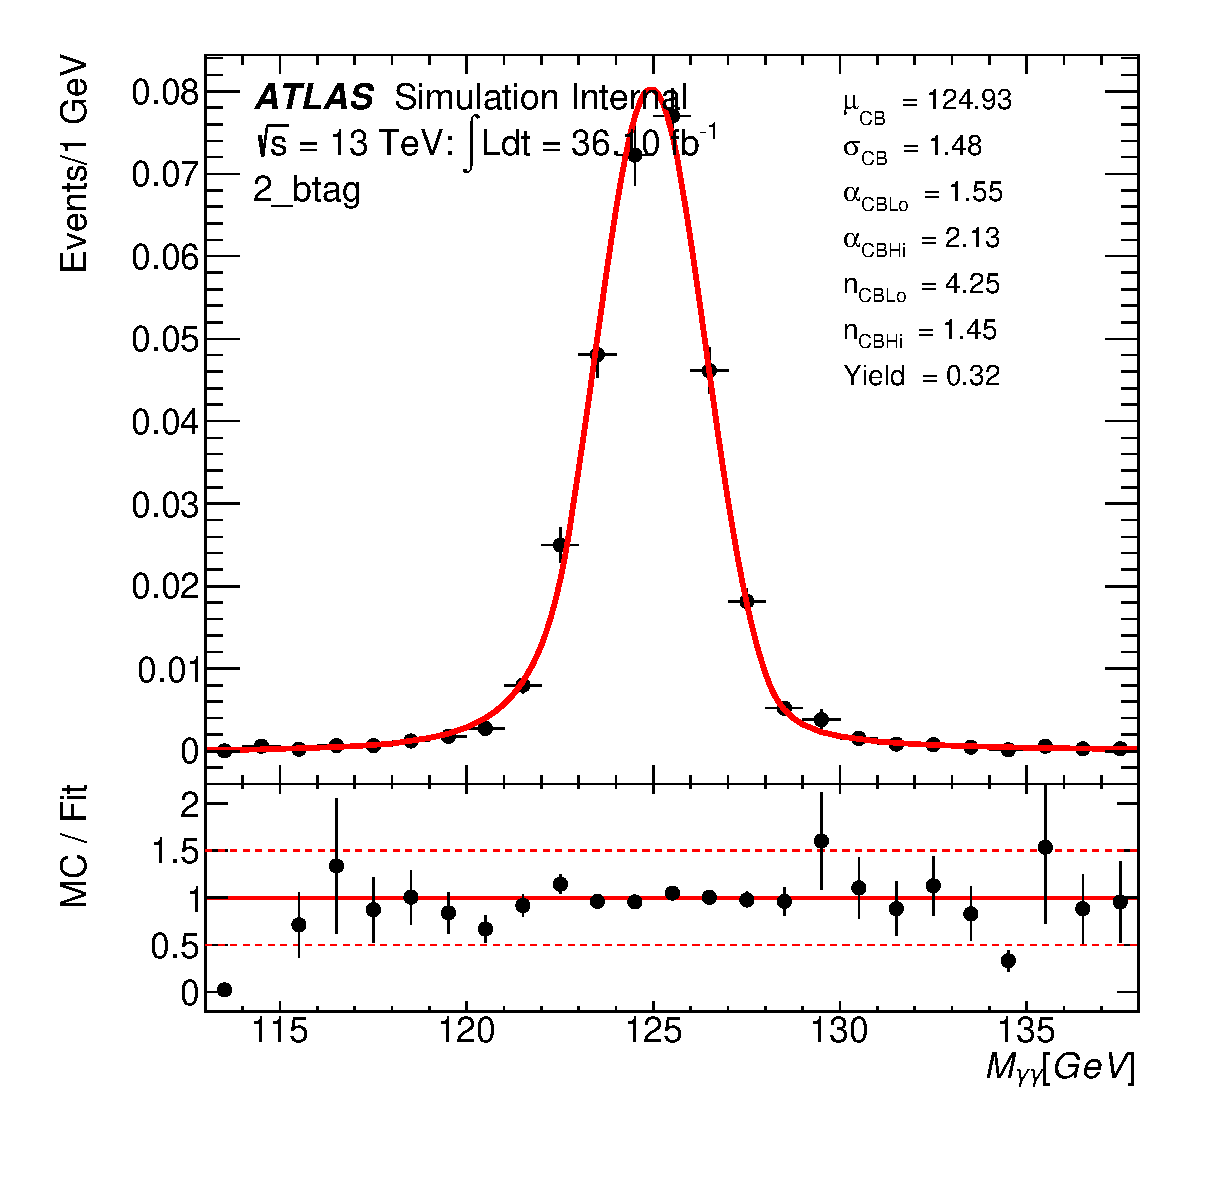
\includegraphics[width=0.48\textwidth]{{chapters/chapter5_yybb/images/parameterization/plot_singleRes_m125.00_c2_afterfix_low_nlo}.eps}
	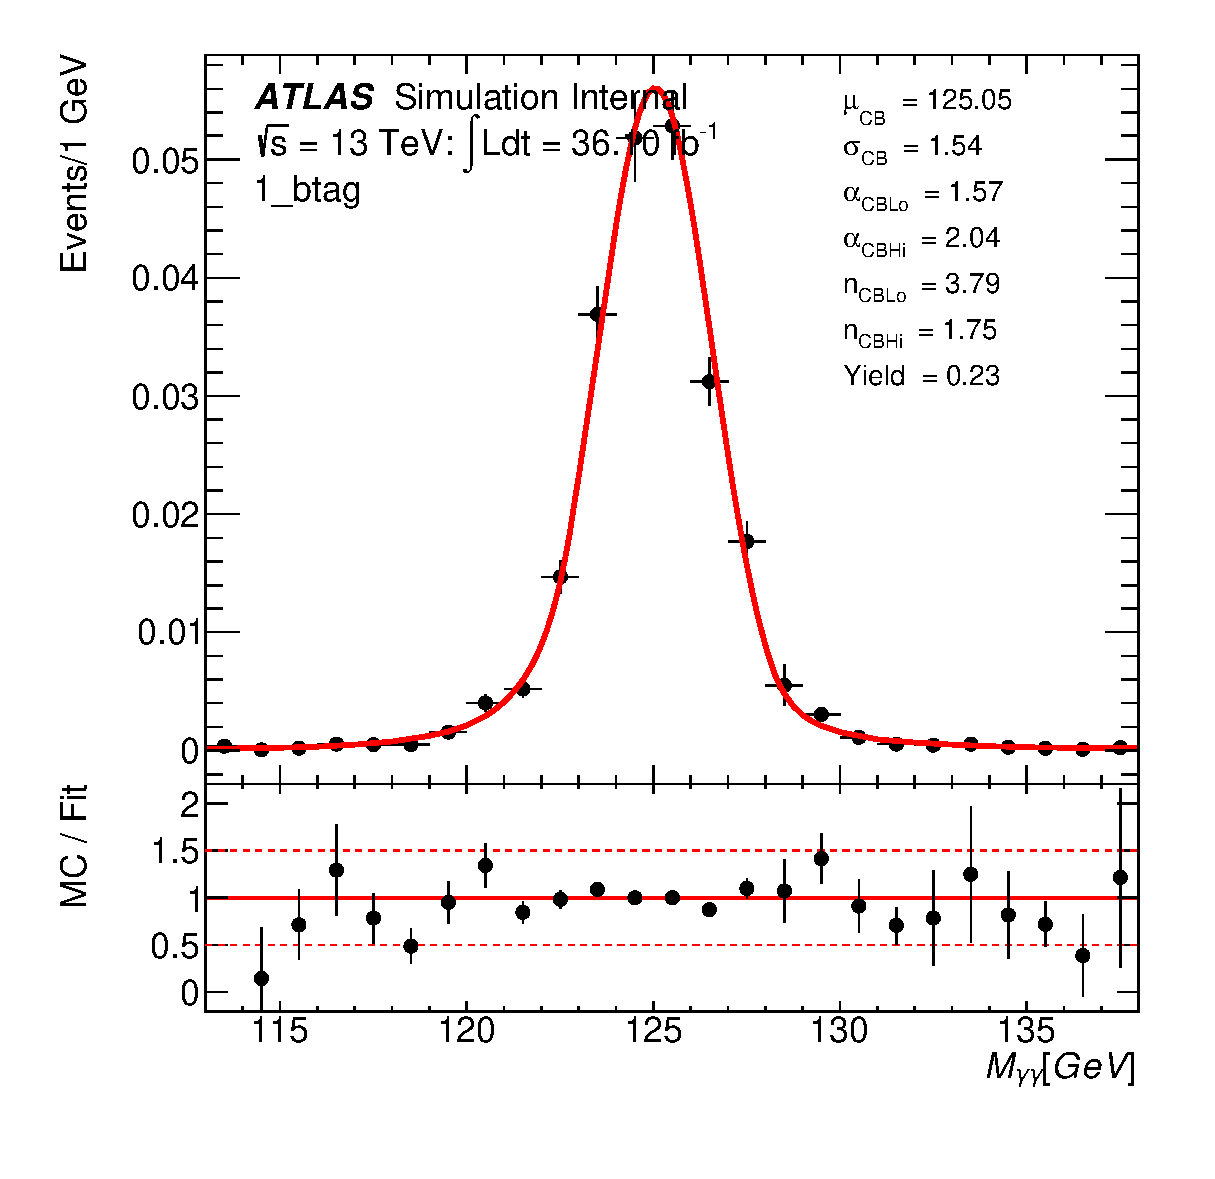
\includegraphics[width=0.48\textwidth]{{chapters/chapter5_yybb/images/parameterization/plot_singleRes_m125.00_c1_afterfix_low_lo}.eps}
	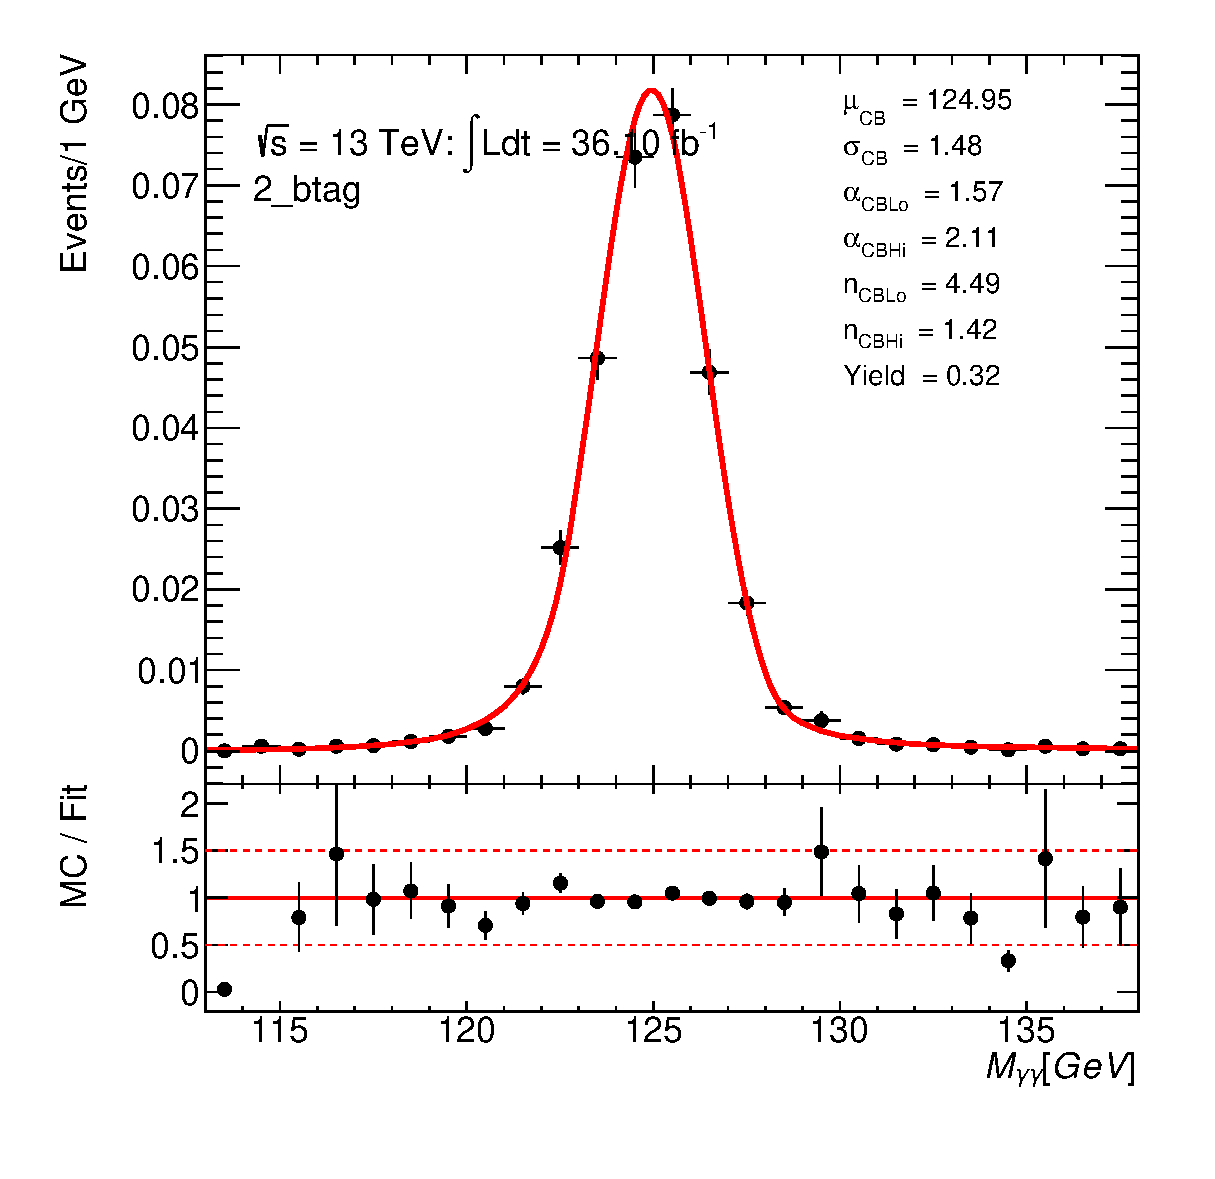
\includegraphics[width=0.48\textwidth]{{chapters/chapter5_yybb/images/parameterization/plot_singleRes_m125.00_c2_afterfix_low_lo}.eps}
	\caption[SM di-Higgs diphoton parameterization with a double-sided Crystal Ball function]{Parameterization of the $\myy$ distribution from the SM di-Higgs simulated samples at a mass of 125 GeV in the 1-tag (left) and 2-tag (right) categories, with (top) and without the signal MC reweighting to full NLO (bottom). Events were required to pass the low mass selection.
	\label{fig:SMhh_DoubleCB_low}}
\end{figure}


\subsubsection{Background Modeling} \label{sssec:nonres-bkg-model}

The background for the non-resonant analysis is composed of a model for the smoothly-falling \yy-continuum, and a model for single Higgs boson production. 


For the \yy-continuum background, a functional form is fit to data. The fit function is selected through a \textit{spurious signal} test \cite{spurious-signal-diphoton}, which evaluates potential bias from this procedure. This test performs signal-plus-background fits to just the simulated background, evaluating the extracted signal in the $\unit{121}{\GeV} < \myy < \unit{129}{\GeV}$ window, which is taken as the bias. This procedure is repeated for each considered function, and the function with the fewest spurious signal events is selected as the background function. If functions have the same bias, then by an Occam's Razor argument, the function with fewer free parameters is selected. The considered functions for this test are as follows:
\begin{itemize}
  \item Exponential, consider orders $N=1,2,3$. Generalized form: $Exp^N (\myy ; \theta^{bkg}) = exp(\sum\limits_{j=0}^{N} \theta_j^{bkg} \dot m_{\gamma\gamma}^j)$
  \item Bernstein, consider orders $N=3,4,5$. Generalized form: $Bernstein^N (\myy ; \theta^{bkg}) = \sum\limits_{j=0}^{N} \theta_j^{bkg} b_{j,N}$, for $b_{j,N} = C_n^i x^j (1-x)^{N-j}$, where $x= (\myy-100)/60$
  \item Dijet of form: $dijet(\myy ; \theta^{bkg}) = \theta_1^{bkg} (1-\myy)^{\theta_2^{bkg}} m_{\gamma\gamma}^{\theta_3^{bkg}}$
\end{itemize}

Through this test, the first-order exponential function is found to have the lowest bias, and is selected as the \yy-continuum background model. This fit is shown for both selections in the 1 and 2-tag categories in Figure \ref{fig:bkg-fit-myy}.

\begin{figure}[b!]
  \centering
  \subfloat[Low mass selection, 1 b-tag]{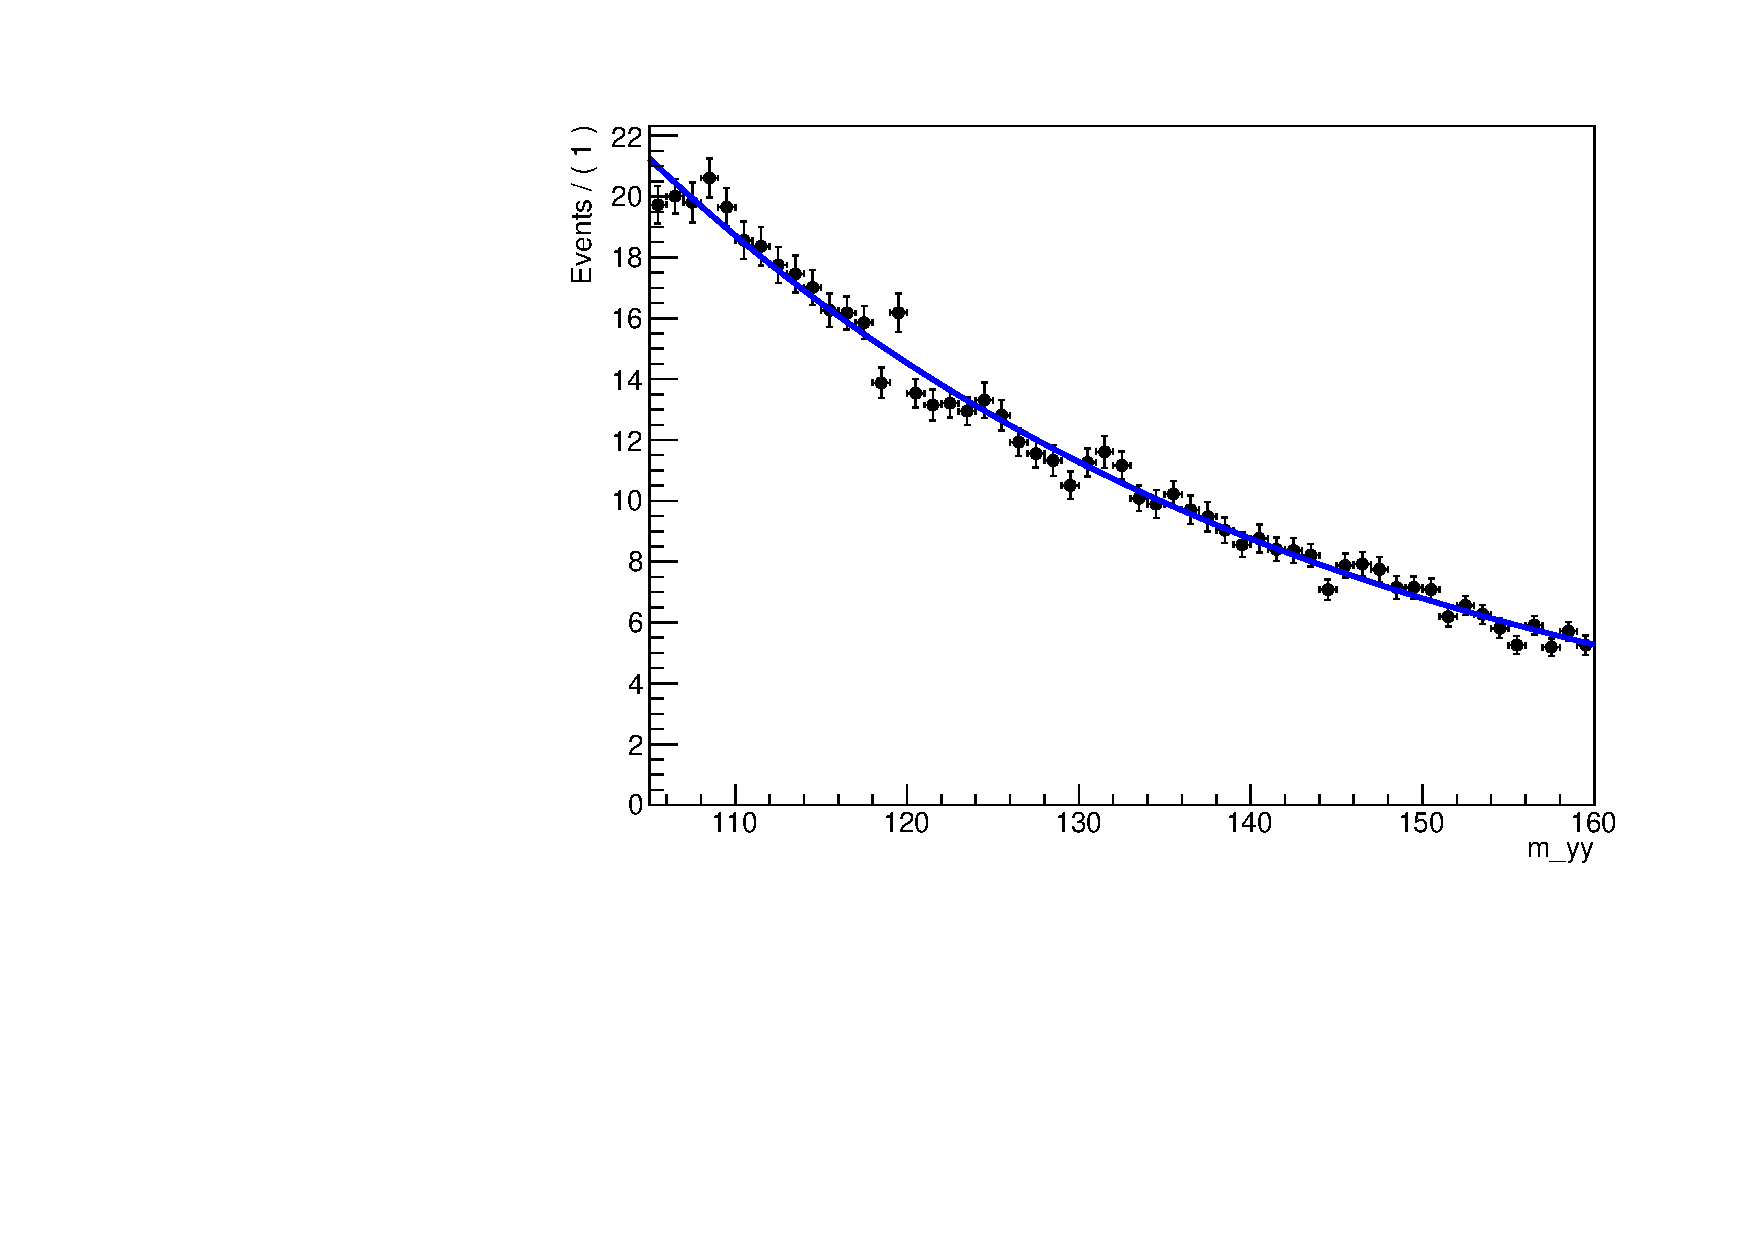
\includegraphics[width=0.48\textwidth]{chapters/chapter5_yybb/images/parameterization/fit_exp_1taglow}}
  \subfloat[High mass selection, 1 b-tag]{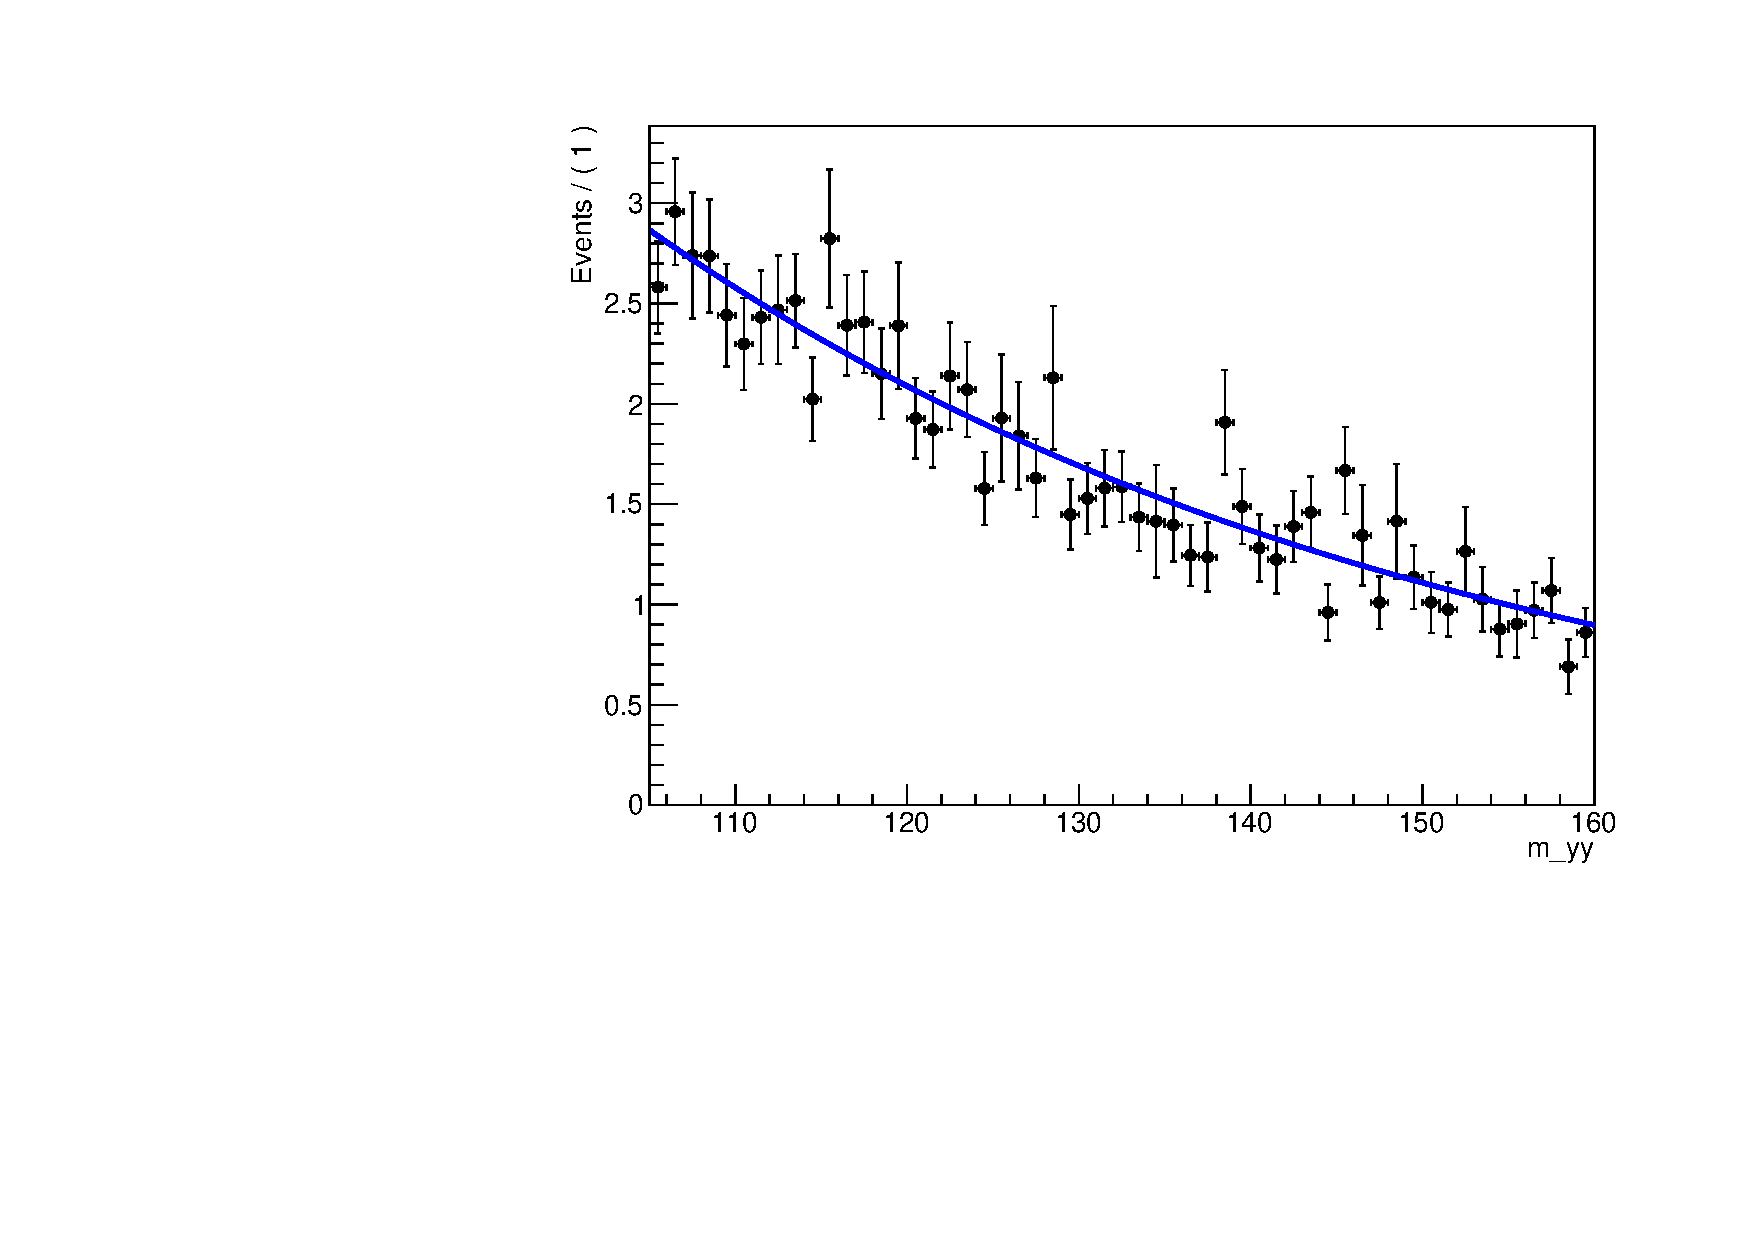
\includegraphics[width=0.48\textwidth]{chapters/chapter5_yybb/images/parameterization/fit_exp_1taghigh}}\\
  \subfloat[Low mass selection, 2 b-tag]{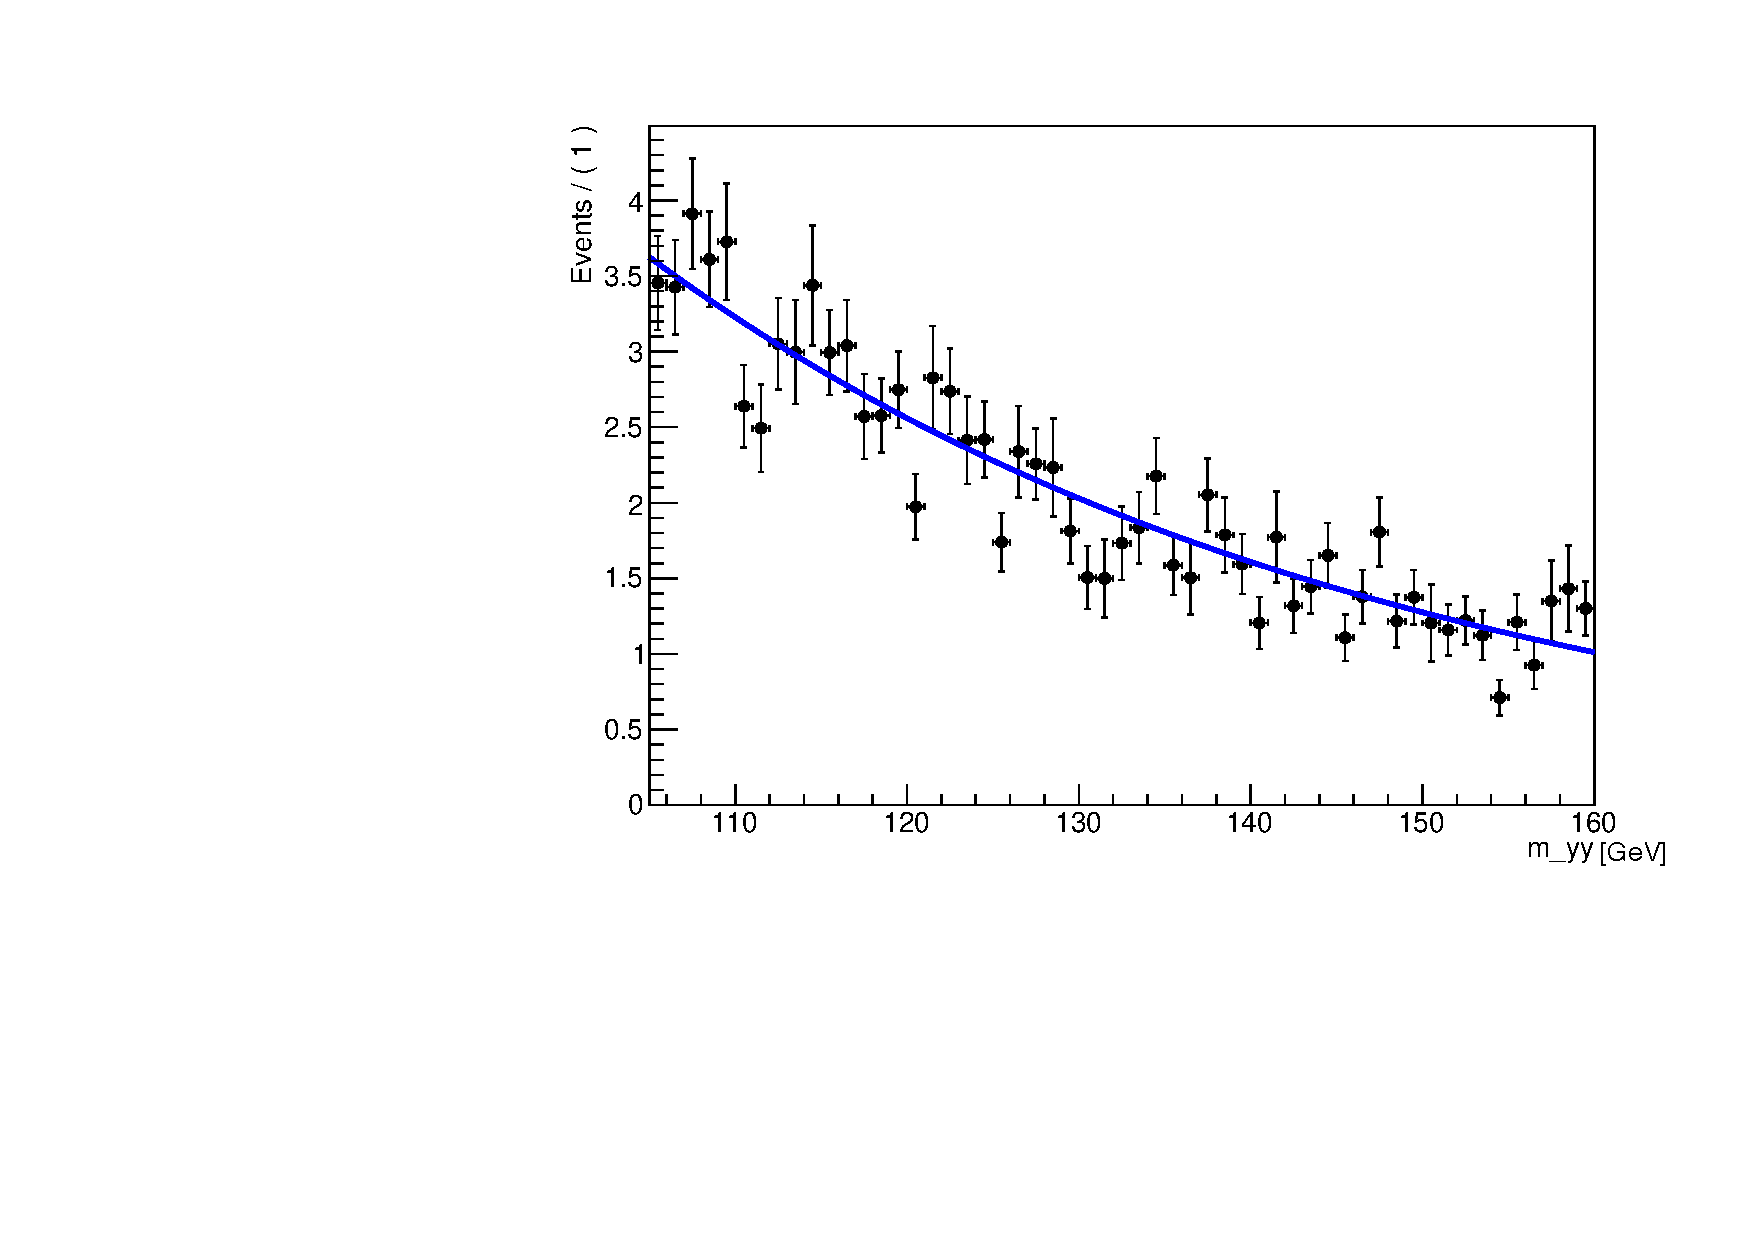
\includegraphics[width=0.48\textwidth]{chapters/chapter5_yybb/images/parameterization/fit_exp_2taglow}}
  \subfloat[High mass selection, 2 b-tag]{\includegraphics[width=0.48\textwidth]{chapters/chapter5_yybb/images/parameterization/fit_exp_2taghigh}}
  \caption[Background-only fit to the $\myy$ distribution using the first-order exponential function]{Background-only fit to the $\myy$ distribution using the low and high-mass selections, for the 1 and 2 b-tag categories using the first-order exponential function.}
  \label{fig:bkg-fit-myy}
\end{figure}


The single Higgs boson background is modeled through a double-sided Crystal Ball function, where parameters are taken from simulation. These fits are shown in Figure \ref{fig:SMh_DoubleCB}.

\begin{figure}[t!]
  \centering
  \includegraphics[width=0.48\textwidth]{{chapters/chapter5_yybb/images/parameterization/plot_singleRes_m125.SM_DSCB_c1}.eps}
  \includegraphics[width=0.48\textwidth]{{chapters/chapter5_yybb/images/parameterization/plot_singleRes_m125.SM_DSCB_c2}.eps}
  \caption[SM single Higgs \myy parameterization with a double-sided Crystal Ball function]{Parameterization of the \myy distribution from the SM single-Higgs simulated samples at a mass of 125 GeV in the 1-tag (left) and 2-tag (right) categories. Events were required to pass the high mass selection.
  \label{fig:SMh_DoubleCB}}
  \end{figure}
  

\subsection{Modeling in the Resonant Analysis}
\subsubsection{Signal Modeling}

For the resonant analysis, several functional forms were considered, including \texttt{ExpGaussExp}\footnote{Also called a ``double-shouldered GaussExp.''}, Crystal Ball + Gaussian, Crystal Ball + Voigt, and a Double Sided Crystal Ball. The model with the fewest parameters that converged was selected. This model was the \texttt{ExpGaussExp}, a function using a gaussian core with exponential tails. The mass hypotheses were fit simultaneously, which this yielded more stable fits. Sample fits for two mass hypotheses, one high mass (750 GeV) and one low mass (325 GeV), are shown in Figure \ref{fig:resonant_myybb_EGE}.

\begin{figure}[htbp!]
  \centering
  
  \subfloat[325 GeV, 1 b-tag, low mass selection]{\includegraphics[width=0.48\textwidth]{chapters/chapter5_yybb/images/parameterization/signal_model_EGE_lowMass_1tag_mX_325.pdf}}
  \subfloat[325 GeV, 2 b-tag, low mass selection]{\includegraphics[width=0.48\textwidth]{chapters/chapter5_yybb/images/parameterization/signal_model_EGE_lowMass_2tag_mX_325.pdf}}\\
  \subfloat[750 GeV, 1 b-tag, high mass selection]{\includegraphics[width=0.48\textwidth]{chapters/chapter5_yybb/images/parameterization/signal_model_EGE_highMass_1tag_mX_750.pdf}}
  \subfloat[750 GeV, 2 b-tag, high mass selection]{\includegraphics[width=0.48\textwidth]{chapters/chapter5_yybb/images/parameterization/signal_model_EGE_highMass_2tag_mX_750.pdf}}
  

  \caption[\myybb\ parameterization for resonant samples using an \texttt{ExpGaussExp} function]{Parameterization with an \texttt{ExpGaussExp} of the $\myybb$ distribution from one low mass (325 GeV) and one high mass (750 GeV) resonant di-Higgs sample. The mass hypotheses, selection used, and b-tag category are indicated.
  \label{fig:resonant_myybb_EGE}}
\end{figure}

  


\subsubsection{Background Modeling} \label{sssec:res-bkg-model}

Similar to the non-resonant analysis, a spurious signal test (described in Section \ref{sssec:nonres-bkg-model}) is performed to select the background fit function. The fit function is performed in both the 1 and 2-tag categories, where the same generalized fit function is required to be used to correlate uncertainties, however the parameter values can differ between categories. Different fit functions are selected for the low and high mass categories, where the low mass fit must contain a characteristic peak, and the high mass fit must be monotonically decreasing. For the low mass region (using the loose selection), the following functions were considered:

\begin{itemize}
  \item Novosibirsk: $P(x) = exp(-0.5^{ln(q_y)^2 / \Lambda^2 + \Lambda^2})$ with $q_{y} = 1 + \Lambda(x-x_0)/\sigma \times \frac{\sinh(\Lambda \sqrt{\ln(4)})}{\Lambda \sqrt{\ln(4)}}$.
  \item Modified Gamma: a Gamma distribution where the shape and scale parameters are replaced by linear functions of the mass hypothesis. This adds 2 additional degrees of freedom (5 total).
  \item Modified Landau: a Landau distribution where the shape parameter is replaced by a linear function of the mass hypothesis. This adds 1 additional degree of freedom (3 total).
\end{itemize}


For the high mass region (using the tight selection), the following functions were considered:
\begin{itemize}
  \item Exponential ($x$): $Exp[x](\myybb;p_0) = exp(p_0 \cdot \myybb)$
  \item Exponential ($x^2$): $Exp[x^2](\myybb;p_0) = exp(p_0 \cdot \myybb^{2})$
  \item Inverse polynomial ($x^{-2}$): $Inv\ Poly [x^{-2}](\myybb;p_0) = 1 +p_0/(\myybb^{2})$
  \item Inverse polynomial ($x^{-3}$): $Inv\ Poly [x^{-3}](\myybb;p_0) = 1 +p_0/(\myybb^{3})$
  \item Power Law: $Power\ Law(\myybb;p_0) = \myybb^{p_0}$
\end{itemize}

The number of spurious signal events were obtained by performing S+B fits in the \myybb spectrum separately in the 1 and 2-tag categories. For the low mass region, the fits were performed from 245 GeV to 485 GeV, for the high mass region the fits were performed from 335 GeV to 1140 GeV, which correspond to 95\% signal coverage of the resonant masses considered. The results of the 1-tag spurious signal test are shown in Table \ref{tab:spurious-signal-1}, and the 2-tag results are shown in Table \ref{tab:spurious-signal-2}, with the systematic uncertainty on the signal amplitude in terms of spurious signal $N_{spur}$ and its ratio to the statistical uncertainty on the fitted number of signal events $Z_{spur}$ is its ratio the fitted number of signal events.

The Novosibirsk function is selected for the low mass region and the exponential function is selected for the high mass region. For the 2 \btag category, more complicated functions have slightly smaller $N_{spur}$, but failed to fit high-mass distributions well in pseudodata trials. Background-only fits to using these functions are shown for the 1 and 2 b-tag categories in Figure \ref{fig:bkg-fit-myyjj}.

\begin{table}[!h]
  \centering
  \caption[Spurious signal test results for the 1 b-tag category]{Spurious signal test results for the 1 b-tag category. $N_{spur}$ is the spurious signal amplitude, $Z_{spur}$ is its ratio the fitted number of signal events. $\chi^2$/ndof values is obtained from a background-only fit. Parameters gives the number of floating parameters in the given function.}
  \label{tab:spurious-signal-1}
  \begin{tabular}{|c|c|c|c|c|}
    \hline
    \multicolumn{5}{|c|}{Low Mass}\\
    \hline
    Model     &   Maximum $Z_{spur}$ [\%]      &      Maximum $N_{spur}$      &   Parameters     &    $\chi^2$/ndof \\
    \hline
    Novosibirsk        & 33.64    &   2.06  & 3  & 36.7/22 \\
    Modified Gamma     & 53.67    &   3.42  & 5  & 45.2/20 \\
    Modified Landau    & 96.93    &   7.54  & 3  & 128.3/22 \\
    \hline
    \multicolumn{5}{|c|}{High Mass}\\
    \hline
    Model     &   Maximum $Z_{spur}$ [\%]      &      Maximum $N_{spur}$      &   Parameters     &    $\chi^2$/ndof \\
    \hline
    Exp ($x$)             &  63.66    &  0.89  & 1  & 32.5/26 \\
    Exp ($x^2$)           &  73.64    &  0.97  & 1  & 53/9/26 \\
    Inv. Poly ($x^-2$)    &  355.52   &  1.51  & 1  & 354.7/26 \\
    Inv. Poly ($x^-3$)    &  146.35   &  1.03  & 1  & 68.8/26 \\
    Power Law             &  78.00    &  0.96  & 1  & 45.0/26 \\
    \hline    
  \end{tabular}
\end{table}

\begin{table}[!h]
  \centering
  \caption[Spurious signal test results for the 2 b-tag category]{Spurious signal test results for the 2 b-tag category. $N_{spur}$ is the spurious signal amplitude, $Z_{spur}$ is its ratio the fitted number of signal events. $\chi^2$/ndof values is obtained from a background-only fit. Parameters gives the number of floating parameters in the given function.}
  \label{tab:spurious-signal-2}
  \begin{tabular}{|c|c|c|c|c|}
    \hline
    \multicolumn{5}{|c|}{Low Mass}\\
    \hline
    Model     &   Maximum $Z_{spur}$ [\%]      &      Maximum $N_{spur}$      &   Parameters     &    $\chi^2$/ndof \\
    \hline
    Novosibirsk        & 56.97    &  0.58   & 3  & 33.9/22 \\
    Modified Gamma     & 82.05    &  0.77   & 5  & 36.3/20 \\
    Modified Landau    & 65.62    &  1.09   & 3  & 45.8/22 \\
    \hline
    \multicolumn{5}{|c|}{High Mass}\\
    \hline
    Model     &   Maximum $Z_{spur}$ [\%]      &      Maximum $N_{spur}$      &   Parameters     &    $\chi^2$/ndof \\
    \hline
    Exp ($x$)             &  98.94   & 0.21   & 1  & 36.4/26 \\
    Exp ($x^2$)           &  123.18   & 0.27   & 1  & 59.0/26 \\
    Inv. Poly ($x^-2$)    &  88.33   & 0.25   & 1  & 42.9/26 \\
    Inv. Poly ($x^-3$)    &  116.84   & 0.13   & 1  & 22.2/26 \\
    Power Law             &  72.46   & 0.17   & 1  & 25.9/26 \\
    \hline    
  \end{tabular}
\end{table}


\begin{figure}[htbp!]
  \centering
  \subfloat[1 b-tag, low mass]{\includegraphics[width=0.48\textwidth]{chapters/chapter5_yybb/images/parameterization/m_yyjj_lowMass_1tag_bkgOnly}}
  \subfloat[1 b-tag, high mass]{\includegraphics[width=0.48\textwidth]{chapters/chapter5_yybb/images/parameterization/m_yyjj_highMass_1tag_bkgOnly}}\\
  \subfloat[2 b-tag, low mass]{\includegraphics[width=0.48\textwidth]{chapters/chapter5_yybb/images/parameterization/m_yyjj_lowMass_2tag_bkgOnly}}
  \subfloat[2 b-tag, high mass]{\includegraphics[width=0.48\textwidth]{chapters/chapter5_yybb/images/parameterization/m_yyjj_highMass_2tag_bkgOnly}}
  \caption[Background-only fit to the \myybb distribution]{Background-only fit to the \myybb distribution. The b-tag category and selection used is indicated.}
  \label{fig:bkg-fit-myyjj}
\end{figure}


\section{Systematic Uncertainties}

As a result of the small \hh cross-section, the sensitivity of this analysis is dominated by statistical uncertainties\footnote{The statistical uncertainties are taken as Poisson uncertainties ($1/\sqrt{N}$).}. The following sections will discuss systematic uncertainties, both theoretical (Section \ref{ssec:theory-unc}) and experimental (Section \ref{ssec:exp-unc}).

\subsection{Theoretical Uncertainties} \label{ssec:theory-unc}

This section describes theoretical uncertainties on the mono-Higgs and di-Higgs samples. In each of these, alternate models of parton showering and hadronization were considered and differences were found to be negligible.

\noindent\textbf{Mono-Higgs:} Theory uncertainties for the mono-Higgs boson production cross-section are estimated through varying renormalization and factorization scales. These scale uncertainties reach $^{+20\%}_{-24\%}$. Uncertainties due to the \gls{PDF} and running of the \gls{QCD} coupling constant ($\alpha_{S}$) are also considered, reaching $\pm3.6\%$. Production associated with heavy-flavor jets is considered as follows:

\begin{itemize}
  \item $ggH$ and $ZH$: A 100\% uncertainty is assigned, motivated by previous studies of heavy-flavor production with top quark pairs \cite{heavy-flavor-top} and $W$ boson production in association with b-jets \cite{heavy-flavor-W}.
  \item $ZH$ and \tth: No heavy-flavor uncertainty assigned. The dominant contribution is accounted for in the \gls{LO} process.
\end{itemize}

A $H\rightarrow \yy$ \gls{BR} uncertainty of $^{+2.9\%}_{-2.8\%}$ and a $H\rightarrow \bb$ \gls{BR} uncertainty of $\pm1.7\%$ \cite{hh-crosssections} are taken into account as well.

\noindent\textbf{\gls{SM} Di-Higgs:} The \gls{SM} \hh signal samples are impacted by the same theory uncertainties as the mono-Higgs, as described above. For the \gls{NNLO} cross-section, the scale effects are 4-8\%, and the $\text{PDF}+\alpha_{S}$ uncertainty is 2-3\%. An additional 5\% uncertainty is added from the infinite top-quark mass approximation \cite{nnlo-topquark}.

\noindent\textbf{Resonant Di-Higgs:} For the resonant analysis, scale and \gls{PDF} uncertainties are neglected. The \gls{SM} non-resonant \hh production is a background with uncertainty $^{+7\%}_{-8\%}$, and interference between the resonant \hh signal and nonresonant \hh production is neglected.

\subsection{Experimental Uncertainties} \label{ssec:exp-unc}

\noindent\textbf{Luminosity:} Beam-separation scans in 2015 and 2016 are used to derive the systematic uncertainty in the integrated luminosity of 2.1\%. This methodology is outlined in Reference \cite{lumi-unc}.

\noindent\textbf{Trigger:} Bootstrap methods presented in Reference \cite{trigger-unc} are used to determine the efficiency of the diphoton trigger. This trigger is 99.4\% efficient with a systematic of 0.4\%.

\noindent\textbf{Simulation:} Calibration uncertainties apply to photons and jets used in the analysis, for all samples except the \yy-continuum, which is estimated from data. The uncertainties are propagated through the analysis chain, and relevant observables are constructed. Then changes in peak location and width ($m_{\text{peak}}$ and $\sigma_{\text{peak}}$, respectively), as well as signal yield in \myy (non-resonant) or \myybb (resonant) are extracted. In the resonant analysis, uncertainties are evaluated at each mass hypothesis are evaluated, and the maximum value is taken.

\noindent\textbf{Yield:} Photon identification and isolation affect the diphoton selection efficiency. Peak uncertainties are primarily due to photon energy scale, and are about 0.2-0.6\% for both mono and di-Higgs samples. Width uncertainties are primarily due to photon energy resolution, and are 5-14\%. Uncertainties in \gls{JES} and \gls{JER} affect the \mbb acceptance \cite{jes-uncertainty}.  Uncertainties in flavor tagging can miscategorization of events in the tagging categories. A summary of the most dominant systematic uncertainties can be found in Table \ref{tab:systematic_uncertainties}

\noindent\textbf{Signal Model:} The spurious signal, described in Section \ref{sssec:nonres-bkg-model}, is used as an uncertainty on the number of signal events. The values for each analysis category can be found in Table \ref{tab:unc-sig-events}.

\begin{table}[htbp]
  \centering
  \caption[Uncertainty on total number of signal events in each analysis category]{Uncertainty on total number of signal events in each analysis category, as derived from the spurious signal test}
  \label{tab:unc-sig-events}
  \begin{tabular}{c|c|c}
    Analysis & Category & Uncertainty on Number of Events \\
    \hline 
    Non-resonant &\makecell{1-tag\\2-tag} & \makecell{0.25\\0.63}\\
    \hline
    Resonant & \makecell{Loose\\Tight} & \makecell{0.21\\0.89}\\
  \end{tabular}
\end{table}

\noindent\textbf{Cross Section:} In the resonant analysis, an $m_X$ correction is applied to the signal cross-section. This, along with its associated uncertainty is applied at low mass to adjust for degeneracy biases. %% TODO: make sure this is clear elsewhere, reference?


%%%%%% SYSTEMATICS TABLE
\begin{table}[!htb]
  \begin{center}
    %TODO - reword this
  \caption[Summary of dominant systematic uncertainties affecting expected yields in the resonant and non-resonant analyses]{Summary of dominant systematic uncertainties affecting expected yields in the resonant and non-resonant analyses.
      For the non-resonant analysis, uncertainties in the Higgs boson pair signal and SM single-Higgs-boson backgrounds are presented.
      For the resonant analysis, uncertainties on the Higgs boson pair signal for the loose and tight selections are presented.
      Sources marked `-' and other sources not listed in the table are negligible by comparison.
      No systematic uncertainties related to the continuum background are considered, since this is derived through a fit to the observed data.}
  \label{tab:systematic_uncertainties}

      \resizebox{\textwidth}{!}
      {\normalsize
          \begin{tabular}{l l r@{} @{}D{.}{.}{1.1} r@{} @{}r@{} @{}D{.}{.}{1.1}@{} @{}l r@{} @{}D{.}{.}{1.1} r@{} @{}r@{} @{}D{.}{.}{2.1}@{} @{}l r@{} @{}D{.}{.}{1.1} r@{} @{}r@{} @{}D{.}{.}{1.1}@{} @{}l r@{} D{.}{.}{1.1} r@{} @{}r@{} @{}D{.}{.}{1.1}@{} @{}l}
                  \toprule
              \multicolumn{2}{c}{\multirow{2}{*}{Source of systematic uncertainty}}                                 & \multicolumn{24}{c}{\% effect relative to nominal in the 2-tag (1-tag) category}                                                                   \\
                                                       &                                                            & \multicolumn{12}{c}{Non-resonant analysis}                             & \multicolumn{12}{c}{Resonant analysis: BSM \hh}                           \\
              \midrule
                                                       &                                                            & \multicolumn{6}{c}{SM \hh signal} & \multicolumn{6}{c}{Single-$H$ bkg} & \multicolumn{6}{c}{Loose selection} & \multicolumn{6}{c}{Tight selection} \\
              \midrule
              \multicolumn{2}{l}{Luminosity}                                                                        & $\pm$ & 2.1 & ( & $\pm$ & 2.1 & ) & $\pm$ & 2.1 & ( & $\pm$ & 2.1  & ) & $\pm$ & 2.1 & ( & $\pm$ & 2.1 & )   & $\pm$ & 2.1 & ( & $\pm$ & 2.1 & )   \\
              \multicolumn{2}{l}{Trigger}                                                                           & $\pm$ & 0.4 & ( & $\pm$ & 0.4 & ) & $\pm$ & 0.4 & ( & $\pm$ & 0.4  & ) & $\pm$ & 0.4 & ( & $\pm$ & 0.4 & )   & $\pm$ & 0.4 & ( & $\pm$ & 0.4 & )   \\
              \multicolumn{2}{l}{Pile-up modelling}                                                                 & $\pm$ & 3.2 & ( & $\pm$ & 1.3 & ) & $\pm$ & 2.0 & ( & $\pm$ & 0.8  & ) & $\pm$ & 4.0 & ( & $\pm$ & 4.2 & )   & $\pm$ & 4.0 & ( & $\pm$ & 3.8 & )   \\
              \midrule
              \multirow{4}{*}{Photon}                  & identification                                             & $\pm$ & 2.5 & ( & $\pm$ & 2.4 & ) & $\pm$ & 1.7 & ( & $\pm$ & 1.8  & ) & $\pm$ & 2.6 & ( & $\pm$ & 2.6 & )   & $\pm$ & 2.5 & ( & $\pm$ & 2.5 & )   \\
                                                       & isolation                                                  & $\pm$ & 0.8 & ( & $\pm$ & 0.8 & ) & $\pm$ & 0.8 & ( & $\pm$ & 0.8  & ) & $\pm$ & 0.8 & ( & $\pm$ & 0.8 & )   & $\pm$ & 0.9 & ( & $\pm$ & 0.9 & )   \\
                                                       & energy resolution                                          & \multicolumn{6}{c}{-}             & \multicolumn{6}{c}{-}              & $\pm$ & 1.0 & ( & $\pm$ & 1.3 & )   & $\pm$ & 1.8 & ( & $\pm$ & 1.2 & )   \\
                                                       & energy scale                                               & \multicolumn{6}{c}{-}             & \multicolumn{6}{c}{-}              & $\pm$ & 0.9 & ( & $\pm$ & 3.0 & )   & $\pm$ & 0.9 & ( & $\pm$ & 2.4 & )   \\
              \midrule
              \multirow{2}{*}{Jet}                     & energy resolution                                          & $\pm$ & 1.5 & ( & $\pm$ & 2.2 & ) & $\pm$ & 2.9 & ( & $\pm$ & 6.4  & ) & $\pm$ & 7.5 & ( & $\pm$ & 8.5 & )   & $\pm$ & 6.4 & ( & $\pm$ & 6.4 & )   \\
                                                       & energy scale                                               & $\pm$ & 2.9 & ( & $\pm$ & 2.7 & ) & $\pm$ & 7.8 & ( & $\pm$ & 5.6  & ) & $\pm$ & 3.0 & ( & $\pm$ & 3.3 & )   & $\pm$ & 2.3 & ( & $\pm$ & 3.4 & )   \\
              \midrule
              \multirow{3}{*}{Flavor tagging}         & $b$-jets                                                   & $\pm$ & 2.4 & ( & $\pm$ & 2.5 & ) & $\pm$ & 2.3 & ( & $\pm$ & 1.4  & ) & $\pm$ & 3.4 & ( & $\pm$ & 2.6 & )   & $\pm$ & 2.5 & ( & $\pm$ & 2.6 & )   \\
                                                       & $c$-jets                                                   & $\pm$ & 0.1 & ( & $\pm$ & 1.0 & ) & $\pm$ & 1.8 & ( & $\pm$ & 11.6 & ) & \multicolumn{6}{c}{-}               & \multicolumn{6}{c}{-}               \\
                                                       & light-jets                                                 & $<$   & 0.1 & ( & $\pm$ & 5.0 & ) & $\pm$ & 1.6 & ( & $\pm$ & 2.2  & ) & \multicolumn{6}{c}{-}               & \multicolumn{6}{c}{-}               \\
              \midrule
              \multirow{4}{*}{Theory}                  & PDF{+}$\alpha_{S}$                                            & $\pm$ & 2.3 & ( & $\pm$ & 2.3 & ) & $\pm$ & 3.1 & ( & $\pm$ & 3.3  & ) & \multicolumn{6}{c}{n/a}             & \multicolumn{6}{c}{n/a}             \\
                                                       & \multirow{2}{*}{Scale}                                     & $+$   & 4.3 & ( & $+$   & 4.3 & ) & $+$   & 4.9 & ( & $+$   & 5.3  & ) & \multicolumn{6}{c}{n/a}             & \multicolumn{6}{c}{n/a}             \\
                                                       &                                                            & $-$   & 6.0 & ( & $-$   & 6.0 & ) & $+$   & 7.0 & ( & $+$   & 8.0  & ) & \multicolumn{6}{c}{n/a}             & \multicolumn{6}{c}{n/a}             \\
                                                       & EFT                                                        & $\pm$ & 5.0 & ( & $\pm$ & 5.0 & ) & \multicolumn{6}{c}{n/a}            & \multicolumn{6}{c}{n/a}             & \multicolumn{6}{c}{n/a}             \\
              \bottomrule
          \end{tabular}
      }
  \end{center}
\end{table}
%%%%%% SYSTEMATICS TABLE



\section{Results}

\subsection{Limits on Non-Resonant Production}

The tight selection is used in the non-resonant analysis to set a 95\% \gls{CL} upper limit on non-resonant \gls{ggF} Higgs boson pair production. The observed and expected limits are shown Table \ref{tab:nonresonant_results_SM} in both absolute value and as a multiple of the \gls{SM} production cross-section. The observed $\pm 1\sigma$ values are shown as well. This upper limit is shown in Figure \ref{fig:limits-nonresonant}, and the data and background-only fit on the \myy spectrum is shown in Figure \ref{fig:results-myy}.

\begin{table}[htbp]
  \centering 
  \caption{Non-resonant limits in terms of the Standard Model HH cross section}
  \label{tab:nonresonant_results_SM} 

  \begin{tabular}{ccccc}
  \hline
  & Observed & Expected & $-1\sigma$  & $+1\sigma$ \\
  \hline
  $\sigma_{gg\rightarrow HH}$ [pb] & 0.73 & 0.93 & 0.66 & 1.3\\
  Multiple of $\sigma_{SM}$ & 22 & 28 & 20 & 40 \\
  \hline
  \end{tabular}
\end{table}

\begin{figure}[htbp]
	\subfloat[]{\includegraphics[width=0.48\textwidth]{chapters/chapter5_yybb/images/results/m_yy_lowMass_1tag_bkg_fit_to_data_withRatio}}
	\quad
	\subfloat[]{\includegraphics[width=0.48\textwidth]{chapters/chapter5_yybb/images/results/m_yy_lowMass_2tag_bkg_fit_to_data_withRatio}}
	\\
	\subfloat[]{\includegraphics[width=0.48\textwidth]{chapters/chapter5_yybb/images/results/m_yy_highMass_1tag_bkg_fit_to_data_withRatio}}
	\quad
	\subfloat[]{\includegraphics[width=0.48\textwidth]{chapters/chapter5_yybb/images/results/m_yy_highMass_2tag_bkg_fit_to_data_withRatio}}
	\caption{Data and background-only fits for each of the analysis categories in the non-resonant analysis. The background fit is composed of the smoothly-falling continuum \yy background as well as the single Higgs boson production background, peaking around $\unit{125}{\GeV}$.}
  \label{fig:results-myy}
\end{figure}


\begin{figure}[htbp]
  \centering
\includegraphics[width=0.9\textwidth]{chapters/chapter5_yybb/images/limits/nonresonant.pdf}
  \caption[The expected and observed limits on the non-resonant HH production cross section]
  {The expected and observed 95\% \gls{CL} limits on the non-resonant HH production cross section, $\sigma_{gg\rightarrow HH}$. These limits are set using the tight analysis selection. The 95\% confidence level is indicated by the red horizontal line.}
  \label{fig:limits-nonresonant}
\end{figure}

\subsection{Limits on Resonant Production}

The 95\% \gls{CL} limits on resonant di-Higgs production are shown in Figure \ref{fig:limits-resonant}. This limit uses the loose selection at $m_{X} \leq \unit{500}{\GeV}$ and the tight selection at $m_{X} \geq \unit{500}{\GeV}$. No significance excesses are found. Expected exclusion limits range from 1.14 pb to 0.12 pb, observed limits range from 0.90 pb to 0.15 pb.

\begin{figure}[htbp]
  \centering
\includegraphics[width=0.9\textwidth]{chapters/chapter5_yybb/images/limits/resonant.pdf}
\caption[The expected and observed limits on the resonant \HH production cross section as a function of $m_{X}$.]
{The expected and observed 95\% \gls{CL} limits on the resonant \HH production cross-section, $\sigma_{X} \times \mathcal{B}(X\rightarrow HH)$, as a function of $m_{X}$. The loose selection is used in the low mass regime, $m_{X} \leq \unit{500}{\GeV}$, while the tight selection is used in the high mass regime, $m_{X} \geq \unit{500}{\GeV}$. The transition point between these selections is indicated by the dashed line.} 
\label{fig:limits-resonant}
\end{figure}

\subsection{Limits on the Trilinear Higgs Coupling}

Limits are set on \klambda using the asymptotic formula. The exclusion as a function of \klambda is shown in Figure \ref{fig:limits-klambda}, corresponding to $-8.2 < \klambda < 13.3$.

\begin{figure}[htbp]
  \centering
\includegraphics[width=0.9\textwidth]{chapters/chapter5_yybb/images/limits/lambda.pdf}
\caption[The expected and observed limits on the non-resonant \HH production cross section as a function of \klambda]
{The expected and observed 95\% \gls{CL} limits on the non-resonant \HH production cross section as a function of \klambda. The red line indicated the predicted $HH$ cross-section for varied \klambda, assuming all other couplings are equivalent to \gls{SM} prediction, the band includes theoretical uncertainty.} 
\label{fig:limits-klambda}
\end{figure}